% IAU_Sample.tex -- sample pages for Proceedings IAU Symposium document class
% (based on v1.0 cca2esam.tex)
% v1.04 released 17 May 2004 by TechBooks
%% small changes and additions made by KAvdH/IAU 4 June 2004
% Copyright (2004) International Astronomical Union
% Minor updates made for WriteLatex.com by Martyn Bristow
% ...Downloaded from http://www.iau.org/static/scientific_meetings/authors/ June 2014
\NeedsTeXFormat{LaTeX2e}

\documentclass{iau}
\usepackage{graphicx}
\usepackage{natbib}
\usepackage{siunitx}
\usepackage[utf8]{inputenc} % usually not needed (loaded by default)
\usepackage[T1]{fontenc}
\usepackage[english,spanish,french]{babel}
\newcommand{\magarc}{mag arcsec\ensuremath{^{\mathrm{-2}}}}
\newcommand{\RST}{\emph{Roman} Space Telescope}
\newcommand{\Euclid}{\emph{Euclid}}
\newcommand{\Hubble}{\emph{Hubble}}
\newcommand{\Gaia}{\emph{Gaia}}
\usepackage{url}

\title[JD 11.~~Chasing ghosts with Roman Space Telescope] %% give here short title %%
{Chasing ghosts with Roman Space Telescope}



\author[Alejandro S. Borlaff et al.]   %% give here short author list %%
{Alejandro S. Borlaff$^1$ \and Pamela M. Marcum$^1$ \and Scott Rohrbach$^2$ \and Pablo M. Sanchez-Alarcón$^1$ \and Seppo Laine $^3$}

\affiliation{$^1$NASA Ames Research Center, Moffett Field, CA 94035, USA \\ email: {\tt a.s.borlaff@nasa.gov} \\[\affilskip]
$^2$NASA Goddard Space Flight Center, 8800 Greenbelt Rd., Greenbelt, MD 20771\\ [\affilskip]
$^3$IPAC, Mail Code 314-6, Caltech, 1200 E. California Blvd., Pasadena, CA 91125, USA}

\pubyear{2008}
\volume{xxx}  %% insert here IAU Symposium No.
\pagerange{119--126}
% \date{?? and in revised form ??}
\setcounter{page}{1}
\jname{Title of your IAU Symposium}
\editors{A.C. Editor, B.D. Editor \& C.E. Editor, eds.}
\begin{document}
\include{variables}

\maketitle

\begin{abstract}
Diffuse emission in the outskirts of galaxies such as stellar tidal streams and intracluster light (ICL) provides crucial evidence for structure evolution and cosmology. However, these extended, low surface brightness (LSB) features are thousands of times dimmer than the sky background ($\mu\gtrsim 29$--$30$ AB \magarc, $0.5$--$2.3\,\mu$m). Unveiling this informative, yet hidden, emission with the \emph{Nancy Grace Roman} Space Telescope thus requires an exquisite control of large scale background gradients in the images.

In this contribution we describe \texttt{ROSALIA} (\emph{Roman} Sky Analyst for Low surface brightness Imaging \& Astronomy), a NASA pipeline to model the sky background level on astronomical images obtained with \emph{Nancy Grace Roman} Space Telescope focusing on the characterization of stray-light. \texttt{ROSALIA} uses ray-tracing models to perform a photometric analysis of secondary light paths that can reach of the WFI focal plane from out-of-field natural sources (i.e., stars, planets). We describe the predicted stray-light blocking efficiency of \emph{Roman}/WFI under several illumination conditions, and the calibration targets to be observed during the \emph{Roman}/WFI Commissioning. The products from this pipeline will enable \emph{Roman}/WFI to predict stray-light background levels generated by real sources in-orbit before observing and a more accurate removal of stray-light background in imaging observations, a critical step in low surface brightness astronomy and deep imaging. \texttt{ROSALIA} will be validated using end-to-end simulations of WFI mosaics, serving as an observation planning and calibration tool for the community, complementing current plans for WFI data processing by the mission.
\keywords{Space telescopes (1547), Space observatories (1543), Observational astronomy(1145), Calibration(2179) Interdisciplinary astronomy (804)}
%% add here a maximum of 10 keywords, to be taken form the file <Keywords.txt>
\end{abstract}

\firstsection % if your document starts with a section,
              % remove some space above using this command.
\section{Introduction}

One of the last frontiers in observational astronomy is the low surface brightness Universe ($\mu_{V}\gtrsim 27$ AB \magarc). This regime corresponds to the lowest stellar density regions in the Universe and have generally evaded detection by past, wide surveys \citep[i.e., SDSS,][]{york+2000aj120_1579}. Even from an L2 orbit, the darkest sky has a surface brightness of $\mu \sim22$ AB \magarc\ ($\lambda=0.5$--$2.3\,\mu$m). Only after removing of the Zodiacal light the dimmer spiral disks of galaxies become detectable ($\mu = 22$--$26$ AB \magarc). Tidal tails and other remnants of galactic collisions emit one order of magnitude less flux ($\mu= 26$--$28$ AB \magarc), and the dark matter dominated stellar halos are more than 1000 times dimmer than the sky background ($\mu= 29$--$31$ AB \magarc). Beyond the local Universe, cosmological dimming \citep{tolman1930nat16_511} significantly reduces the flux from such regions so that even relatively bright structures at high redshift are difficult to detect without deep imaging efforts, such as the \emph{Hubble Ultra Deep Field} \citep[][see Fig.\,\ref{fig:XDF}]{beckwith+2006aj132_1729,koekemoer+2013apj209_3,illingworth+2013apj209_6,borlaff+2019aap621_133}.\\


\begin{figure*}[t!]
\begin{center}
%\vspace{-0.3cm}
 % trim left bottom right top 
%\begin{overpic}[width=\textwidth, trim=0 0 0 0, clip]{FIGURES/abyss_vs_xdf_profile.png}
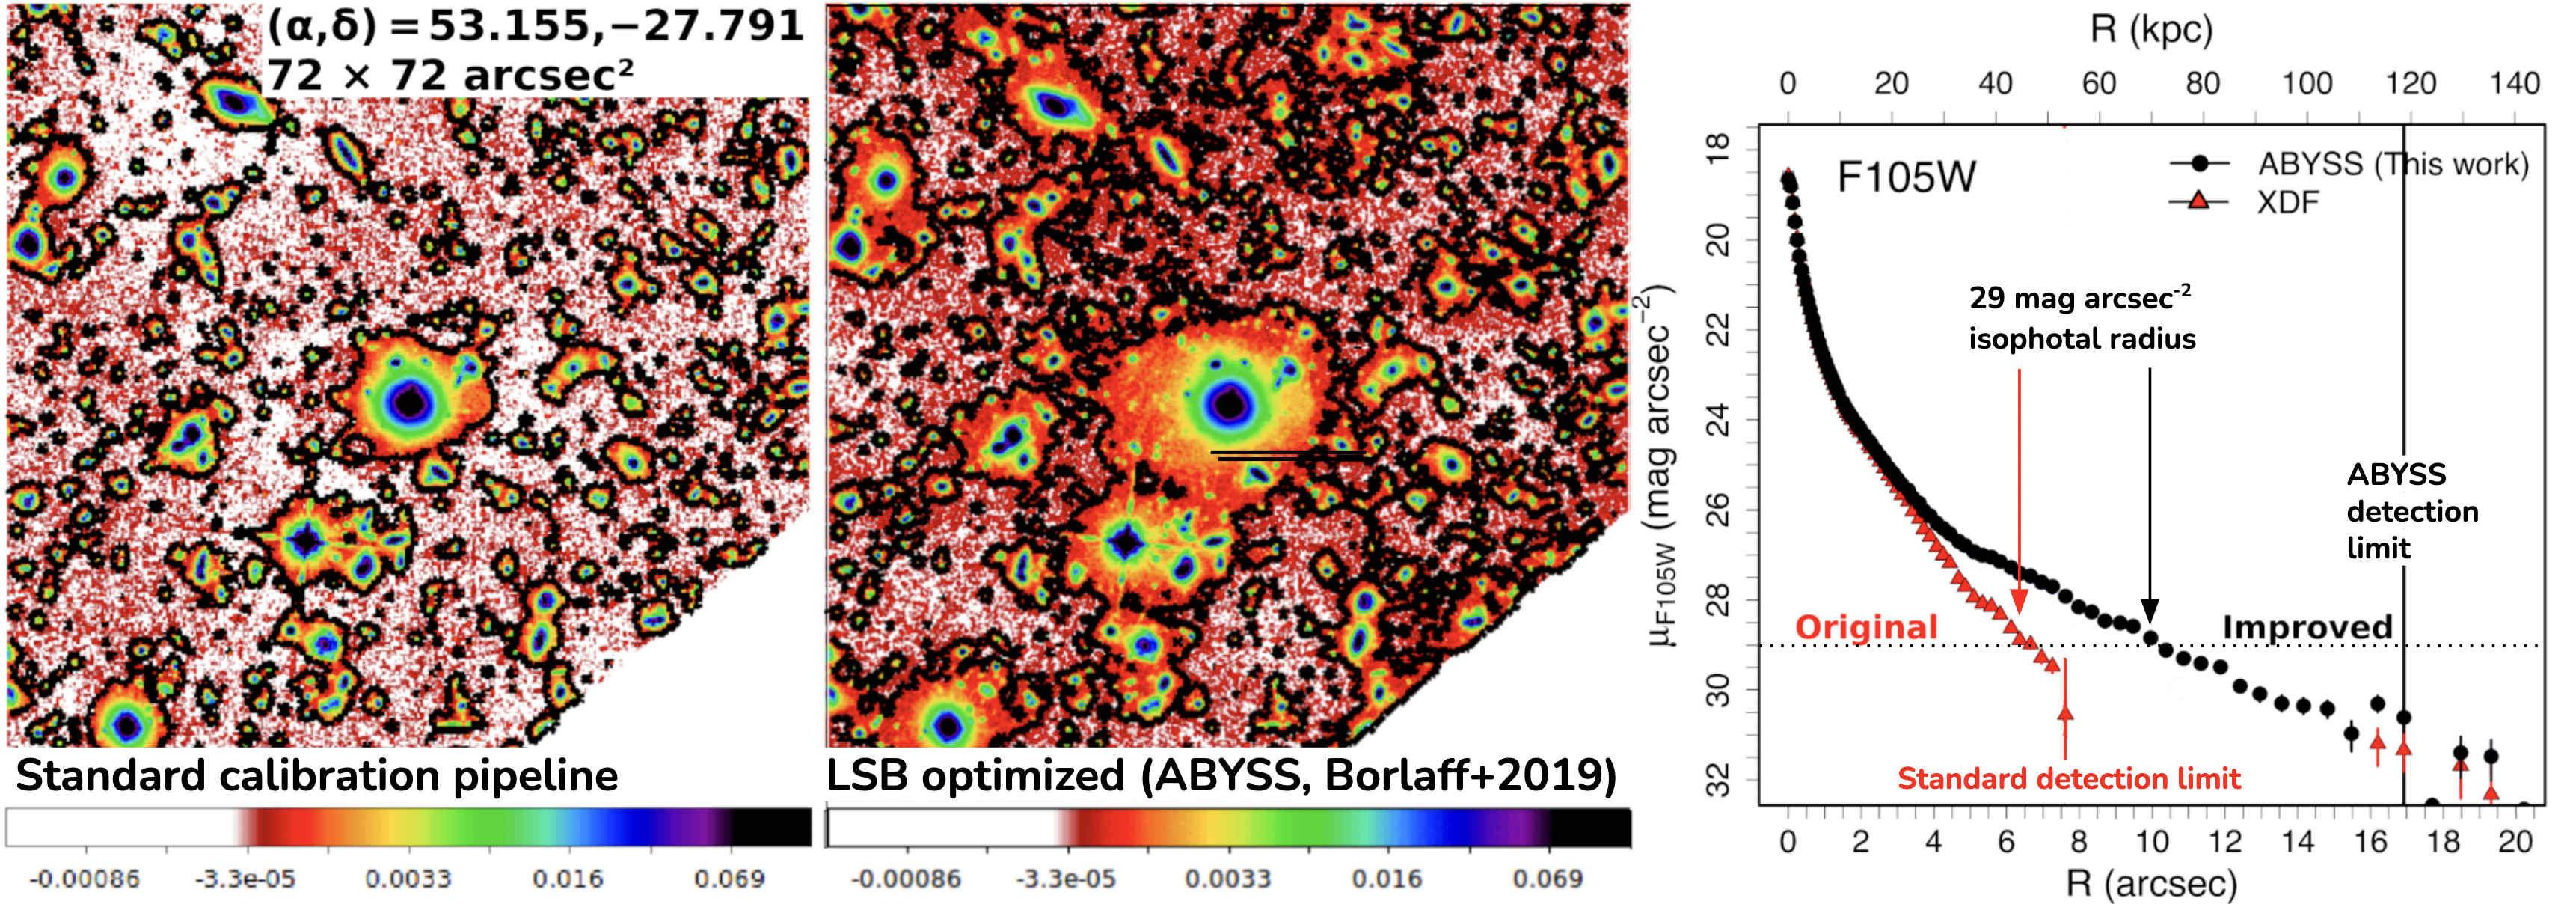
\includegraphics[trim={0 0 0 0}, clip, width=\textwidth]{abyss_vs_xdf_profile.png}
\caption{WFC3/IR F105W images centered on the HUDF-5 galaxy from the original XDF mosaics \citep[][left panel]{illingworth+2013apj209_6} and a low surface brightness improved pipeline \citep[ABYSS,][central panel]{borlaff+2019aap621_133}. The black contours represent the $\mu_{F105W} = 29$ \magarc\ isophote. Both images are at the same color scale, and were derived from the same raw datasets of \Hubble\ observations. \emph{Right panel:} Comparison of the surface brightness profiles of HUDF-5. The detection limit for the outskirts of the galaxy is $118$ kpc for the improved version vs. $53$ kpc for the original.}
\label{fig:XDF}
\end{center}
\end{figure*} 


Faint extended structures connect cosmological evolution to the assembly history of galaxies. The extended mass distribution of galactic disks was an early indication of the presence of dark matter \citep{freeman1970apj160_811} and deep optical/near infrared imaging has shown that diffuse stellar ICL directly traces the structure of dark matter halos \citep{montes+2019mnras482_2838}. Mass assembly pathways from dark matter models can be tested by counting the number of faint stellar streams that surround a galaxy \citep[a proxy of the number of past merging events, ][]{johnston+2008apj689_936}. Deep, wide field imaging surveys have also led to the discovery of a myriad of diffuse satellite galaxies, easing the tension of the ``missing satellite problem'' \citep{springel+2005nat435_629,martin+2019mnras485_796}, thereby providing a major test of the currently favored $\Lambda$ Cold Dark Matter cosmological paradigm \citep[e.g.,][]{moore+1999apj524_19,klypin+1999apj522_82, kim+2018prl121_211302}. Some objects are so dim and extended that, even today, they remain entirely invisible until serendipitous deep observations find them. The quasar-echo illuminated nebulae Hanny's Voorwerp \citep{jozsa+2009aap500_33}, giant low surface brightness galaxies like Malin 1 \citep{bothun+1987aj94_23}, ultra-diffuse galaxies \citep{vandokkum+2018nat555_629, montes+2020apj904_114}, or dim gas emission clouds \citep{drechsler+2023aas7_1, lumbrerascalle+2025aap704_224} suggest that our understanding of the Universe is entirely shaped by the sensitivity of current data.\\

For the study of these extended sources, the major limitation is not exposure time (this is, statistical noise) but separating real sources from background gradients (systematic effects). Sky background gradients can be generated by stray-light from sources (i.e., stars, planets), or by the telescope itself, like thermal emission, bias, or flat-field residuals. Due to the difficulty in modeling these effects, a sky background surface is typically fitted and subtracted from optical and infrared exposures \citep[][]{bertin+1996aap117_393}. Since most of the signal of dim extended sources is below the noise level on the individual exposures, this method tends to overestimate the sky under the astronomical target, creating an over-subtraction in the final mosaics. Sky background over-subtraction can remove all faint and extended signal \citep[i.e., stellar halos around galaxies;][]{akhlaghi+2015apj220_1}, severely restricting the discovery of sources hidden at the very low surface brightness limits of astronomical images.\\

Located in L2 orbit, with a FOV of $\ang{0.8;;}\times\ang{0.4;;}$, $\ang{;;0.1}$ of spatial resolution and a mirror diameter of 2.4 m, \RST\ will be an ideal observatory to study the low surface brightness Universe. We predict that \RST/WFI has the capability to achieve depths of $\mu_{\rm{lim}}=30.5$ \magarc\ in 30 minutes of exposure time in all of its filters from $0.5$ to $2\,\mu$m (except in F214, $\mu_{\rm{lim}}=28.8$ \magarc\ due to thermal self-emission, 3$\sigma$ detection in $\ang{;;10}\times\ang{;;10}$).  These detection limits are only possible with an optimal sky background correction to remove stray-light contamination in the individual exposures. The application of low surface brightness reduction techniques to \RST/WFI for large ($\sim1'$--$1^{\circ}$) sources goes beyond most of the mission's calibration plans, which focus on local sky background corrections to the images (several arcsec to perform photometry on high-$z$ targets). The development of a dedicated sky background calibration software specific to preserve the photometry of extended, ultra-low surface brightness sources with \RST\ is thus highly relevant for the scientific community.\\

\begin{figure*}[t!]
 \begin{center}
 % trim left bottom right top
\begin{minipage}{\textwidth}
  \centering
  \raisebox{-0.5\height}{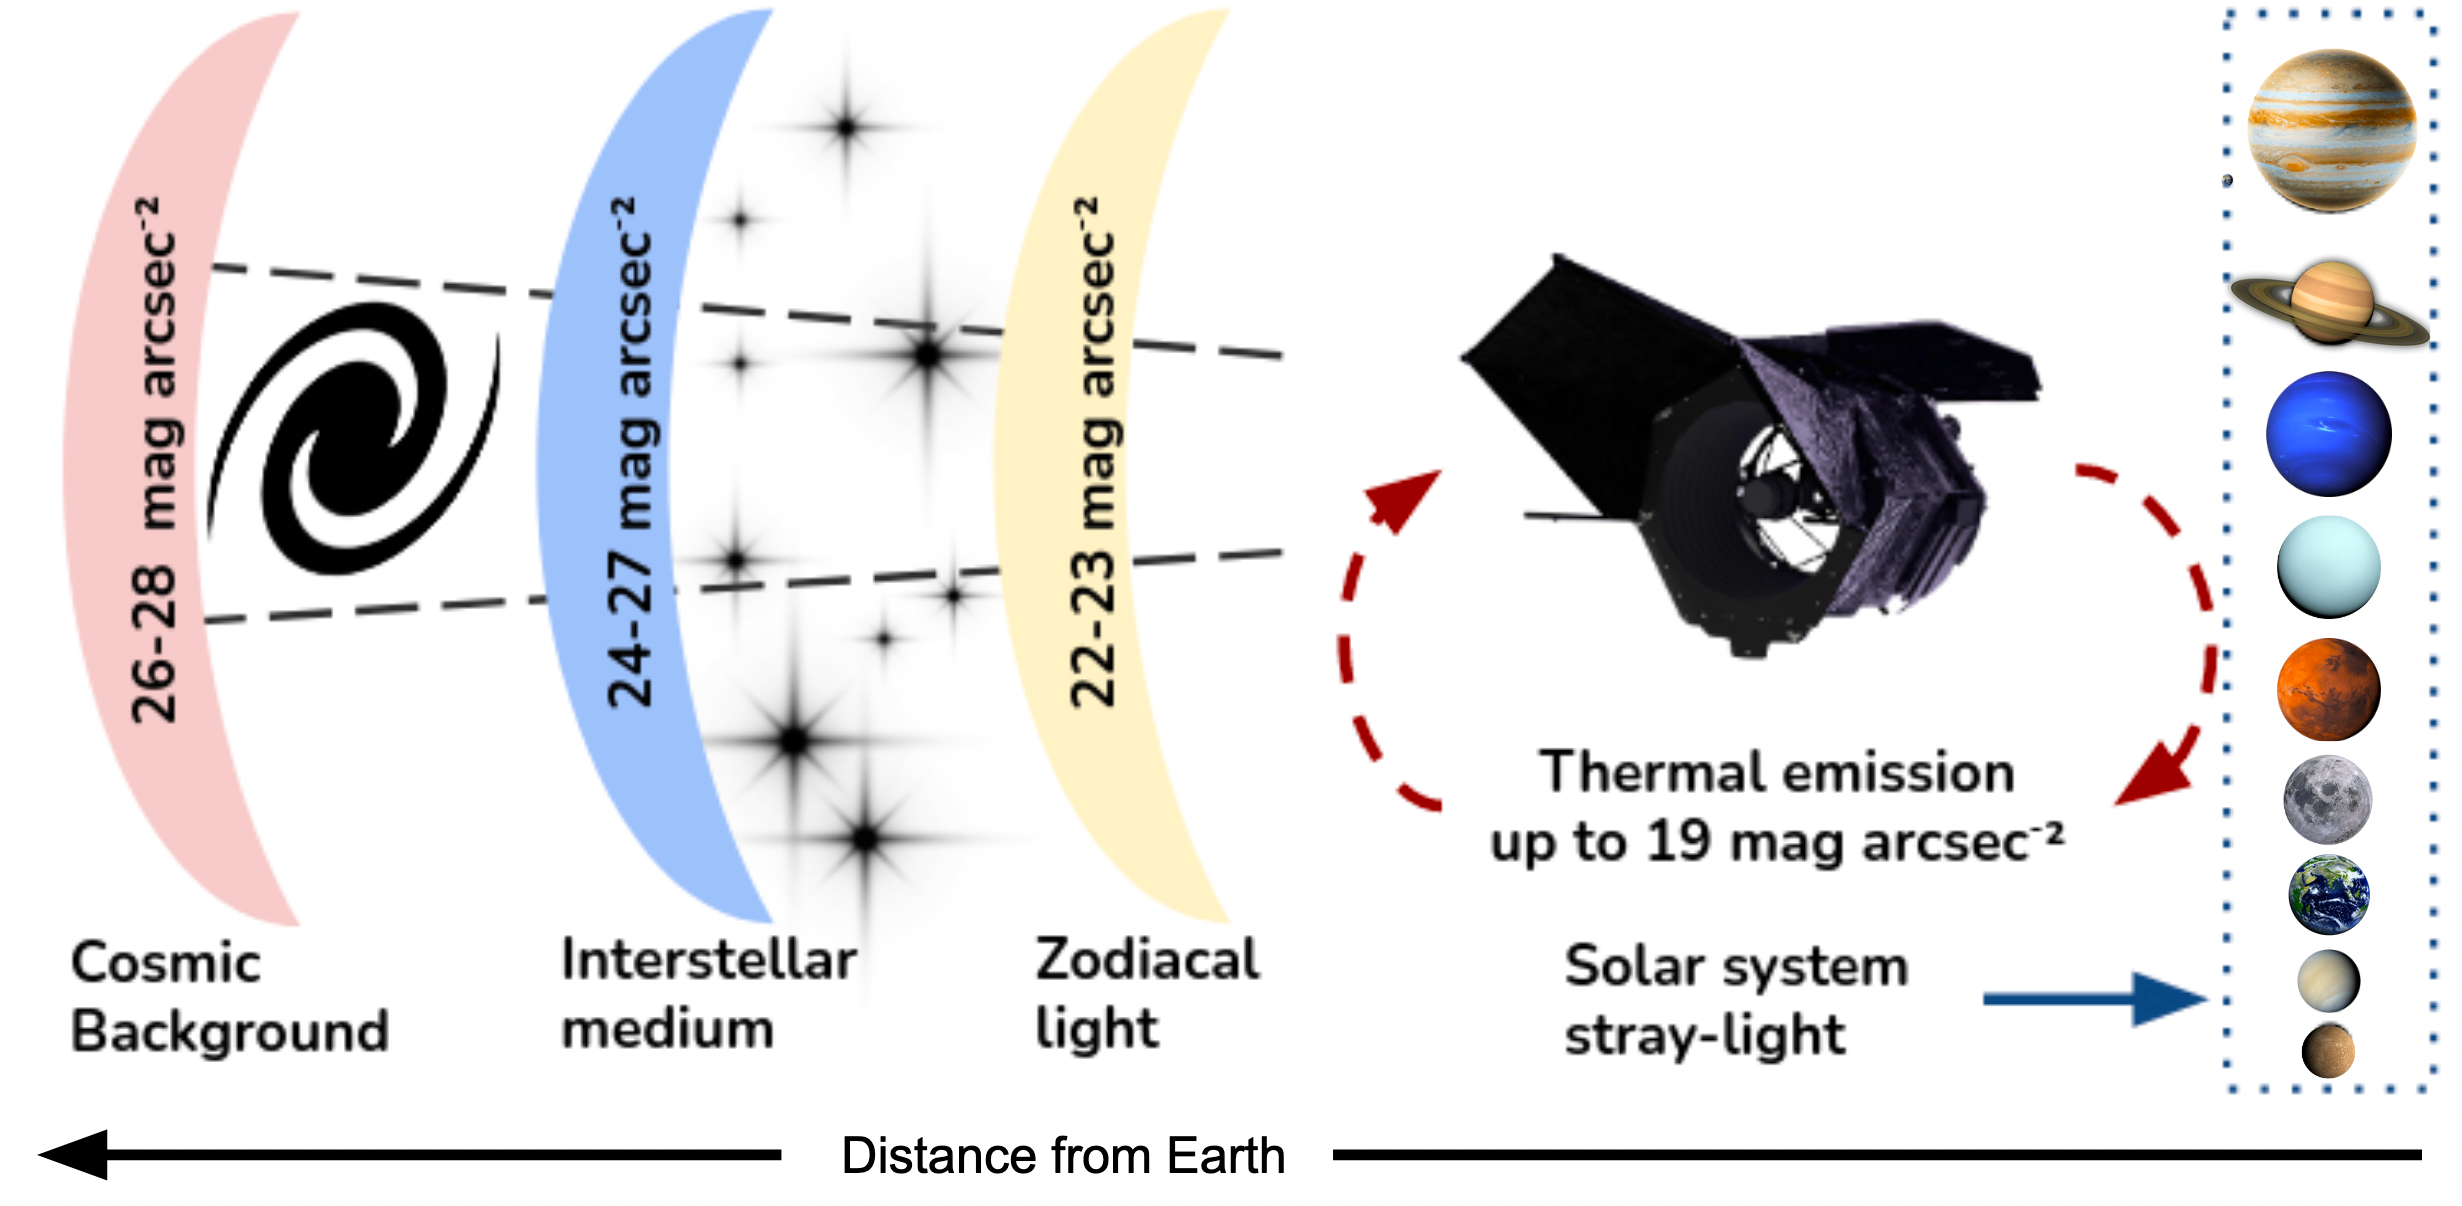
\includegraphics[trim={0 0 0 0}, clip, width=0.6\textwidth]{roman_scheme.png}}
  \raisebox{-0.5\height}{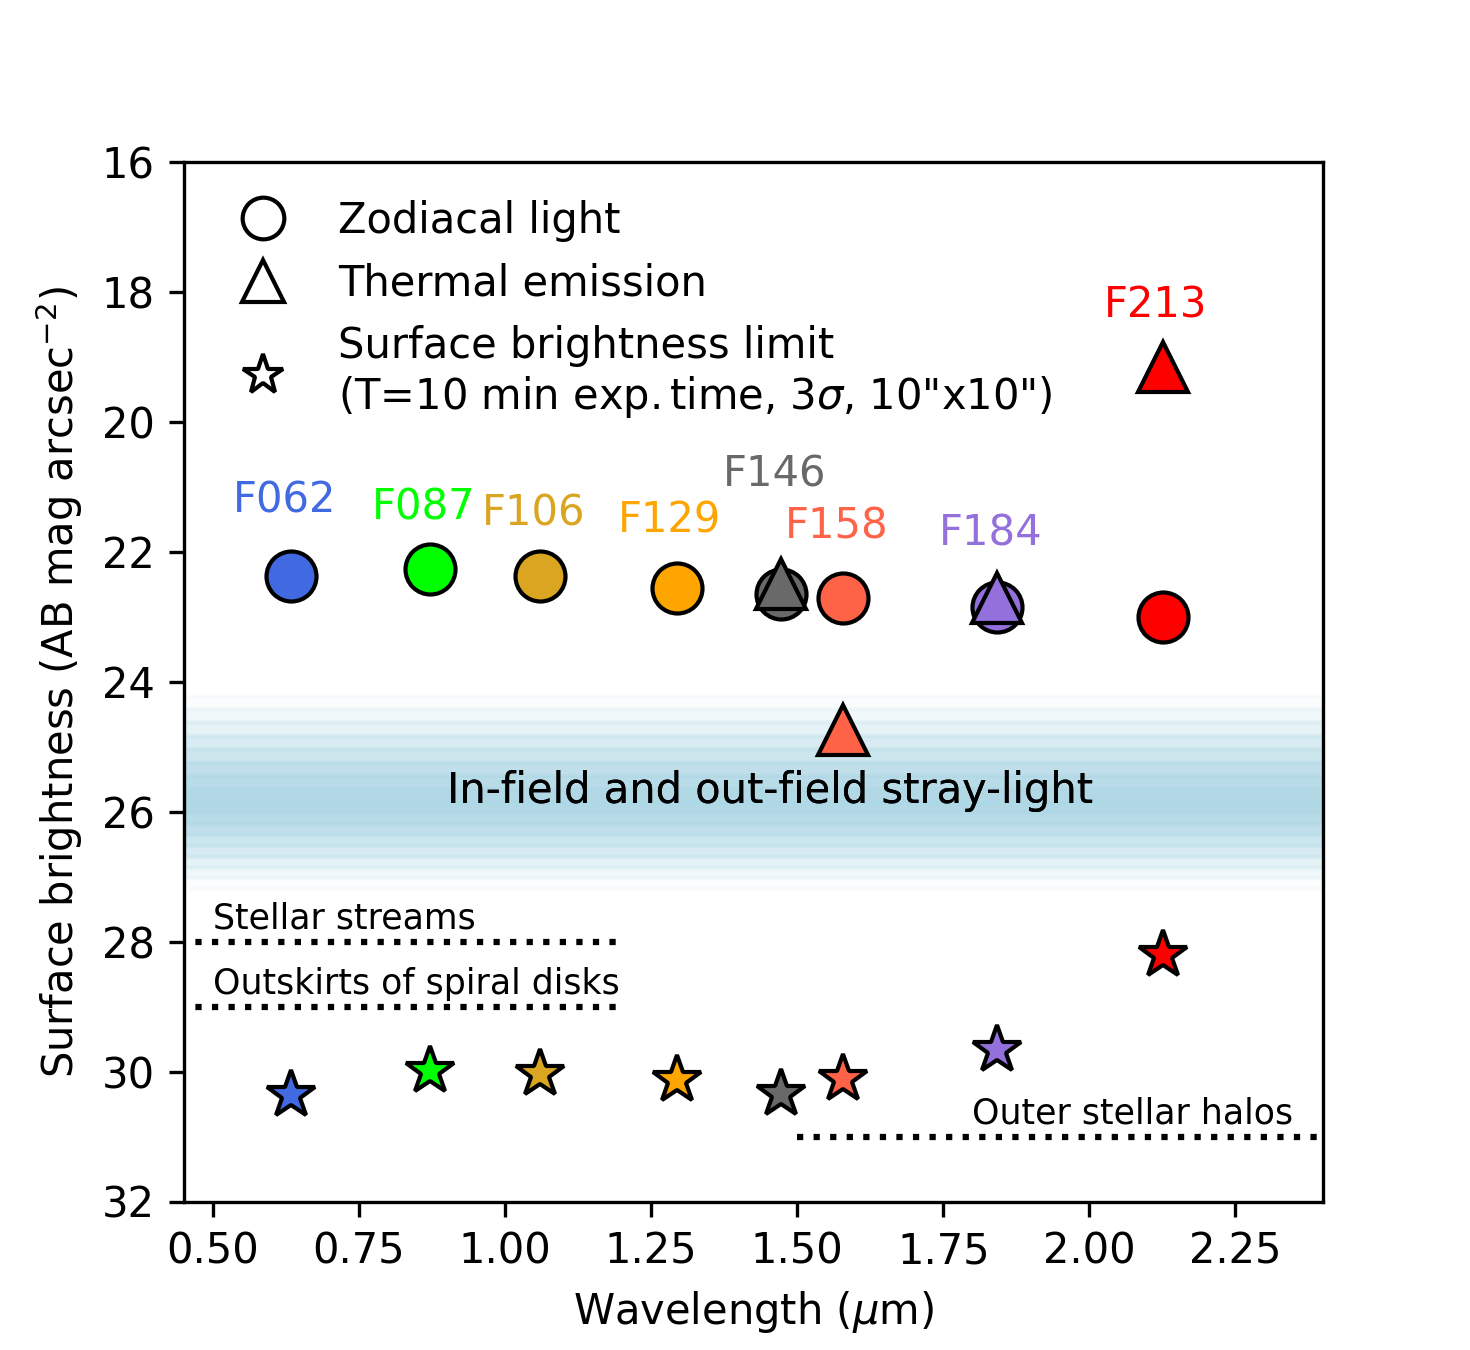
\includegraphics[trim={0 0 30 0}, clip, width=0.39\textwidth]{roman_filter.png}}
\end{minipage}
\caption{Background emission for \RST/WFI. \emph{Left:} The sky background of WFI will be a combination of Zodiacal light, Milky Way interstellar emission, Cosmic Background --CIB--, stray-light from stars and Solar System objects, and thermal emission from the spacecraft. \emph{Right:} Zodiacal light, thermal emission, and stray-light (based on \emph{Euclid} estimates) surface brightness for the \RST/WFI filters, compared with the expected surface brightness limit. Zodiacal light dominates the background except in the F184 and F213 filters, where thermal emission starts to dominate.}
\label{fig:roman_background}
\end{center}
\end{figure*}
Despite their advantageous position above the atmosphere, space telescopes are sensitive to a large number of sources of light contamination. Photons that reach the detector out of their intended optical paths (stray-light) can be a potential source of light contamination, generating artificial systematic gradients, increasing background level, and ultimately affecting the limit of detection of certain astronomical sources \citep{borlaff+2019aap621_133}. \texttt{ROSALIA} is the first attempt to characterize layer by layer the background on astronomical images obtained from space, focusing on the stray-light background on \RST/WFI images at very large spatial scales (several arcmins to the complete FOV). The presented tools (\texttt{ROSALIA}) based on ray-tracing simulations serve as a correction of low surface brightness sky background gradients at very large spatial scales in individual exposures of the \RST\ Wide Field Instrument. 


\section{Methods} \label{sec:methods}

Astronomical sources (i.e., galaxies) are generally identified over a smooth background of photons (sky background) by subtracting a fitted surface to pixels unassociated with the source from the science image. While this technique is useful for point source photometry, it is not valid for very dim extended sources, given the significantly higher challenge in identifying surrounding pixels free of source emission. Deep mosaics are composed of many individual images with shorter exposure times, and the extended envelopes of low surface brightness objects are several times dimmer than the noise level. If an observer fits and subtracts a surface to those ``sky-dominated'' pixels, the modeled background will systematically include any undetected dim extended signal and, thus, extremely dim extended sources will be removed in the final mosaic \citep{akhlaghi+2015apj220_1}.\\

%%% Awesome figure Alejandro!

We propose a different approach to remove the sky-background: Instead of fitting a free-shaped surface to the background, we can use the information from the different sources that compose the sky as well as the technical specifications of \RST/WFI to model each layer of the background in a physically-motivated, forward-modeling way, and then subtract the layers (Fig.\,\ref{fig:roman_background}). For an optical/IR telescope like \RST\ pointed at the sky location ($\alpha$, $\delta$) with wavelength $\lambda$ and a given time $t$, the components of an image $I$ are:
\begin{equation}
    I = S(\alpha, \delta, \lambda) + \zeta(\alpha, \delta, \lambda, t) + \beta(\alpha, \delta, \lambda) + \Sigma(\alpha, \delta, \lambda) + \gamma(\alpha, \delta, \lambda) + \Theta(\lambda)
\label{eq:background}
\end{equation}
where $S$ is the signal from astronomical sources of interest (i.e., galaxies, stars), $\zeta$ is the Zodiacal light, $\beta$ the Cosmic optical and infrared background (hereafter CIB), $\Sigma$ is the stray-light (from inside and outside the FOV), $\gamma$ is the emission from Milky Way galactic dust cirri, and $\Theta$ is the thermal background emission of the spacecraft, which can be significant for the longer wavelength filters (up to $\mu_{\rm{thermal}}=19$ \magarc, see Fig.\,\ref{fig:roman_background}). While these layers depend on the sky position and wavelength, the Zodiacal light emission exceptionally also depends on time ($t$, due to the relative Sun angle), and the thermal emission is expected to be only a function of wavelength and position on the FOV. Our approach is the following: $\beta$, $\zeta$, and $\Sigma$ can be accurately modeled in each individual image, thanks to NASA/IPAC Infrared Science Archive (IRSA), \emph{Gunagala}, and \emph{Zodipy} sky background models, the \emph{Gaia}, 2MASS, and WISE point source catalogs, and the optical design of \RST/WFI. The galactic cirri ($\gamma$) will be structurally decomposed from the images based on ancillary IR observations \citep[][Sanchez-Alarcón et al. in prep.]{2025ApJ...979..175L}. By monitoring \RST's thermal stability,  $\Theta$ will be modeled based on the models generated during TVAC testing.

\begin{figure*}[t!]
 \begin{center}
 % trim left bottom right top 
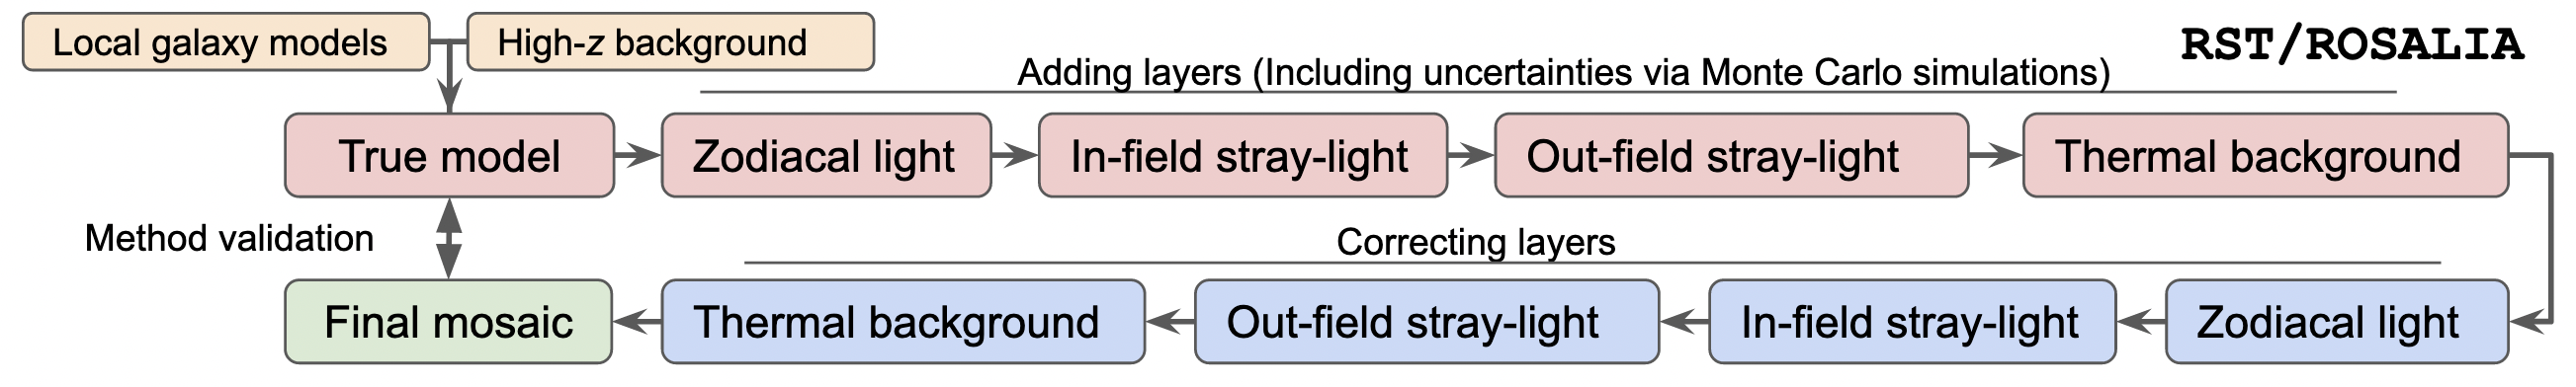
\includegraphics[trim={0 0 0 0}, clip, width=\textwidth]{rosalia_flowchart.png}
\caption{\texttt{ROSALIA} project flowchart: \emph{Orange:} Input \emph{True Universe} models. \emph{Red:} Sky-modeling steps, including uncertainties. \emph{Blue:} Simulated calibration. \emph{Green:} Final product. The difference between the final products and the \emph{True Universe} model will serve as testing and validation.}
 \label{fig:flowchart}
\end{center}
\end{figure*}



\subsection{Modeling stray-light from out-of-field sources}\label{sec2:NDI}

The sensitivity to stray-light that a telescope from a contaminating source outside the field of view (FOV) can be described by the Normalized Detector Irradiance \citep[NDI,][]{bely+1991inproceedings_267, bely2003book} function. The NDI is defined as the ratio of the stray-light irradiance (power per unit area) received at the detector to the irradiance of the source at the entrance of the telescope (see Eq.\,\ref{eq:NDI_definition}). This function can be used to estimate the flux of photoelectrons that an off-axis source will generate in a certain region of the detector. Similarly to the Point Spread Function (PSF), the sharpness of the NDI defines the effectiveness of the telescope's baffling. This function is strongly dependent on the optical setup and wavelength. For a given telescope, the NDI depends on the angular distance between the optical axis and the source ($\theta$), the position angle of the source in the focal plane reference frame ($\phi$), the observation wavelength ($\lambda$), and the position on the FOV ($x,y$),

\begin{equation}
\label{eq:NDI_definition}
{\rm NDI}(\theta,\phi,\lambda,x,y) = \frac{E_{\rm stray}(I, \theta, \phi, \lambda, x, y)}{E_{\rm source} (I, \lambda)} \,.
\end{equation}

When the NDI for a certain source is determined as a function of $\theta$, $\phi$, and its position on the FOV is known, it is possible to estimate the stray-light contamination ($S$, e$^-$\,\si{{\rm px}^{-1}\,{\rm s}^{-1}}) created by a source of magnitude $m_{\rm AB}$ that produces an irradiance ($I$, \si{W m^{-2}}) at the entrance of the telescope as:
%
\begin{equation}
\label{eq:straylight_estimation_3}
S(I,\theta,\phi,\lambda,x,y) = {\rm NDI}(\theta,\phi,\lambda,x,y)\,I\,A\,T\, \frac{\lambda_{\rm ref}}{h\,c} \,,
\end{equation}
where $h$ is the Planck constant (\si{kg\,m^2\, s^{-1}}), $c$ is the speed of light (in \si{m\, s^{-1}}), the reference bandpass wavelength (in \si{m}), $T$ is the average transmission of the filter, and $A$ is the physical pixel area expressed in m$^2$. The NDI for a given telescope and instrument can be estimated through a numerical approach by using ray-tracing simulations. 


To simulate the propagation of light through \emph{Roman} Space Telescope, we used FRED Optical Engineering Software \citep[i.e., \texttt{FRED} hereafter,][]{turner2004inproceedings_333}. We first divided each one of the 18 WFI SCAs in $8\times8$ subarrays ($512\times512$ pixels in size). From each one of the 1152 subarrays, we launched $N=10^{10}$ rays in reverse through the observatory. FRED tracks the scattering and reflections on each surface until they escape the telescope, and the angular orientation in the sky with respect to the WFI boresight is recorded. The ratio of the number of rays received per unit angular area in the bounding sphere to the original number of rays gives a direct measurement of the NDI (see Eq.\ref{eq:NDI_definition}). The maps in Fig.\,\ref{fig:NDI_ROIs} represent the average NDI for WFI at two angular scales ($2\times2$ degrees and $20\times20$ degrees).

To measure the total stray-light received per pixel on each exposure we follow the method described in \citet[][]{Borlaff+2022aap657_92}. The \Gaia\ \citep[0.3 -- 1 $\mu$m][]{collaboration+2018aap616_1}, 2MASS \citep[1.2 -- 2.2 $\mu$m,][]{skrutskie+2006aj131_1163} and WISE all-sky \citep[3.4 -- 22 $\mu$m,][]{Wright2010AJ....140.1868W} point source catalogs are used to simulate stray-light produced by stars in optical and infrared bands. Their cross-correlated catalogs provide photometry for 5$\times$10$^8$ objects, plus an extra catalog of 230 very bright stars \citep[not directly observable with \emph{Gaia};][]{sahlmann+2016inproceedings_99042E}. Fluxes in the \emph{Roman}/WFI bands are generated by interpolating the spectral energy distribution to the respective wavelengths. Sources not included in \Gaia, 2MASS, or WISE are predominantly very dim and unlikely to affect the stray-light estimation. Objects close to the FOV ($\theta<10^{\circ}$) are modeled individually while objects at higher angular distances to the FOV can be grouped using a HEALPix cell grid \citep{gorski+2005apj622_759}. Finally, the stray-light contribution of each source to the background is obtained by multiplying by the NDI at their relative distance to each pixel and position angle.
%%%%%%%%%%%%%%%%%%%%%%%%%%%%%%%%%%%%%%%%%%%%%%%%%%%%%%%%%%%%%%%%%%


\section{Results} \label{sec:results}

In this section we describe the selection of simulated exposures used to describe the stray-light backgrounds. We selected two types of models: 1) worst case scenarios and 2) realistic stray-light scenes. The worst case scenarios are specifically selected pointings where a particularly bright target (a planet or a bright star) illuminates a highly sensitive position of the telescope. These are described in Sec.\,\ref{subsec:worst}. The second set of models are randomized stray-light models based on the proposed observations for one of the Core Community Surveys (High-Latitude Wide-Area Survey - HLWAS). These models provide a characterization of the RST/WFI stray-light background level under nominal conditions. The results are described on Sec.\,\ref{subsec:HLWAS}. 

\subsection{Worst case scenarios}\label{subsec:worst}

If a source illuminates the telescope with an orientation associated with a high NDI, we can expect a high stray-light background level. In particular, we consider high sensitive locations not only those with a high NDI level, but those with a high NDI \emph{variability across the detector}. A high spatial variability of the NDI across the field of view is likely to produce steep background stray-light gradients in the images. Stray-light gradients are hard to fit and remove and they can mimic the distribution of real sources, like galaxies or clusters. Generate those models we purposefully orient \emph{Roman} in orientations that illuminate with bright sources those sensitive regions. These worst case models provide a useful catalog to characterize potential residuals under certain \emph{Roman}/WFI conditions that are unlikely, but might affect certain observations. 

\begin{figure*}[hbt!]
 \begin{center}
 % trim left bottom right top 
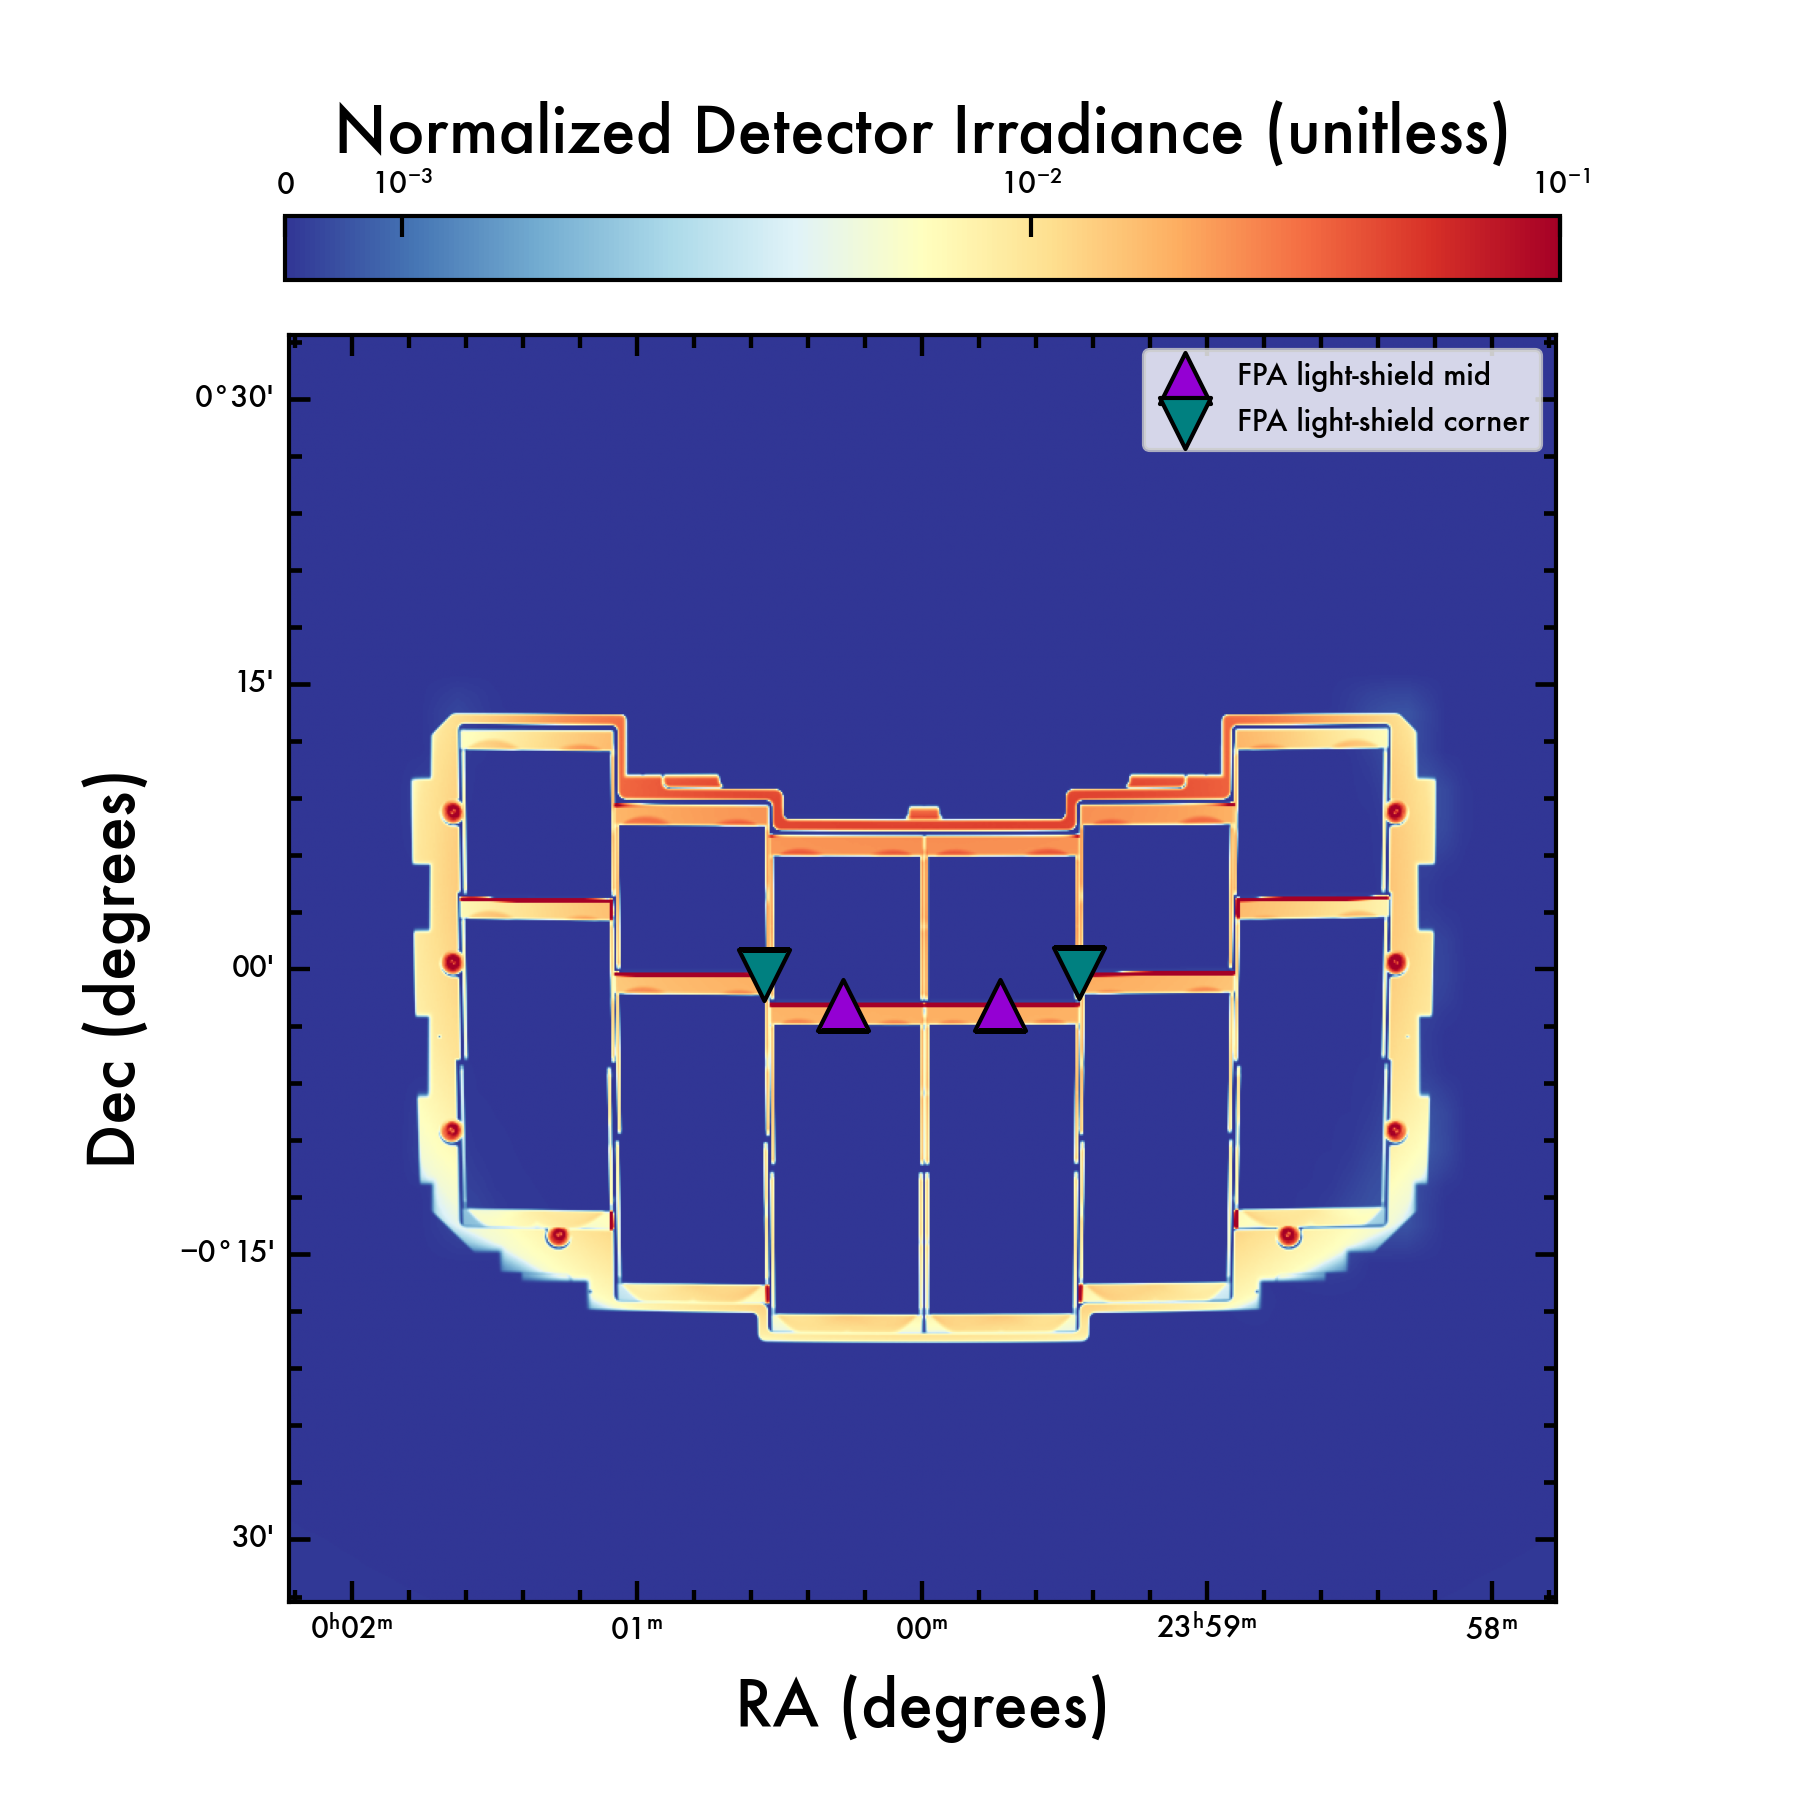
\includegraphics[trim={0 0 60 0}, clip, width=0.495\textwidth]{ndi_2deg_CARs_with_points.png}
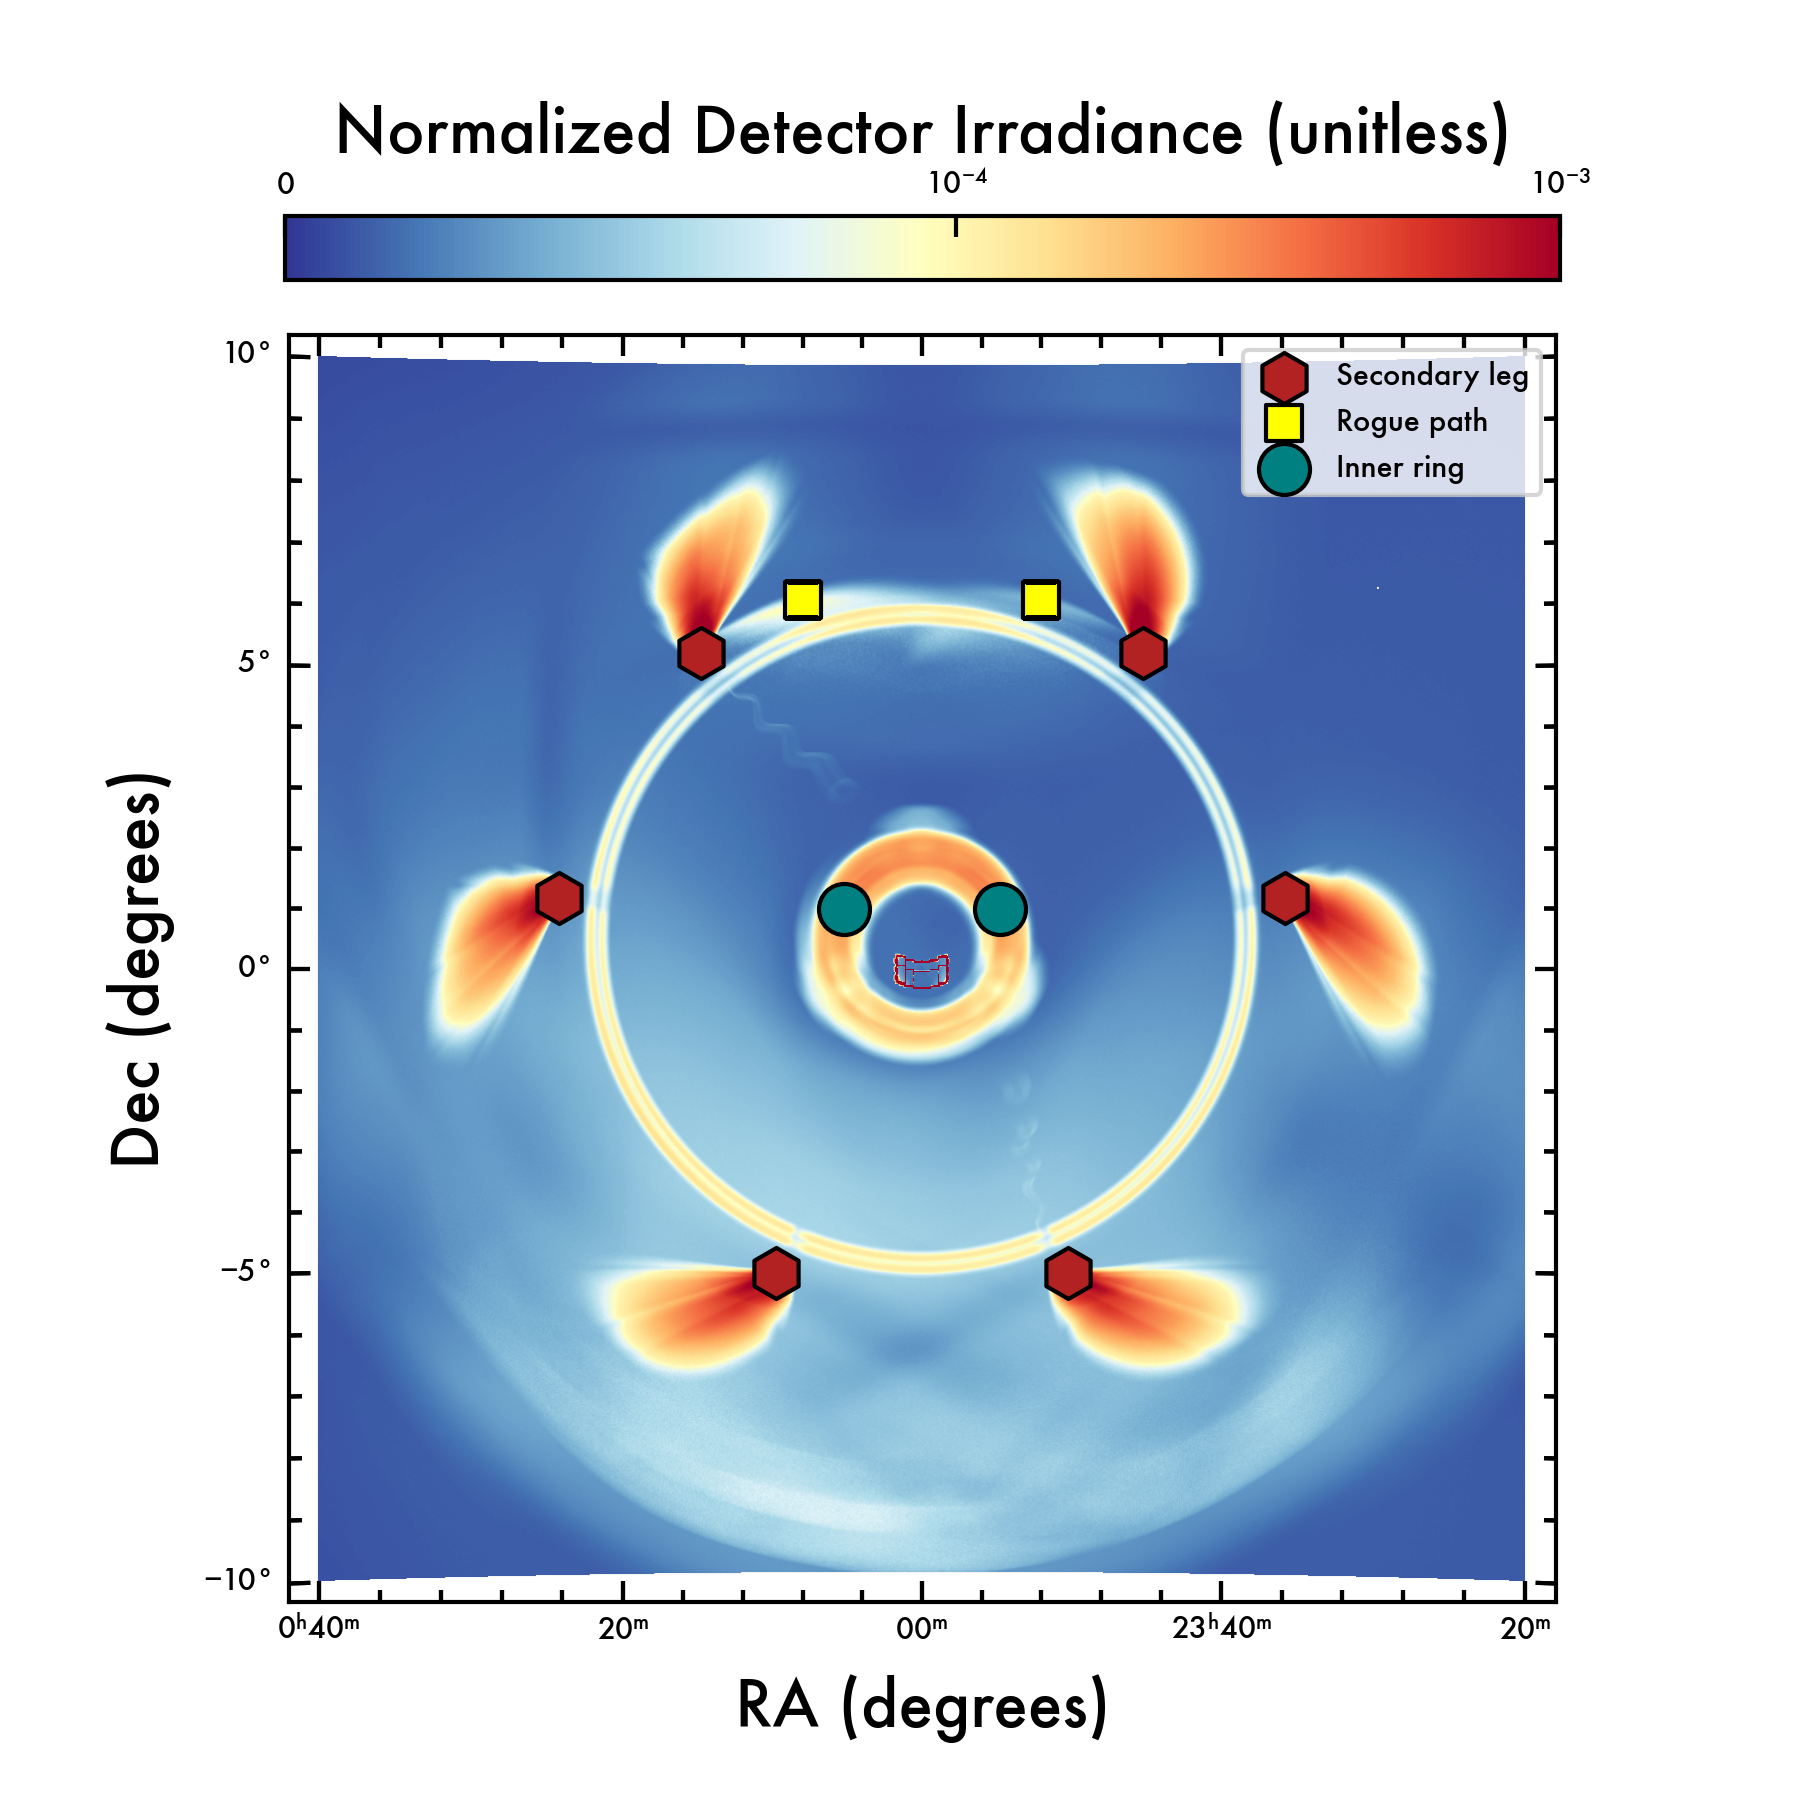
\includegraphics[trim={0 0 60 0}, clip, width=0.495\textwidth]{ndi_20deg_CARs_with_points.png}
\caption{Normalized Detector Irradiance for \emph{Nancy Grace Roman} Space Telescope Wide Field Instrument (WFI), showing the regions of maximum stray-light sensitivity. \emph{Left:} Detail around $2\times2$ degrees from the center of the WFI focal plane. \emph{Right:} Zoom out on the NDI map, extending up to $20\times20$ degrees. Notice the six secondary mirror struts and the shape of WFI focal plane in the center.} 
\label{fig:NDI_ROIs}
\end{center}
\end{figure*}

We identify those stray-light sensitive regions by evaluating the maximum difference between all the NDI maps generated across the field of view. There are five regions of interest described in Fig.\,\ref{fig:NDI_ROIs}. Near the detectors, the sensitivity to stray-light tends to be maximum, as expected. In particular, the edge of the light-shields under SCAs 1, 4, 7, 10, 14, and 16 presents a high NDI value over a thin (10 arcsec) region. This region would be responsible for light anomalies similar to the \emph{Dragon's breath} in \emph{Hubble} Space Telescope ACS \citep{fowler+2017misc} or JWST's claws and wisps \citep{rohrbach+2016inproceedings_99470K}. To illustrate the impact of illuminating this region, one example is shown in Fig.\,\ref{fig:NDI_Dragon_breath}. For this test scenario, we positioned Mizar ($\zeta$ Ursae Majoris, $m\sim2$) between SCAs 10 and 11, on top of the light-shield high sensitivity region. The star produces a characteristic distribution of light that spreads over the nearby detectors, with a peak expected surface brightness magnitude of $\mu_{\rm{S}}=16$ \magarc\ and an average of $\mu_{\rm{S}}=22$ \magarc. The non-affected detectors present a surface brightness of $\mu_{\rm{S}}=25$--$26$ \magarc. 


\begin{figure*}[ht!]
 \begin{center}
 % trim left bottom right top 
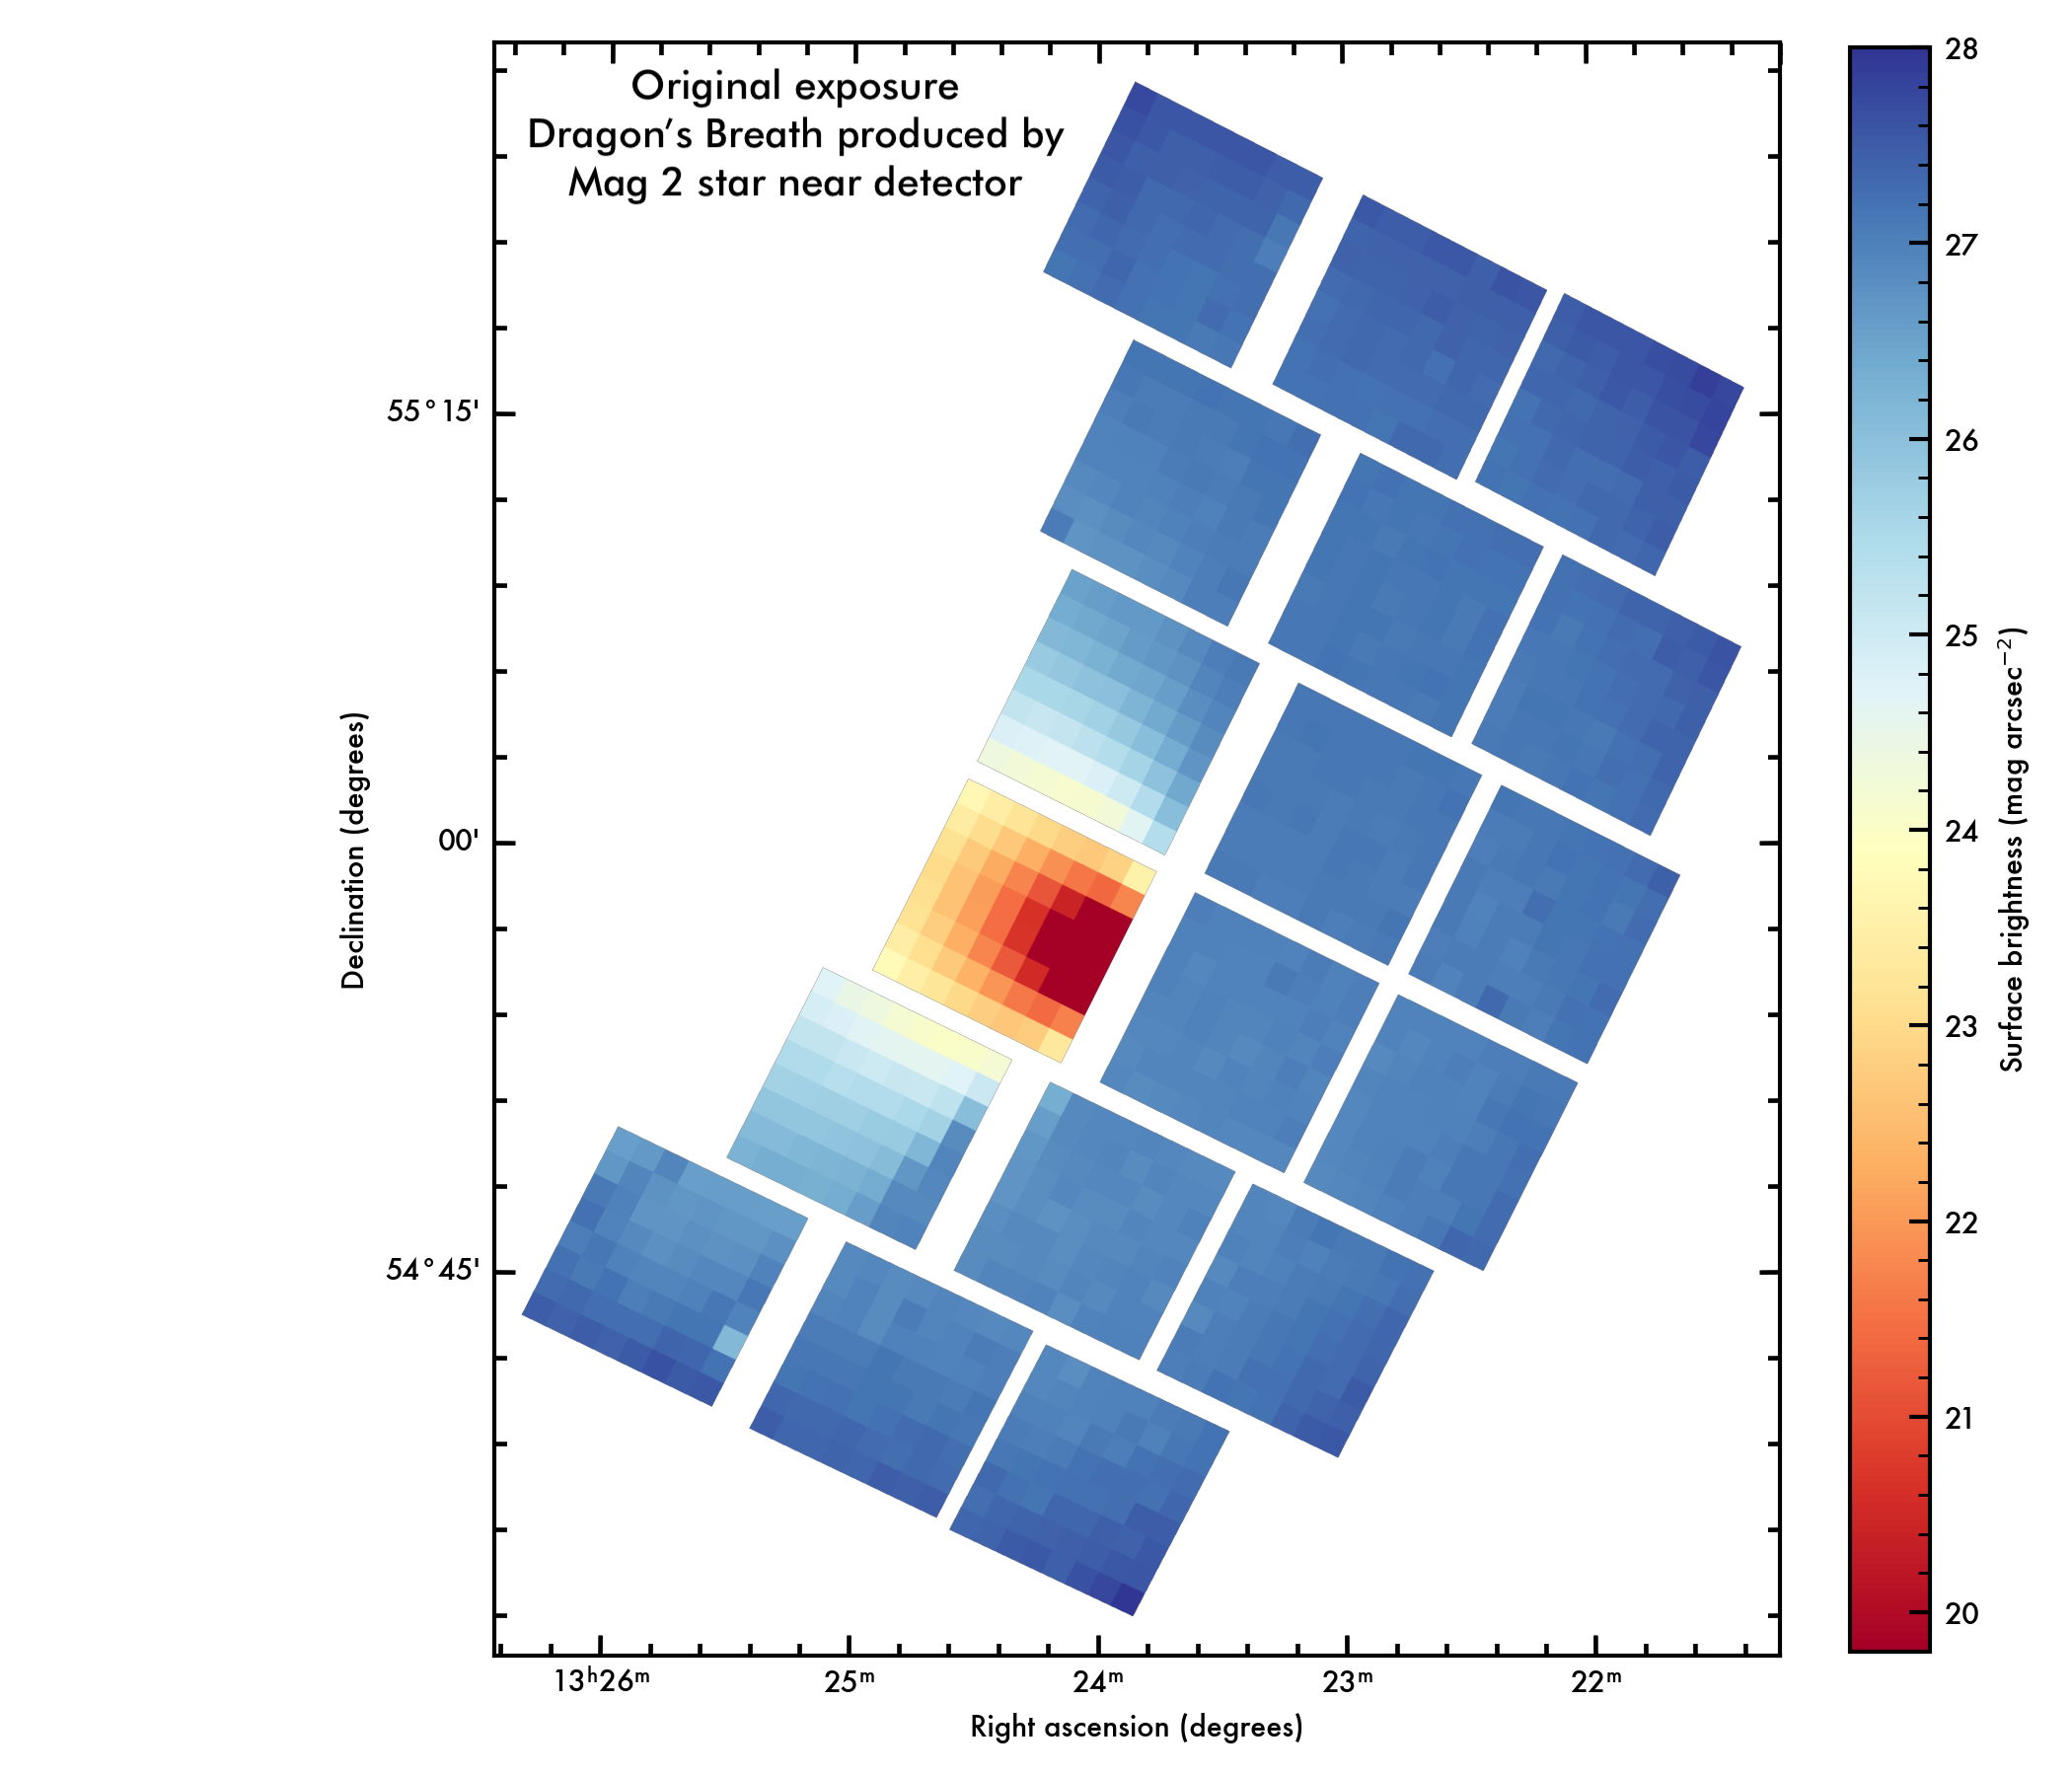
\includegraphics[trim={50 0 10 0}, clip, width=0.465\textwidth]{Dragon_WFI_F129_RA_200.977_DEC_055.001_MJD_61365.00000_PA_063.57_stray_drz_scaled_fe2mu.png}
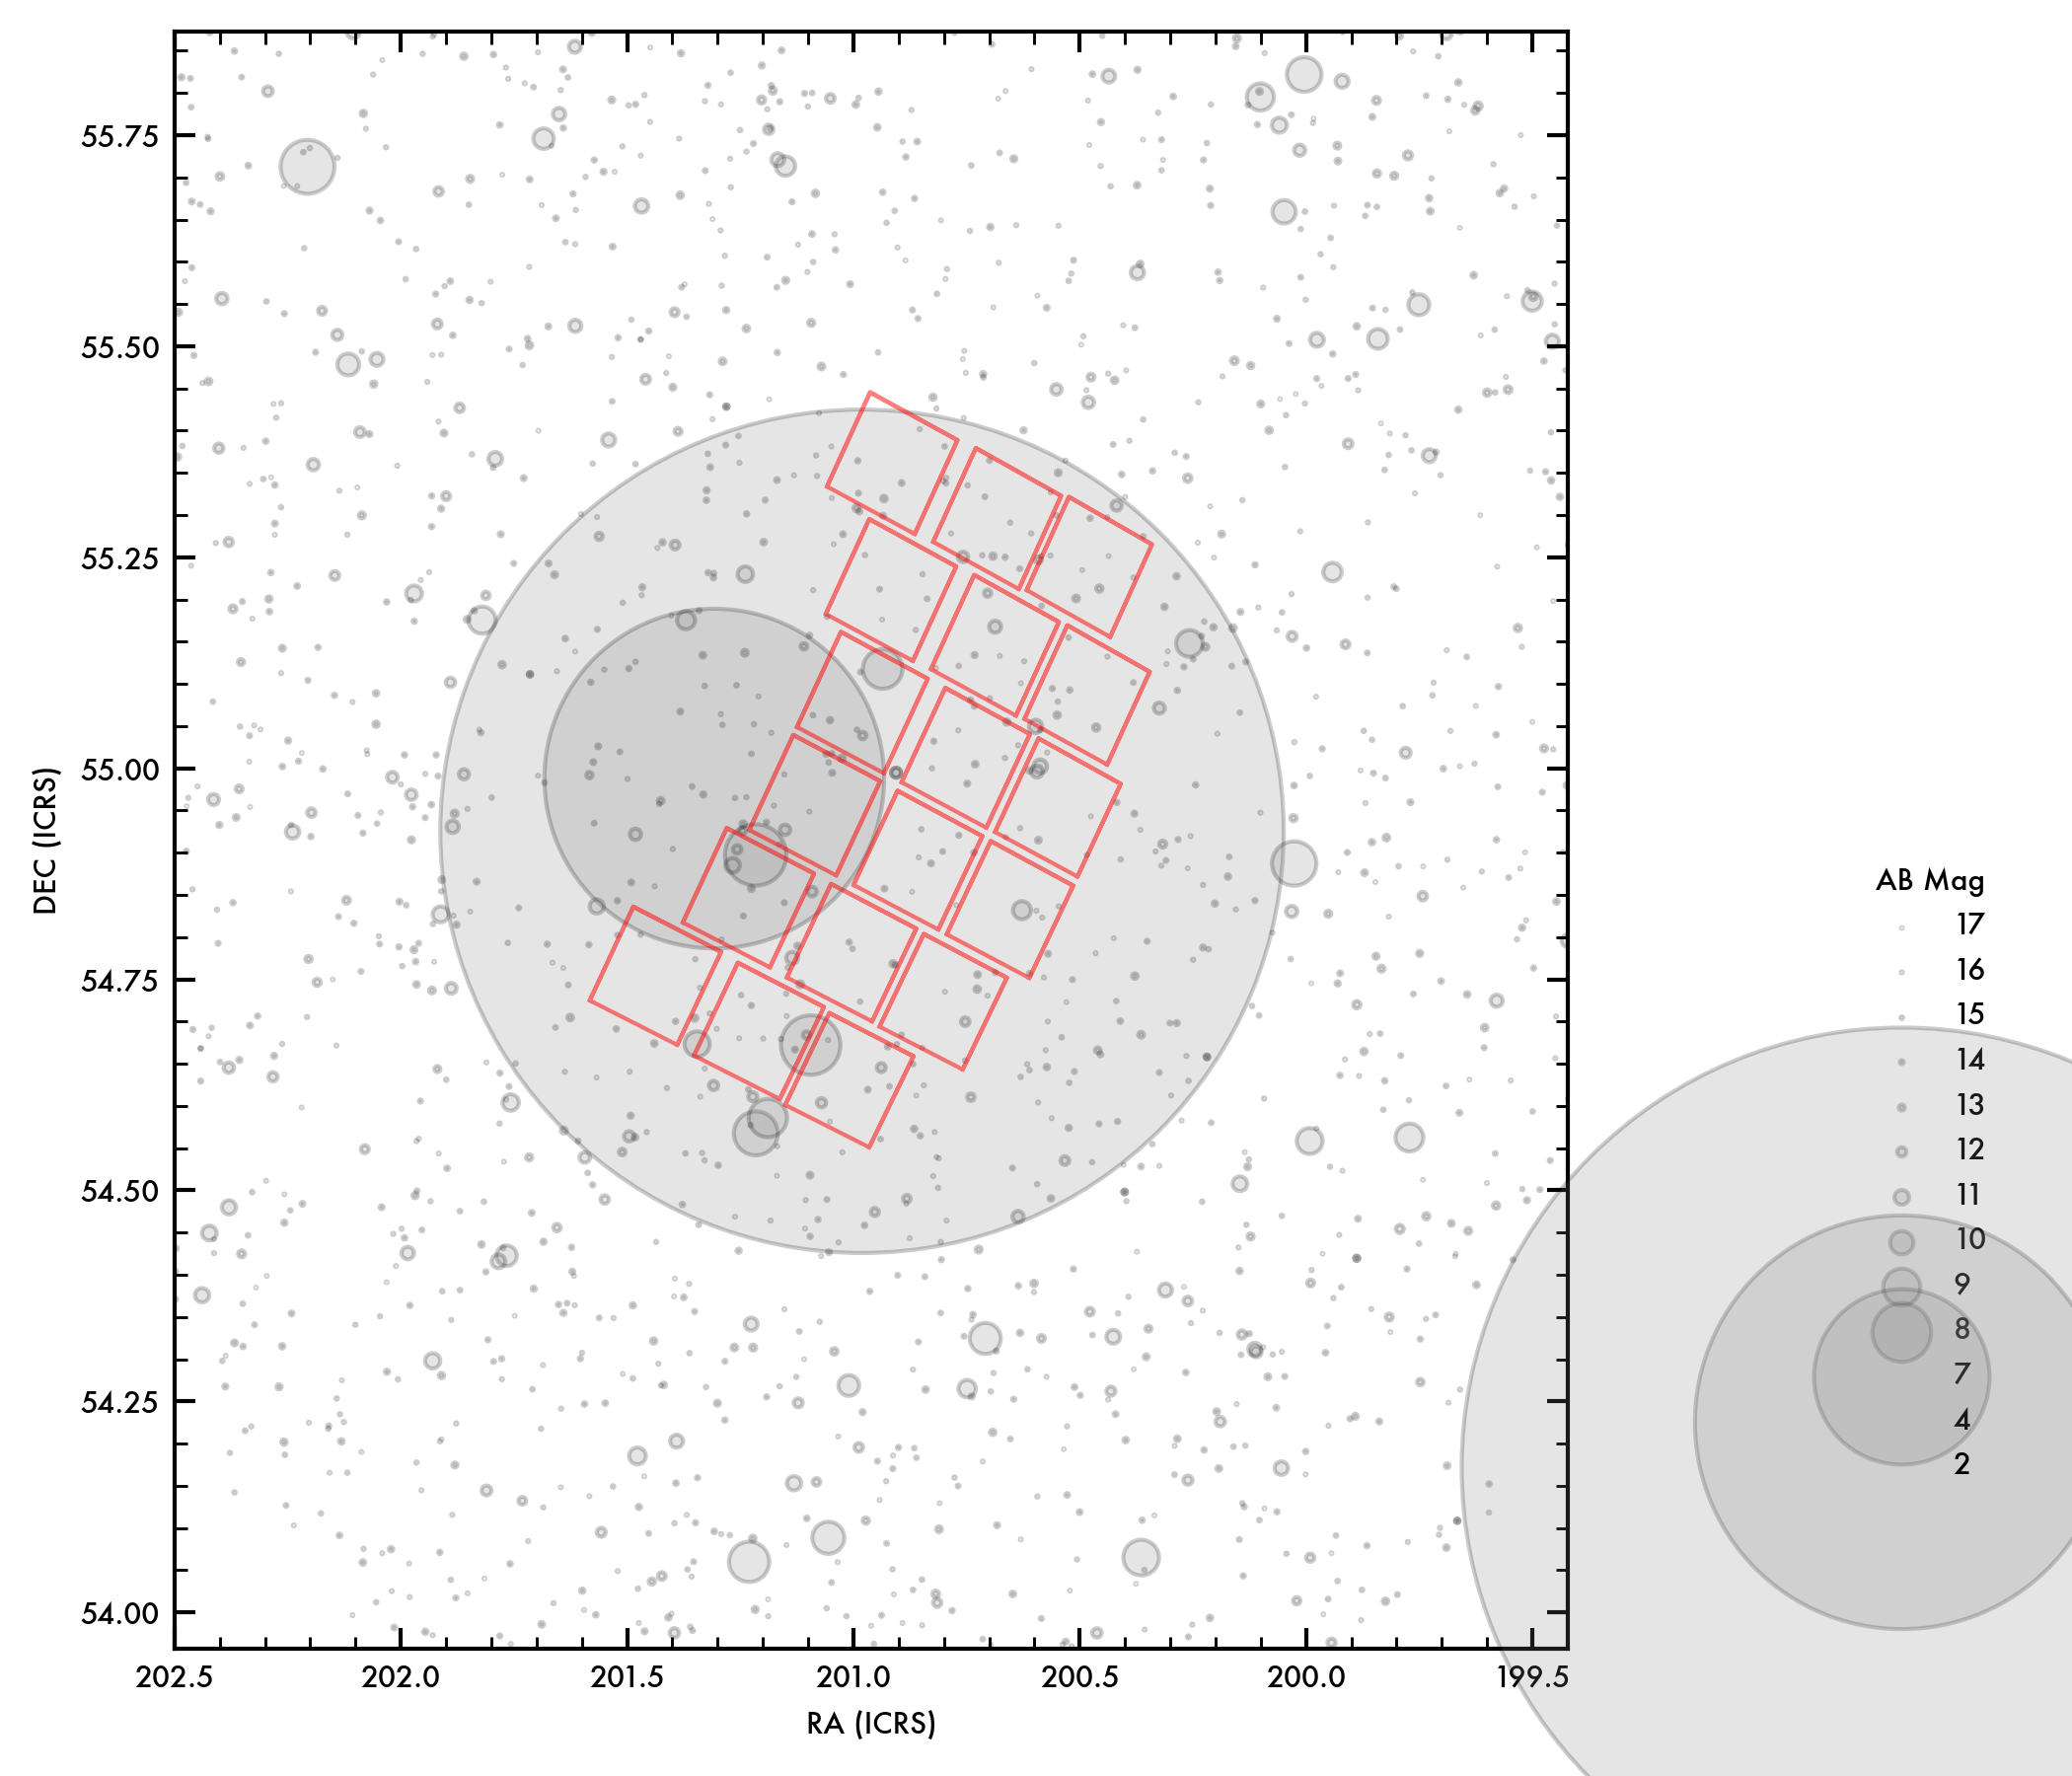
\includegraphics[trim={0 0 0 0}, clip, width=0.525\textwidth]{Dragon_WFI_F129_RA_200.977_DEC_055.001_MJD_61365.00000_PA_063.57_stars_close.png}

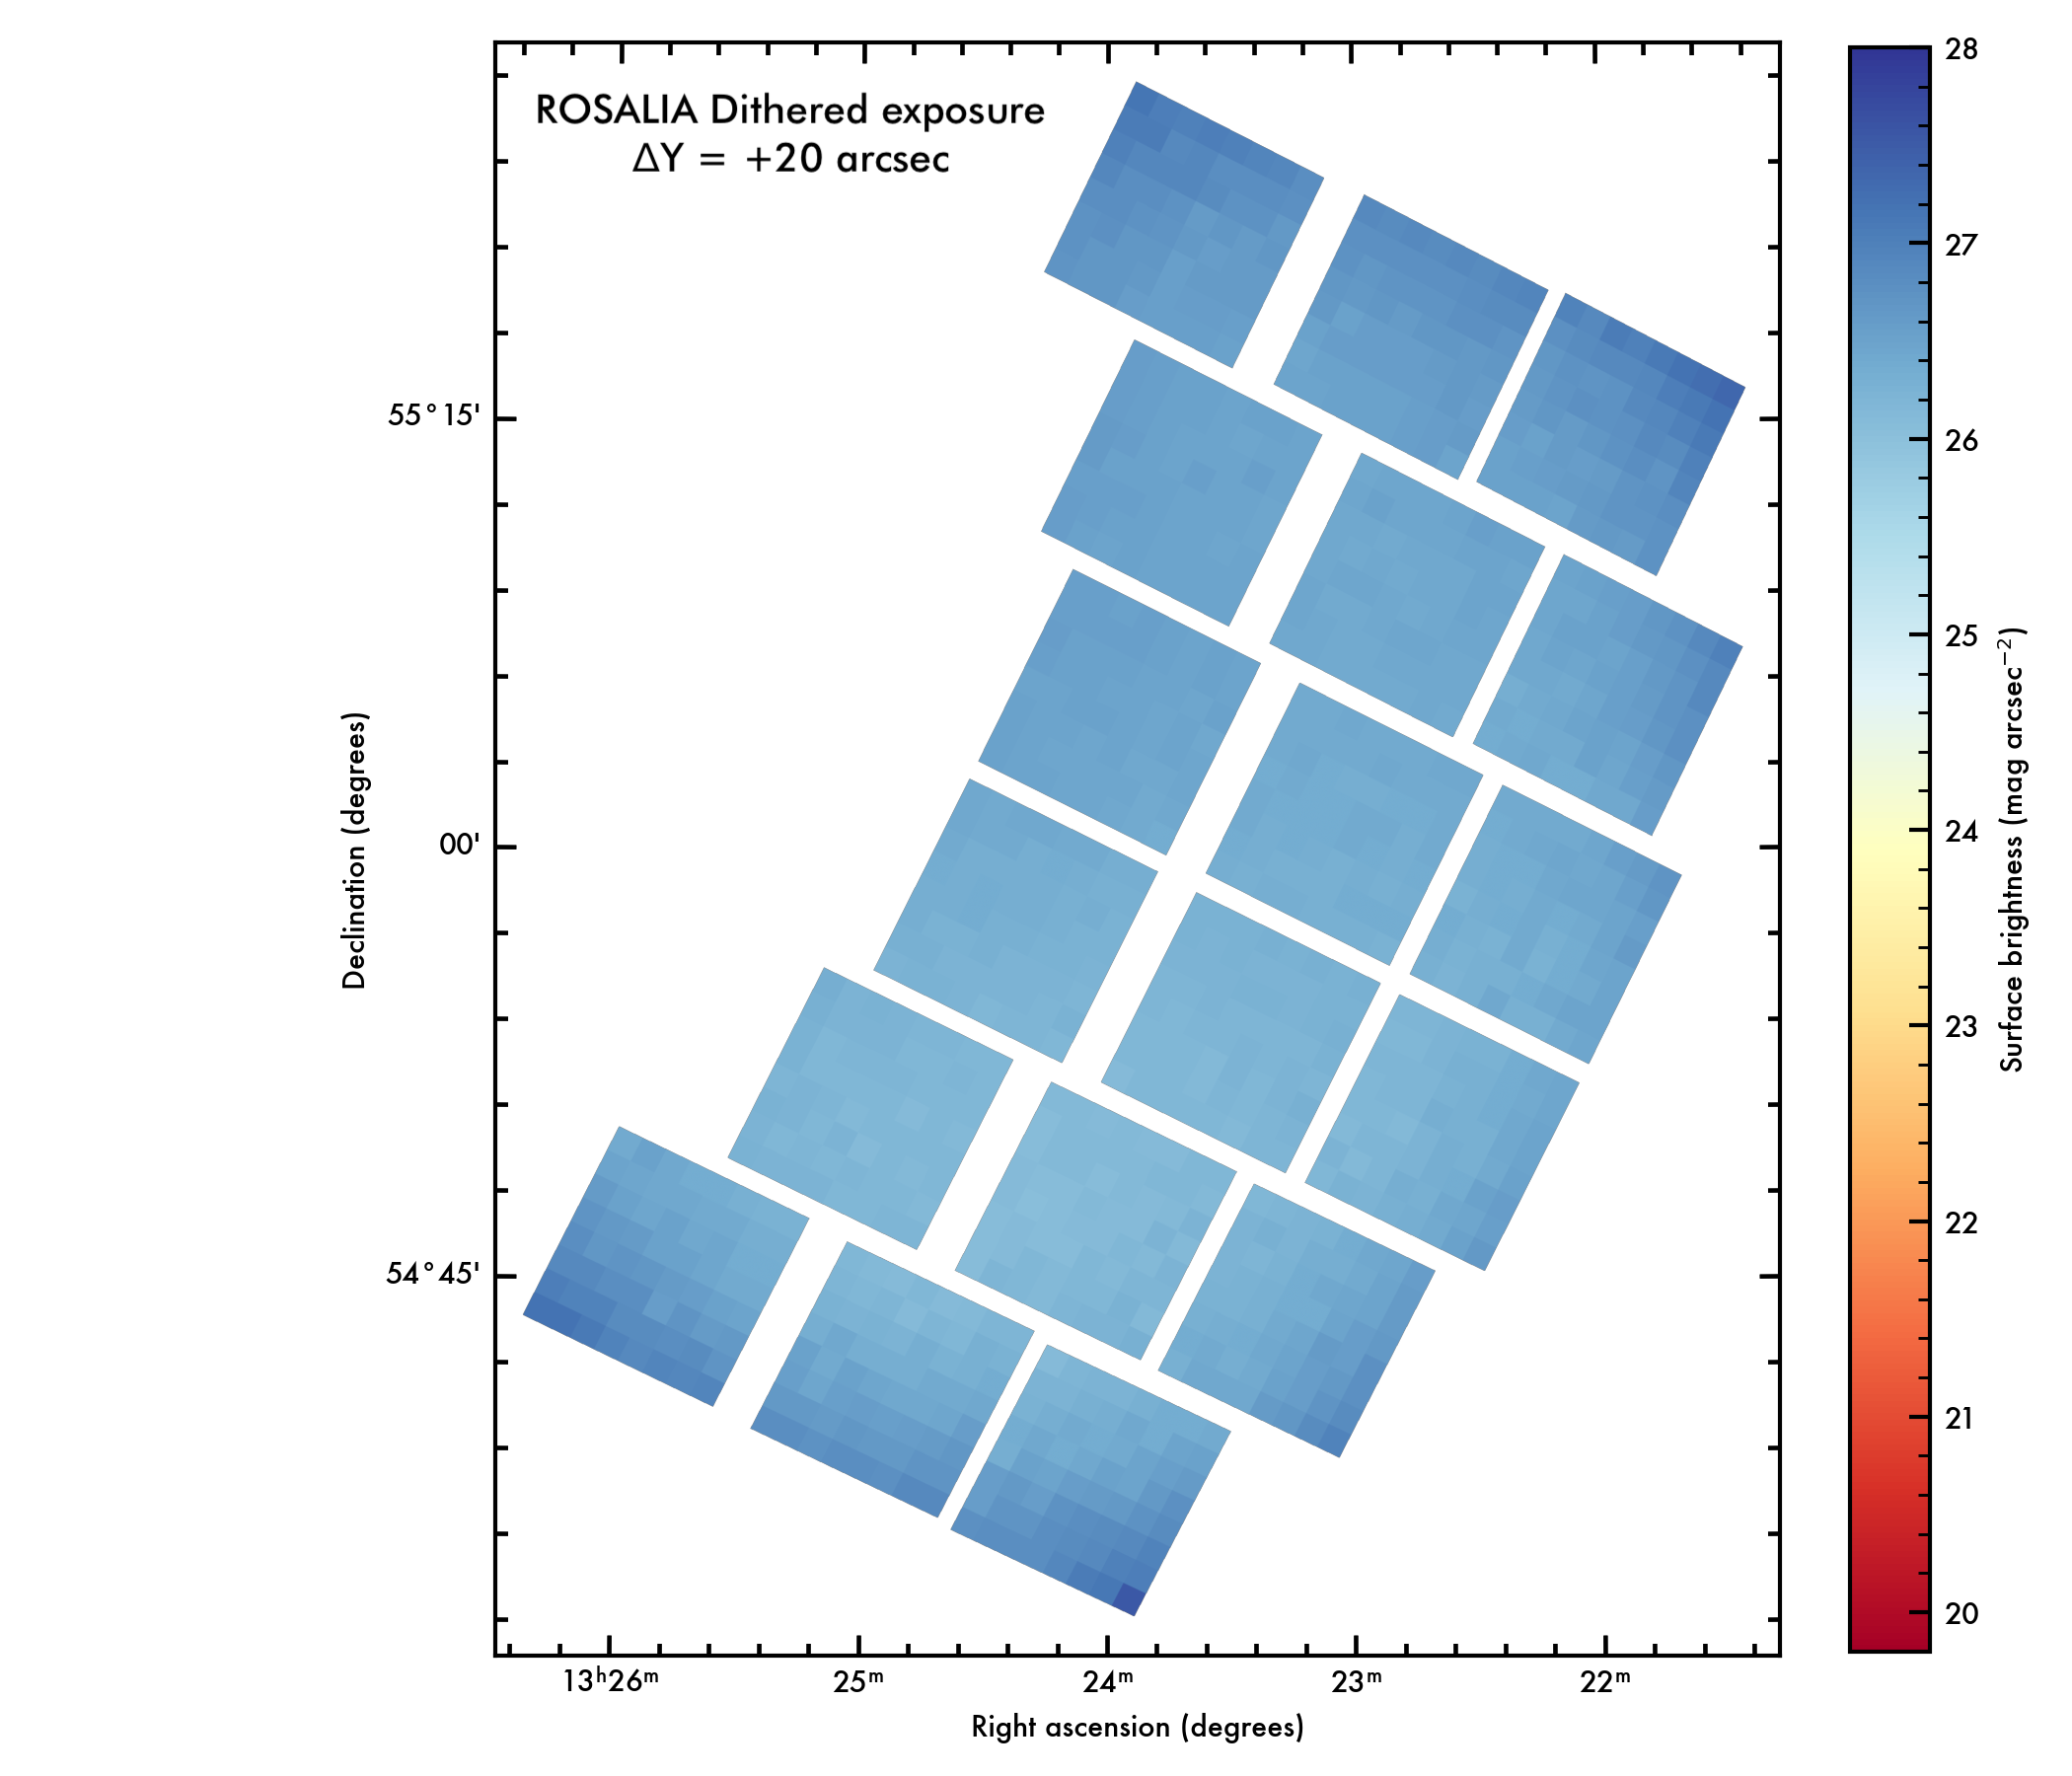
\includegraphics[trim={50 0 10 0}, clip, width=0.465\textwidth]{Dragon_negative_WFI_F129_RA_200.985_DEC_055.003_MJD_61365.00000_PA_063.57_stray_drz_scaled_fe2mu.png}
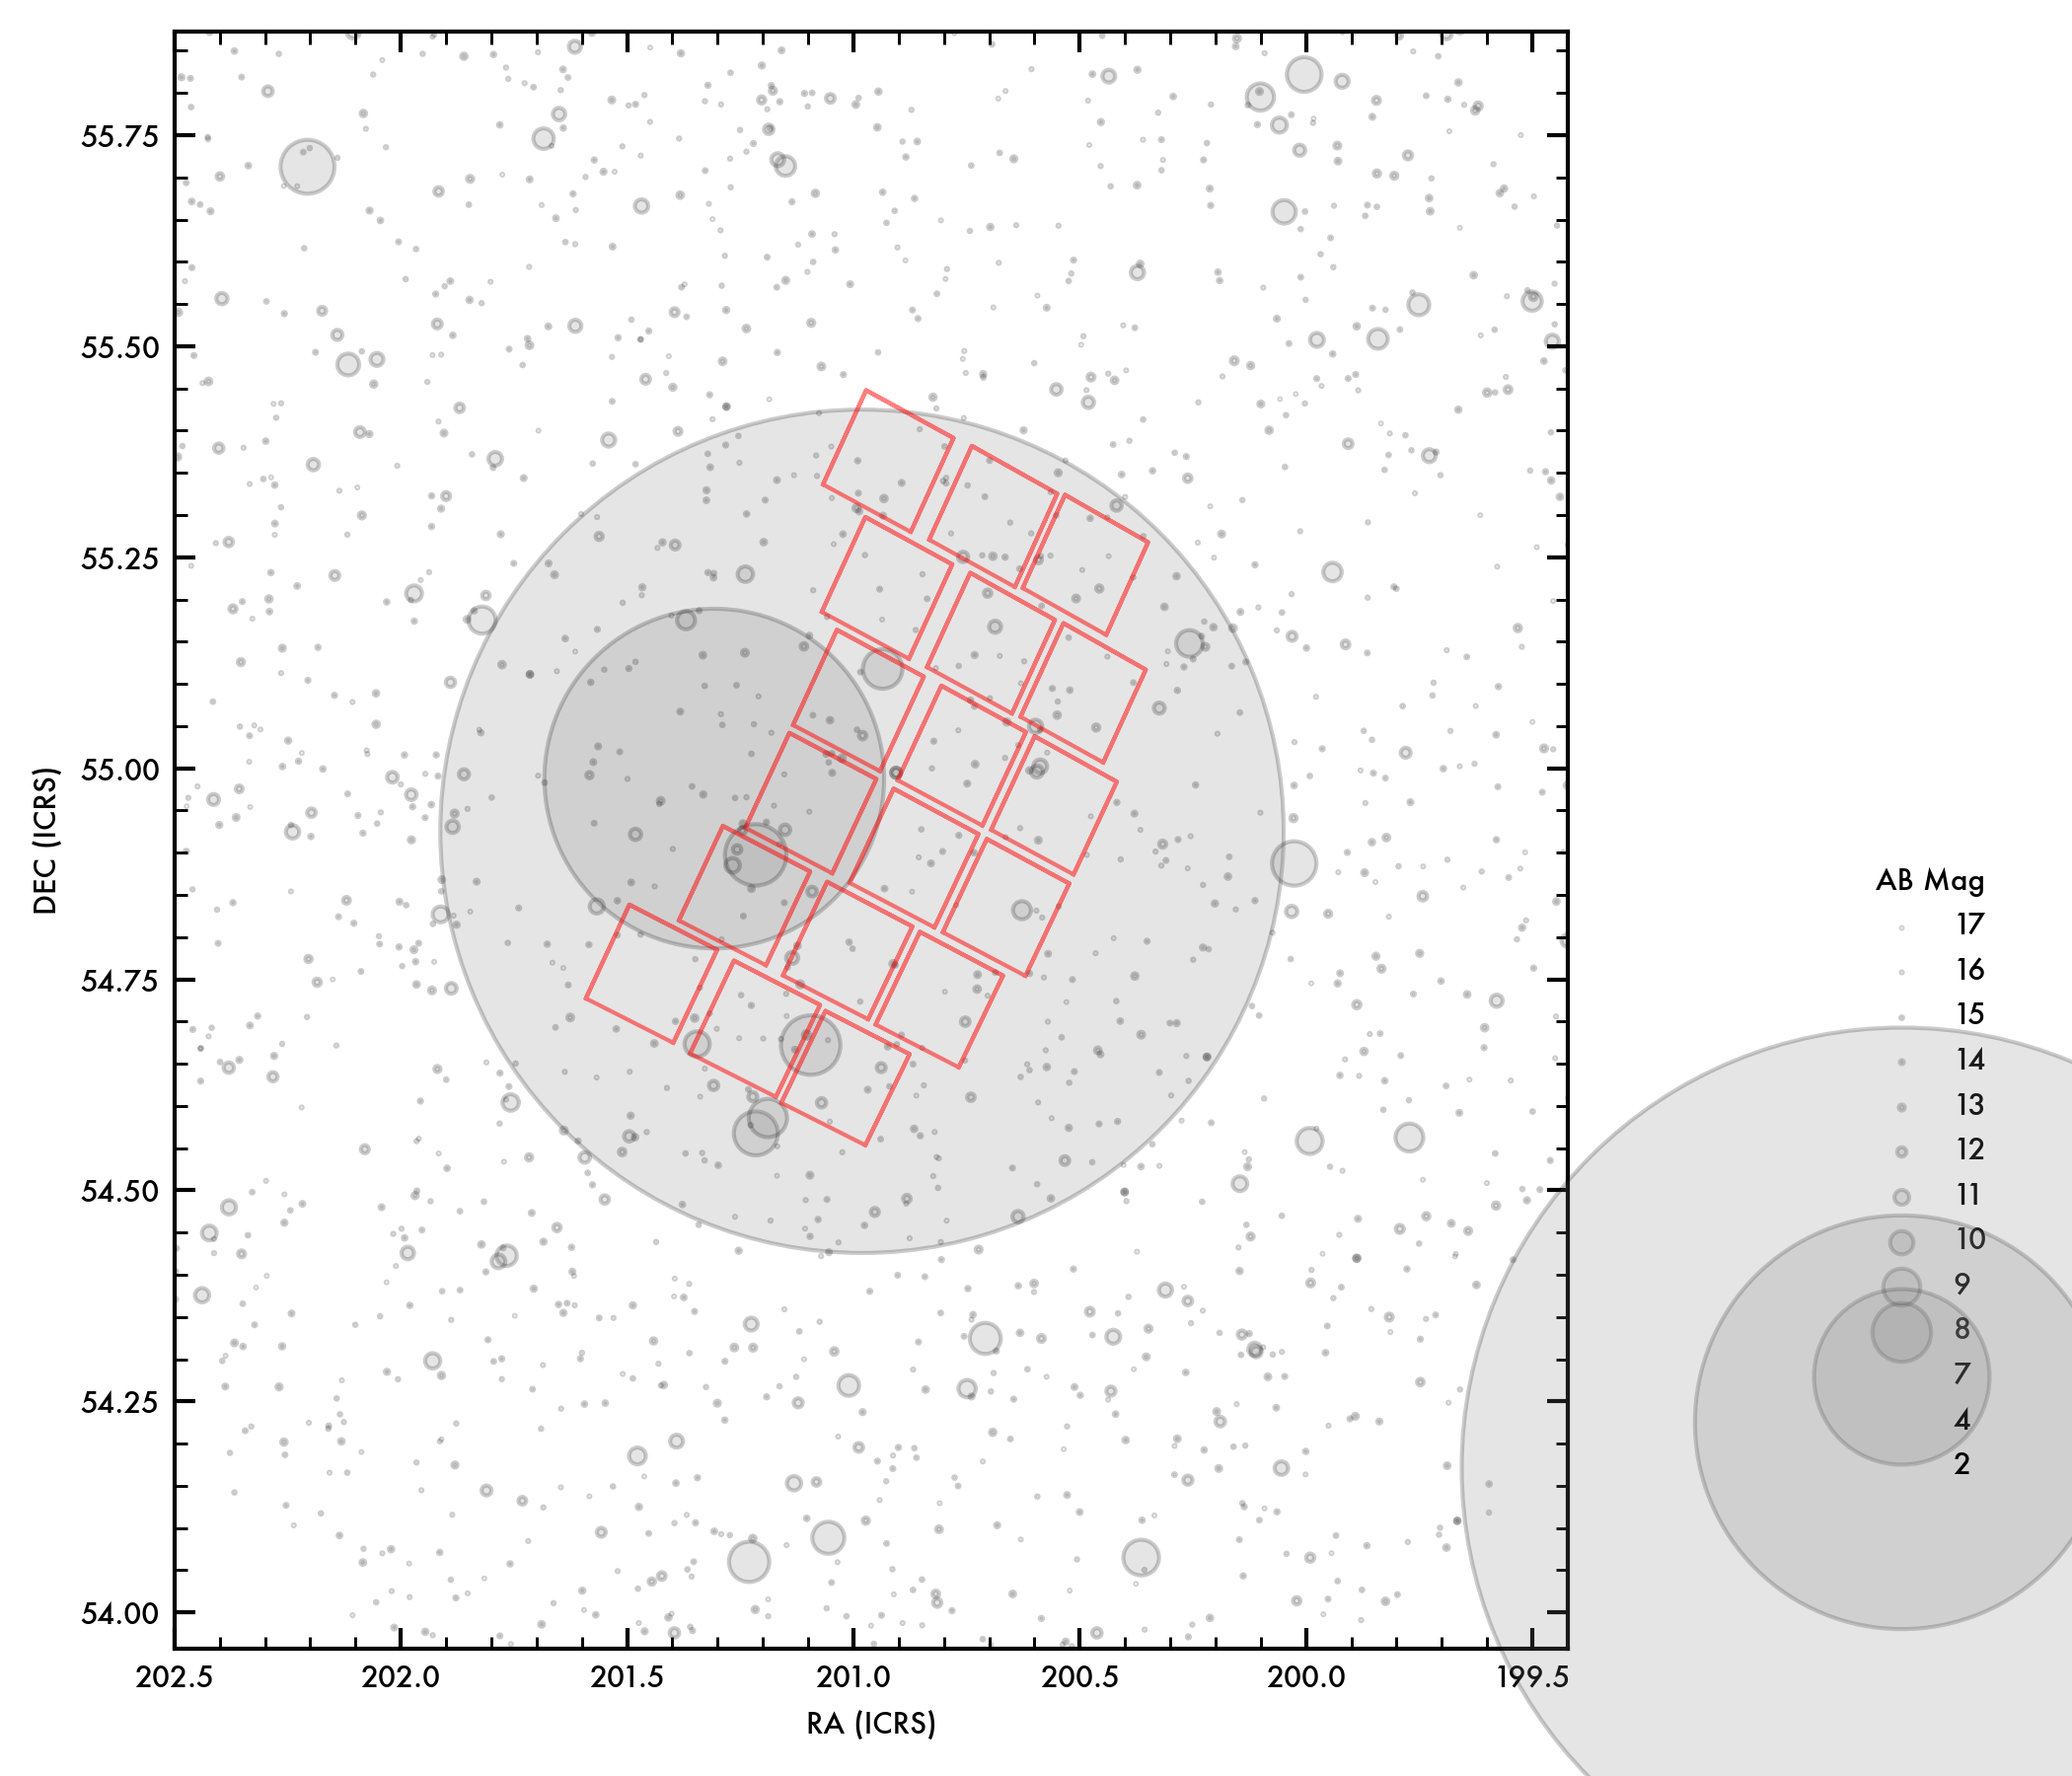
\includegraphics[trim={0 0 0 0}, clip, width=0.525\textwidth]{Dragon_negative_WFI_F129_RA_200.985_DEC_055.003_MJD_61365.00000_PA_063.57_stars_close.png}
\caption{Example of active stray-light suppression using \texttt{ROSALIA} for \emph{Nancy Grace Roman} Space Telescope Wide Field Instrument (WFI). The scene is centered around ($\alpha$,$\delta = 200.985, +55.00$) with the bright star Mizar ($\zeta$ Ursae Majoris, $m=2$). The top row has the star at 5 arcsec from the detector, over the SCA 10 and 11 light-shield gap, representing an extreme example of maximum stray-light sensitivity. \texttt{ROSALIA} predicts that moving the pointing 20 arcsec reduces stray-light from 20 to 26 \magarc. \emph{Top left:} Surface stray-light background, in \magarc. \emph{Top right:} Footprint of the simulated exposure, showing the surrounding stars as circles scaled by flux logarithmically. The largest circle represents $\zeta$ Ursae Majoris ($m=2$). \emph{Bottom row:} Same exposure, displaced 20 arcsec in the -Y detector direction. Notice how the stray-light surface brightness magnitude decreases from $\mu_{\rm{S}}=20$ \magarc to $\mu_{\rm{S}}=26-27$ \magarc.} 
\label{fig:NDI_Dragon_breath}
\end{center}
\end{figure*}

One of the best capabilities of \texttt{ROSALIA} is the ability to dynamically simulate a scene and optimize the background based on the optical information stored about \emph{Roman}/WFI. This methodology allow us to flag regions than might be contaminated by objects outside the field of view. For \emph{Roman}/WFI, the width of the high-sensitivity stray-light region under SCA 10 is less than 10 arcsec. In the example from Fig.\,\ref{fig:NDI_Dragon_breath}, this allows to improve the background levels by including minimal adjusting to the pointing coordinates. The lower row of Fig.\,\ref{fig:NDI_Dragon_breath} represents the same image, dithered 20 arcsec in the -Y direction. In this dithered simulated exposure, the stray-light is drastically reduced from $\mu_{\rm{S}}=20$ \magarc to $\mu_{\rm{S}}=26$ \magarc\ in most of the affected area, including the most affected detector in this case, SCA10. The capability to improve the background level by implementing recommended dithered observations is one of the core functionalities of \texttt{ROSALIA}.  

 
In Fig.\,\ref{fig:Secondary_leg} we repeat the analysis for other of the most sensitive regions for stray-light on \emph{Roman}/WFI, the secondary leg pattern. This hexagonal symmetric pattern is produced by a secondary optical pattern that can glance at the secondary mirror struts and enter into the telescope, eventually reaching the detector. Figure \ref{fig:NDI_ROIs} shows the location of the pattern, at approximately 6 degrees from the center of WFI focal plane. If a source illuminates this region, it tends to produce a characteristic pattern of light with an increased background and a curved shadow across the focal plane, hence receiving the name of the \emph{Roman Channel}. For this experiment, we selected one of the brightest star in the sky, Canopus ($\alpha$ Carinae, $m_{\rm{V}}=-0.74$). The expected background level for this extreme scene is $\mu_{\rm{S}}=27$ \magarc, 5 magnitudes lower than the Zodiacal light, and one magnitude lower than the average expected for \emph{Euclid}/VIS \citep[][$\mu = 25.86^{+0.30}_{-0.37}$ \magarc]{Borlaff+2022aap657_92}. This example shows the extremely high blocking efficiency of \emph{Roman} Space Telescope optical baffling system. 


\begin{figure*}[hbt!]
 \begin{center}
 % trim left bottom right top 
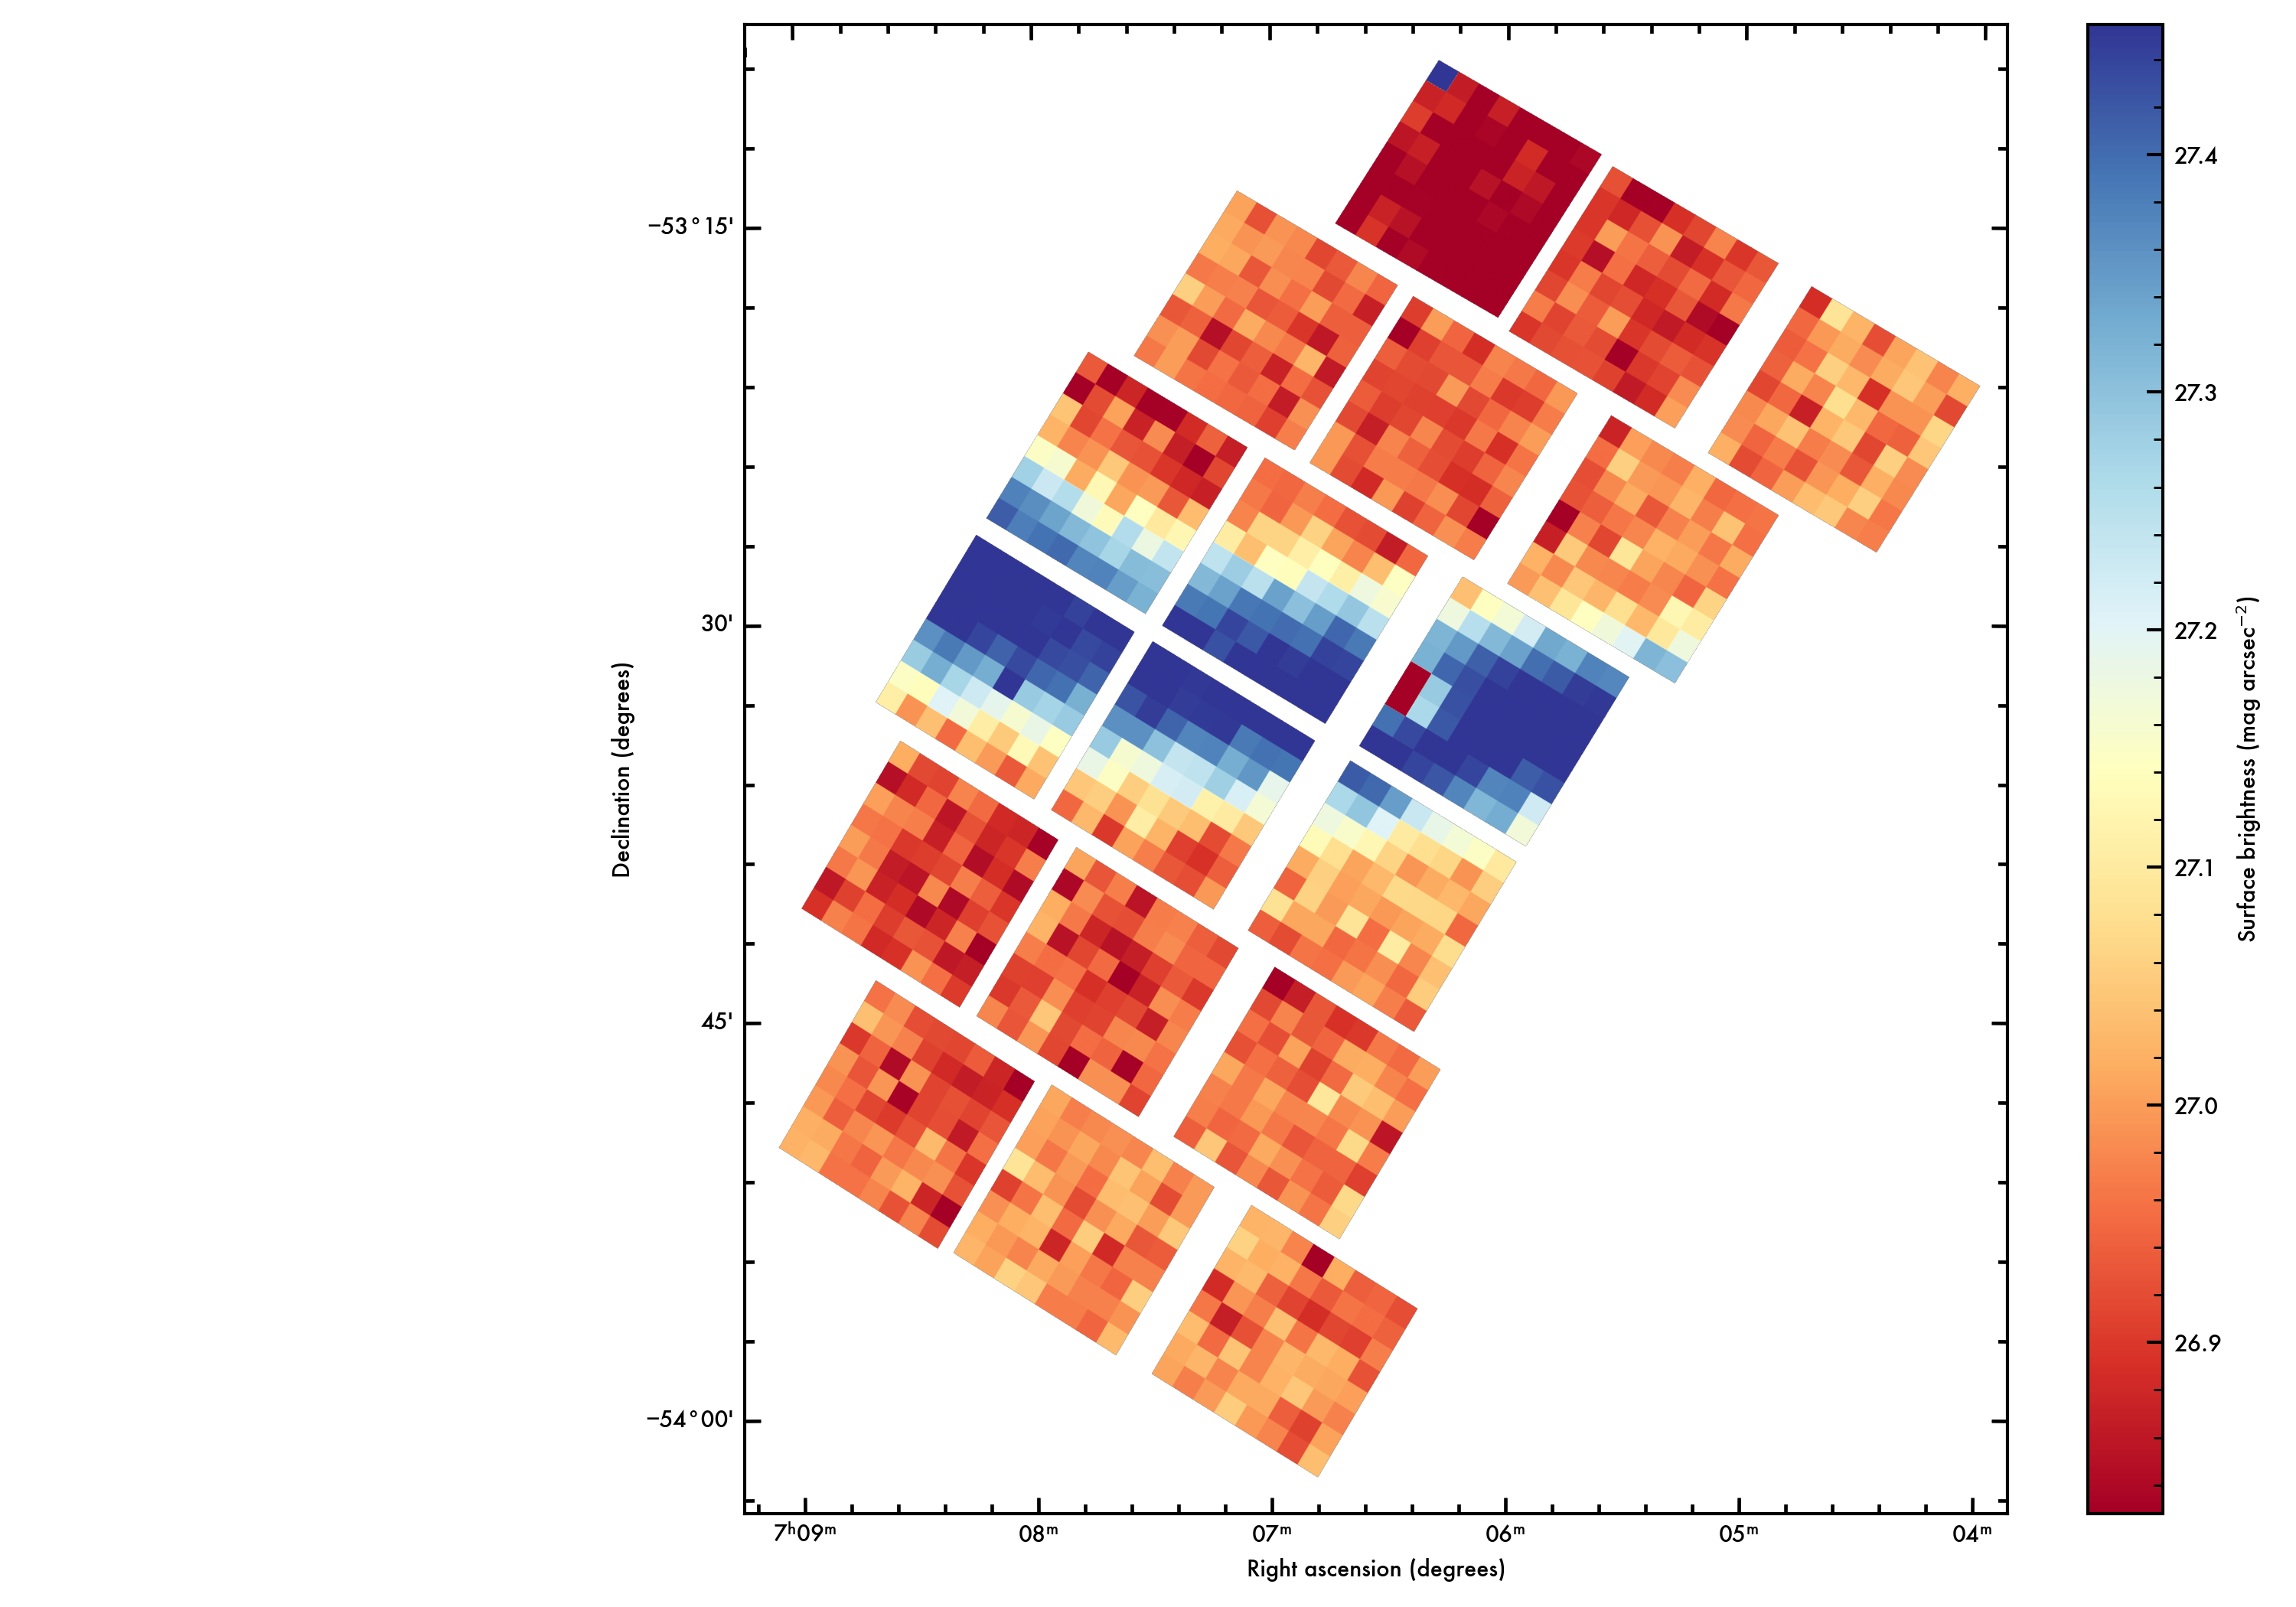
\includegraphics[trim={180 0 10 0}, clip, width=0.475\textwidth]{WFI_F129_RA_106.624_DEC_-53.595_MJD_61365.00000_PA_-121.23_stray_drz_scaled_fe2mu.png}
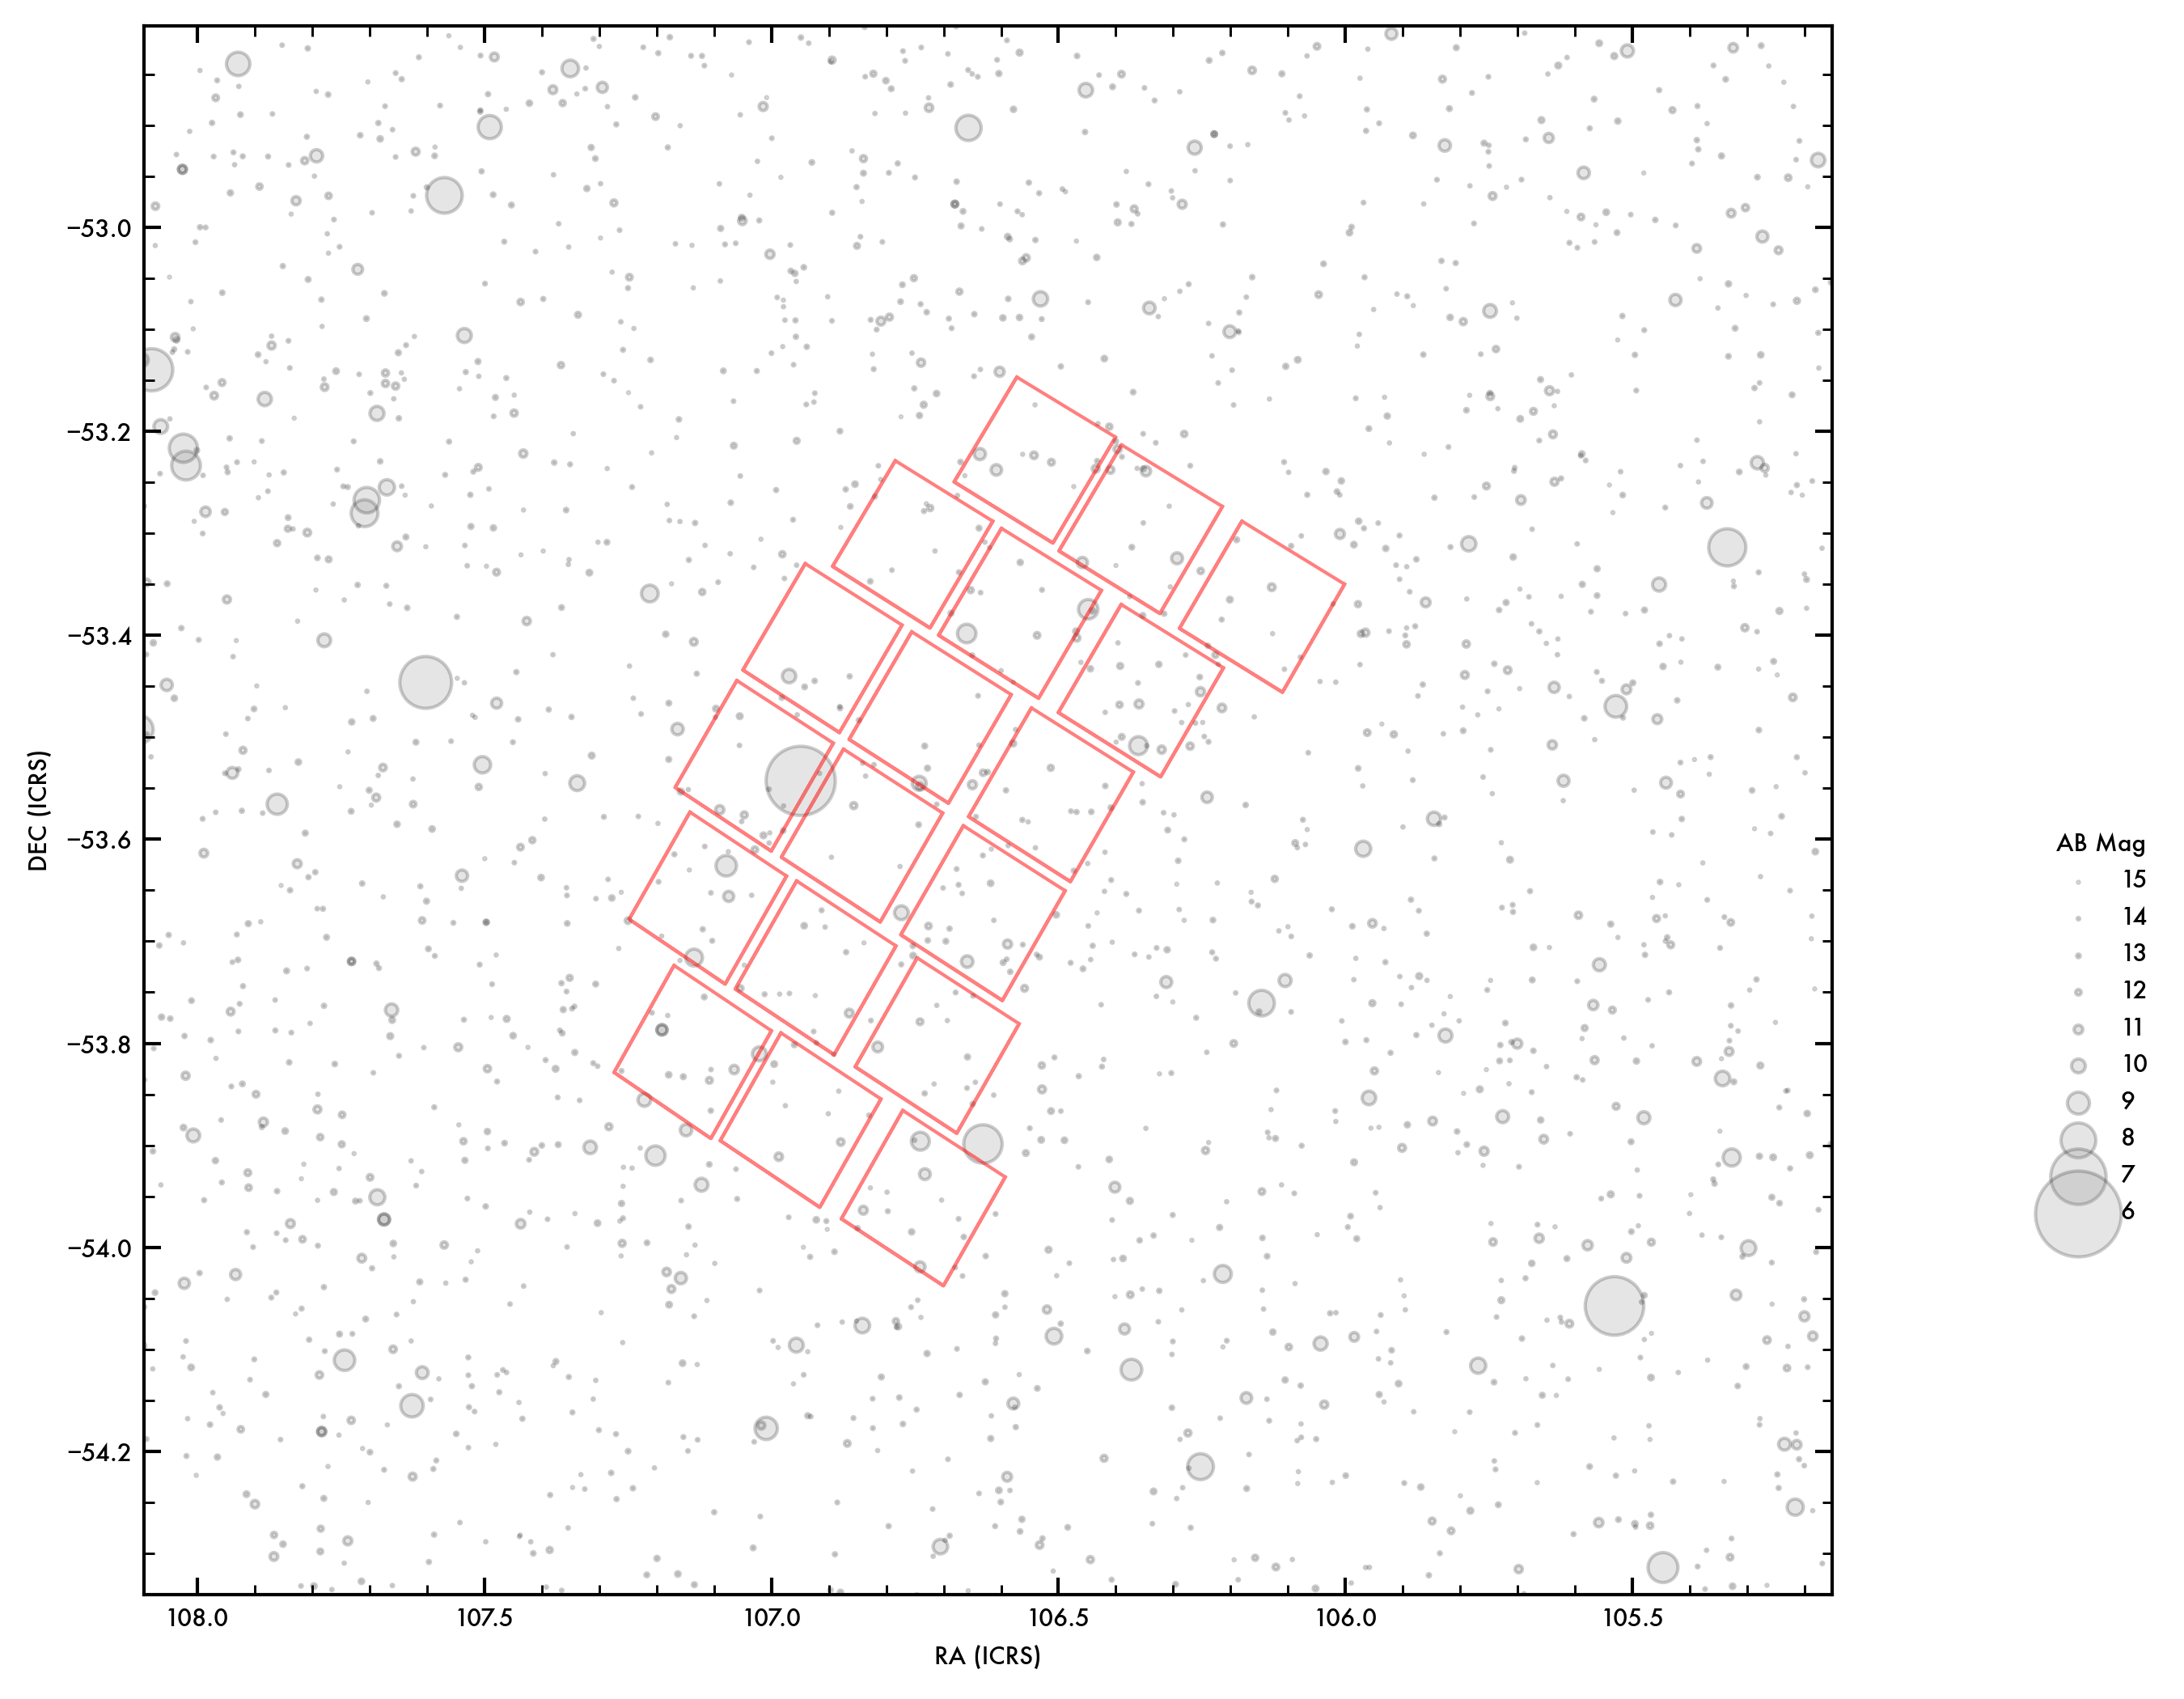
\includegraphics[trim={0 0 80 0}, clip, width=0.515\textwidth]{WFI_F129_RA_106.624_DEC_-53.595_MJD_61365.00000_PA_-121.23_stars_close.png}
\caption{Normalized Detector Irradiance for \emph{Nancy Grace Roman} Space Telescope Wide Field Instrument (WFI), showing the regions of maximum stray-light sensitivity. \emph{Left:} Detail around $2\times2$ degrees from the center of the WFI focal plane. \emph{Right:} NDI map at $20\times20$ degrees from WFI.} 
\label{fig:Secondary_leg}
\end{center}
\end{figure*}




\subsection{High Latitude Wide Area Survey}\label{subsec:HLWAS}

The preliminary coordinates for the observations of the HWLAS are presented in Fig.\,\ref{fig:HWLAS}\footnote{\url{https://www.stsci.edu/files/live/sites/www/files/home/roman/_documents/Roman-STScI-000457-SOC-PSS.pdf}}. The exact coordinates and roll angles of each exposure will depend on the exact observation epoch, but we can assume the representative set of targets as described in the \emph{Roman}/WFI will be positioned with the best roll angle against the Sun orientation. For this example, we assume June 2027 as the observation epoch.\\

The predicted gradients for those observations are shown in Fig.\,\ref{fig:HWLAS_examples}. The intensity of the stray-light background levels extends between $\mu = 28.5$ to 29.0 \magarc, with an average on $\mu = 28.7$ \magarc. These results are 3 magnitudes lower than the predicted pre-launch stray-light background levels for \emph{Euclid}/VIS. The results show characteristic patterns that repeat across all exposures, like a higher sensitivity to stray-light on SCA18 or cases of Dragon's Breath under the first row of detectors. These patterns will allow us to understand and predict better all types of systematic backgrounds to improve low surface brightness imaging with \emph{Roman}/WFI.


\begin{figure*}[hbt!]
 \begin{center}
 % trim left bottom right top 
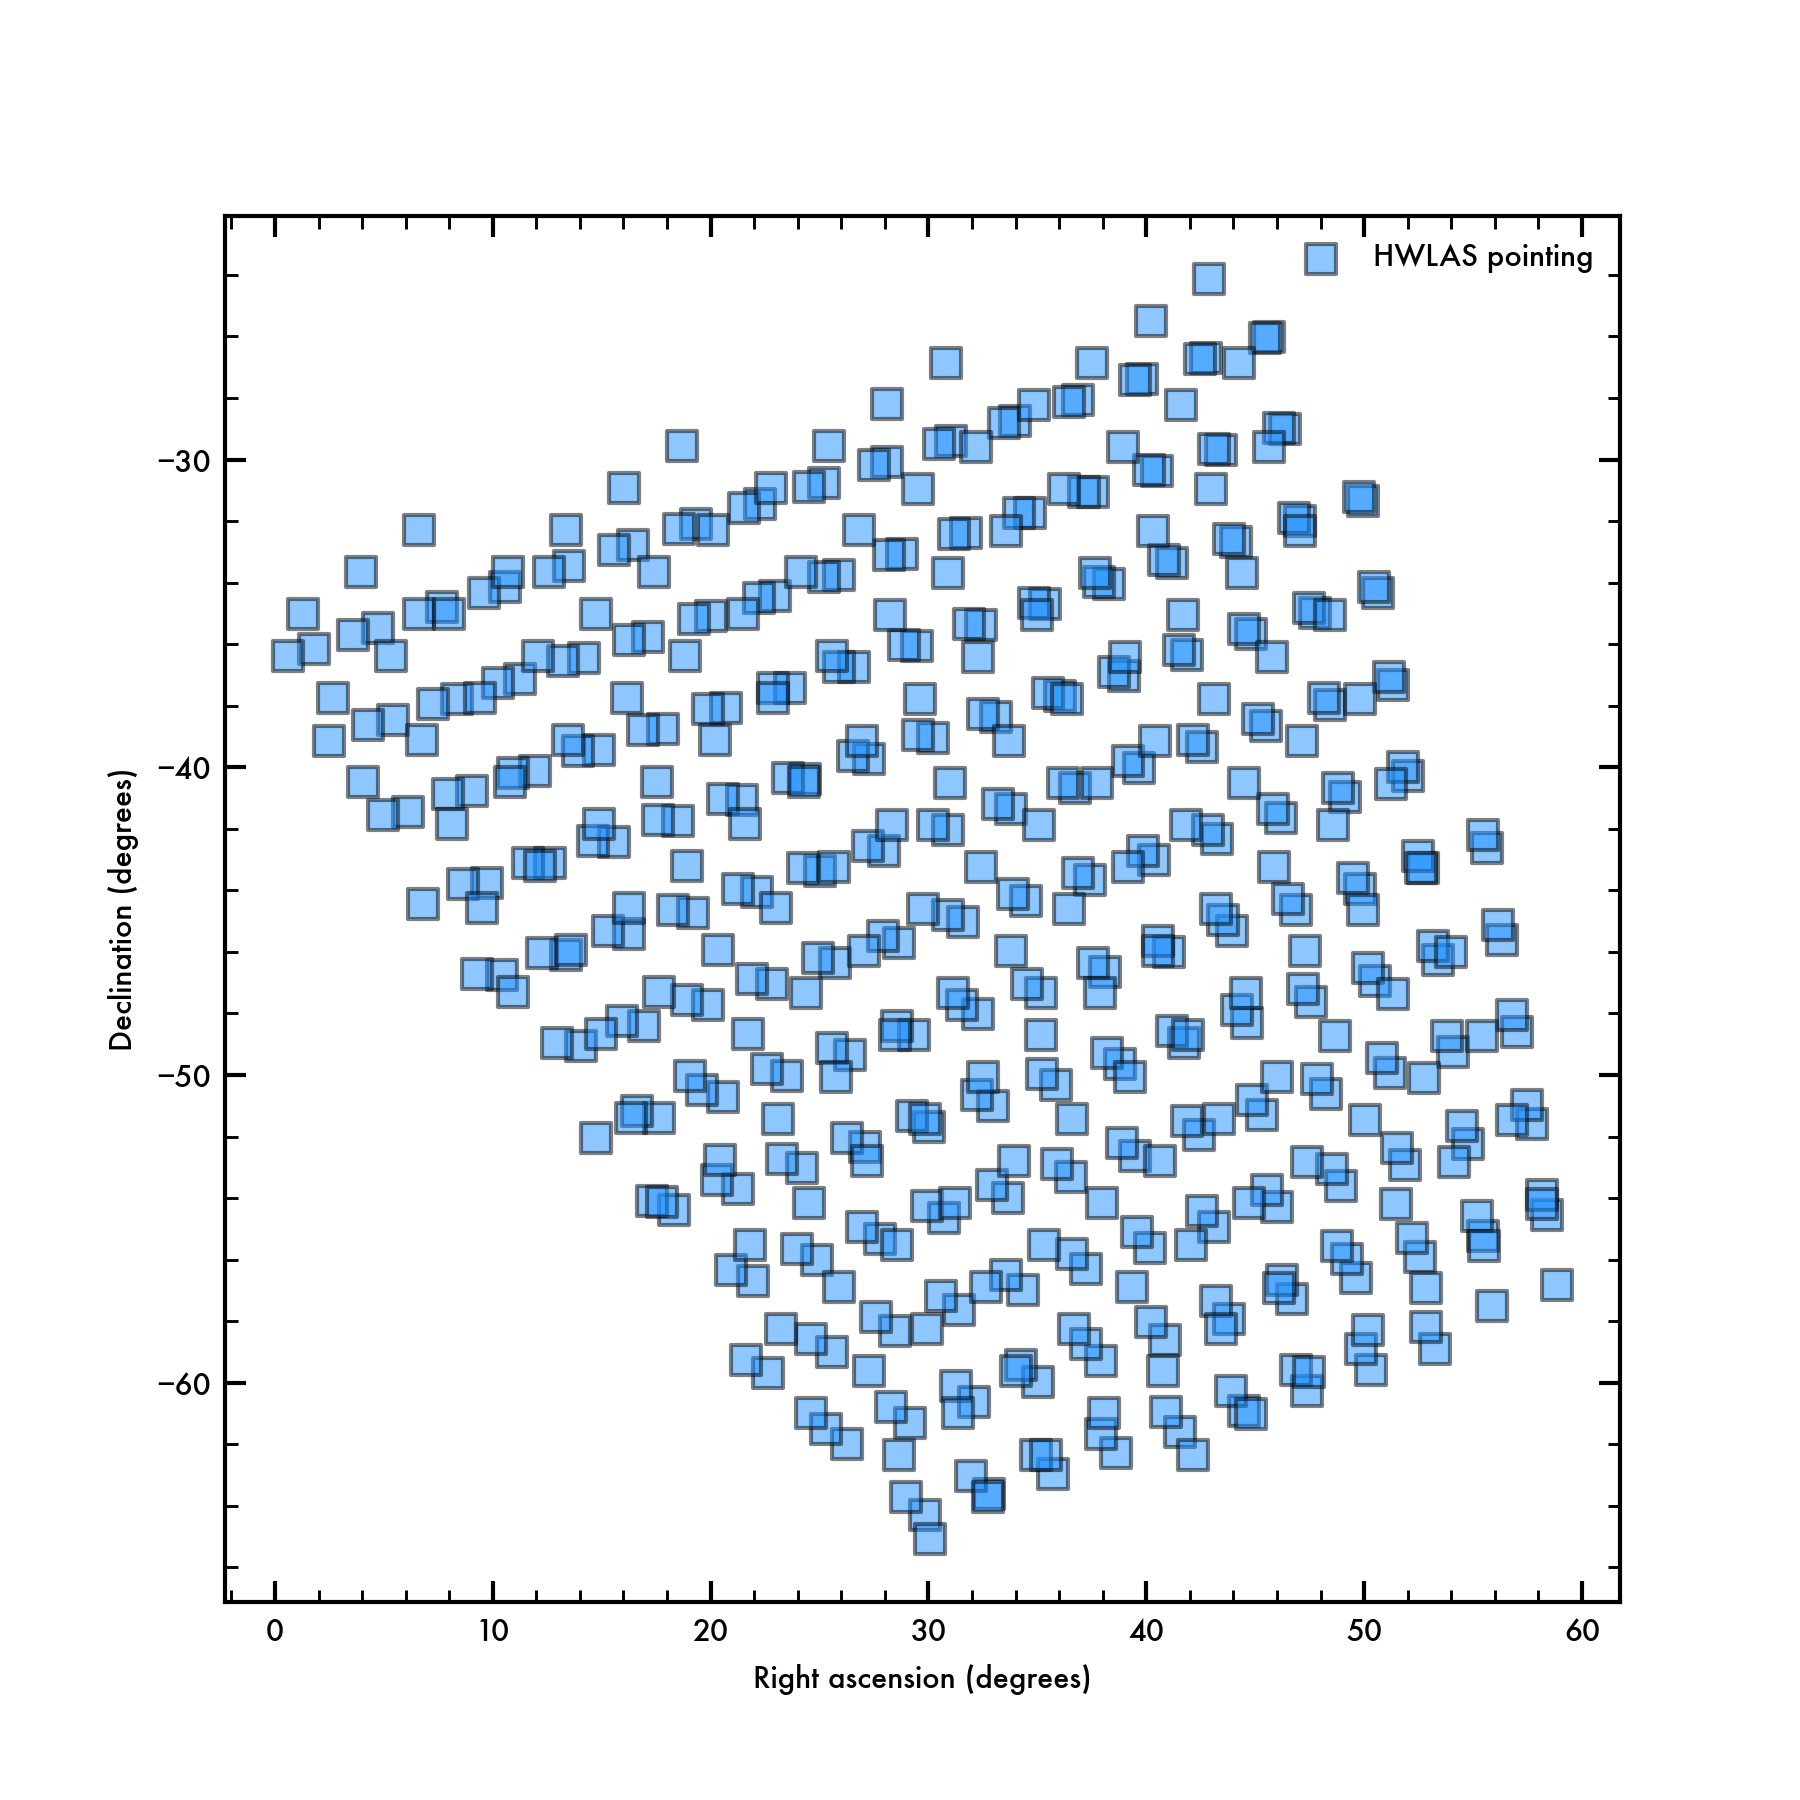
\includegraphics[trim={0 0 0 0}, clip, width=0.435\textwidth]{HWLAS_coords.png}
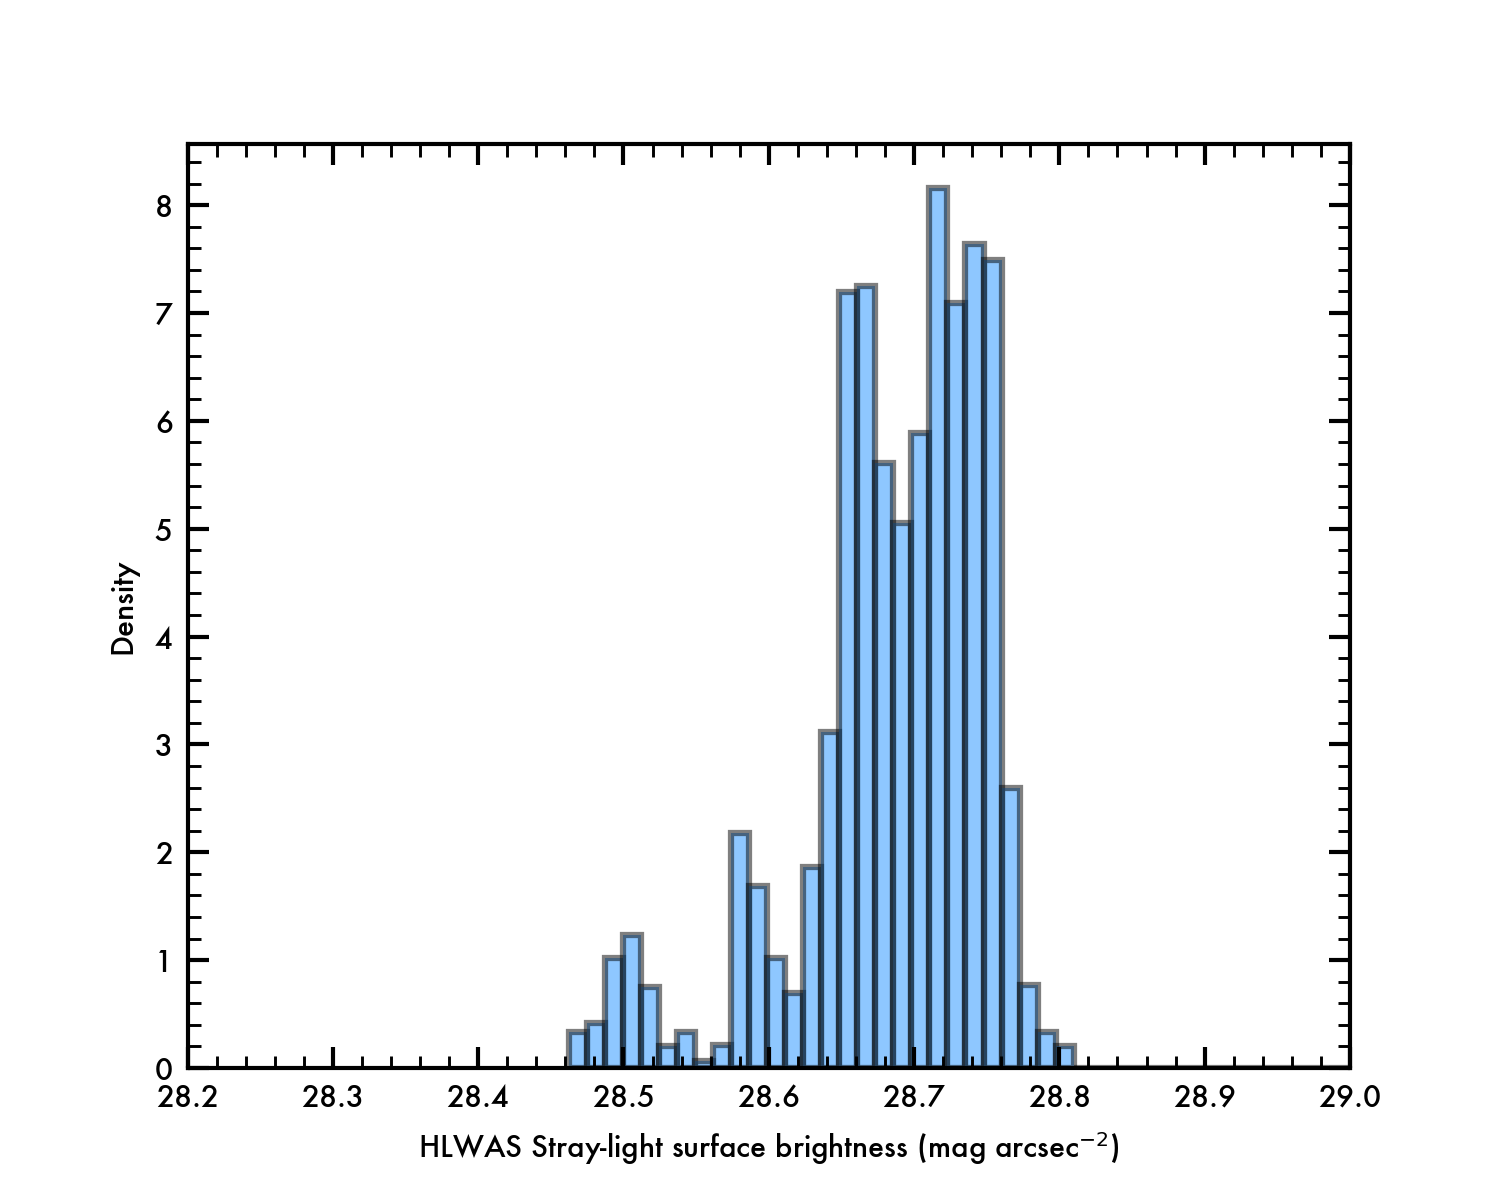
\includegraphics[trim={0 0 0 0}, clip, width=0.555\textwidth]{HWLAS_straylight_hist.png}
\caption{\emph{Left panel}: Approximate footprint for a section of the High Latitude Wide Area Survey (HWLAS \emph{Roman} PID 991 . \emph{Right panel}: Stray-light background surface brightness magnitude for the simulated frames. Notice the expected low intensity ranged between  $\mu = 28.5$ to 29.0 \magarc.} 
\label{fig:HWLAS}
\end{center}
\end{figure*}


\begin{figure*}[hbt!]
 \begin{center}
 % trim left bottom right top 
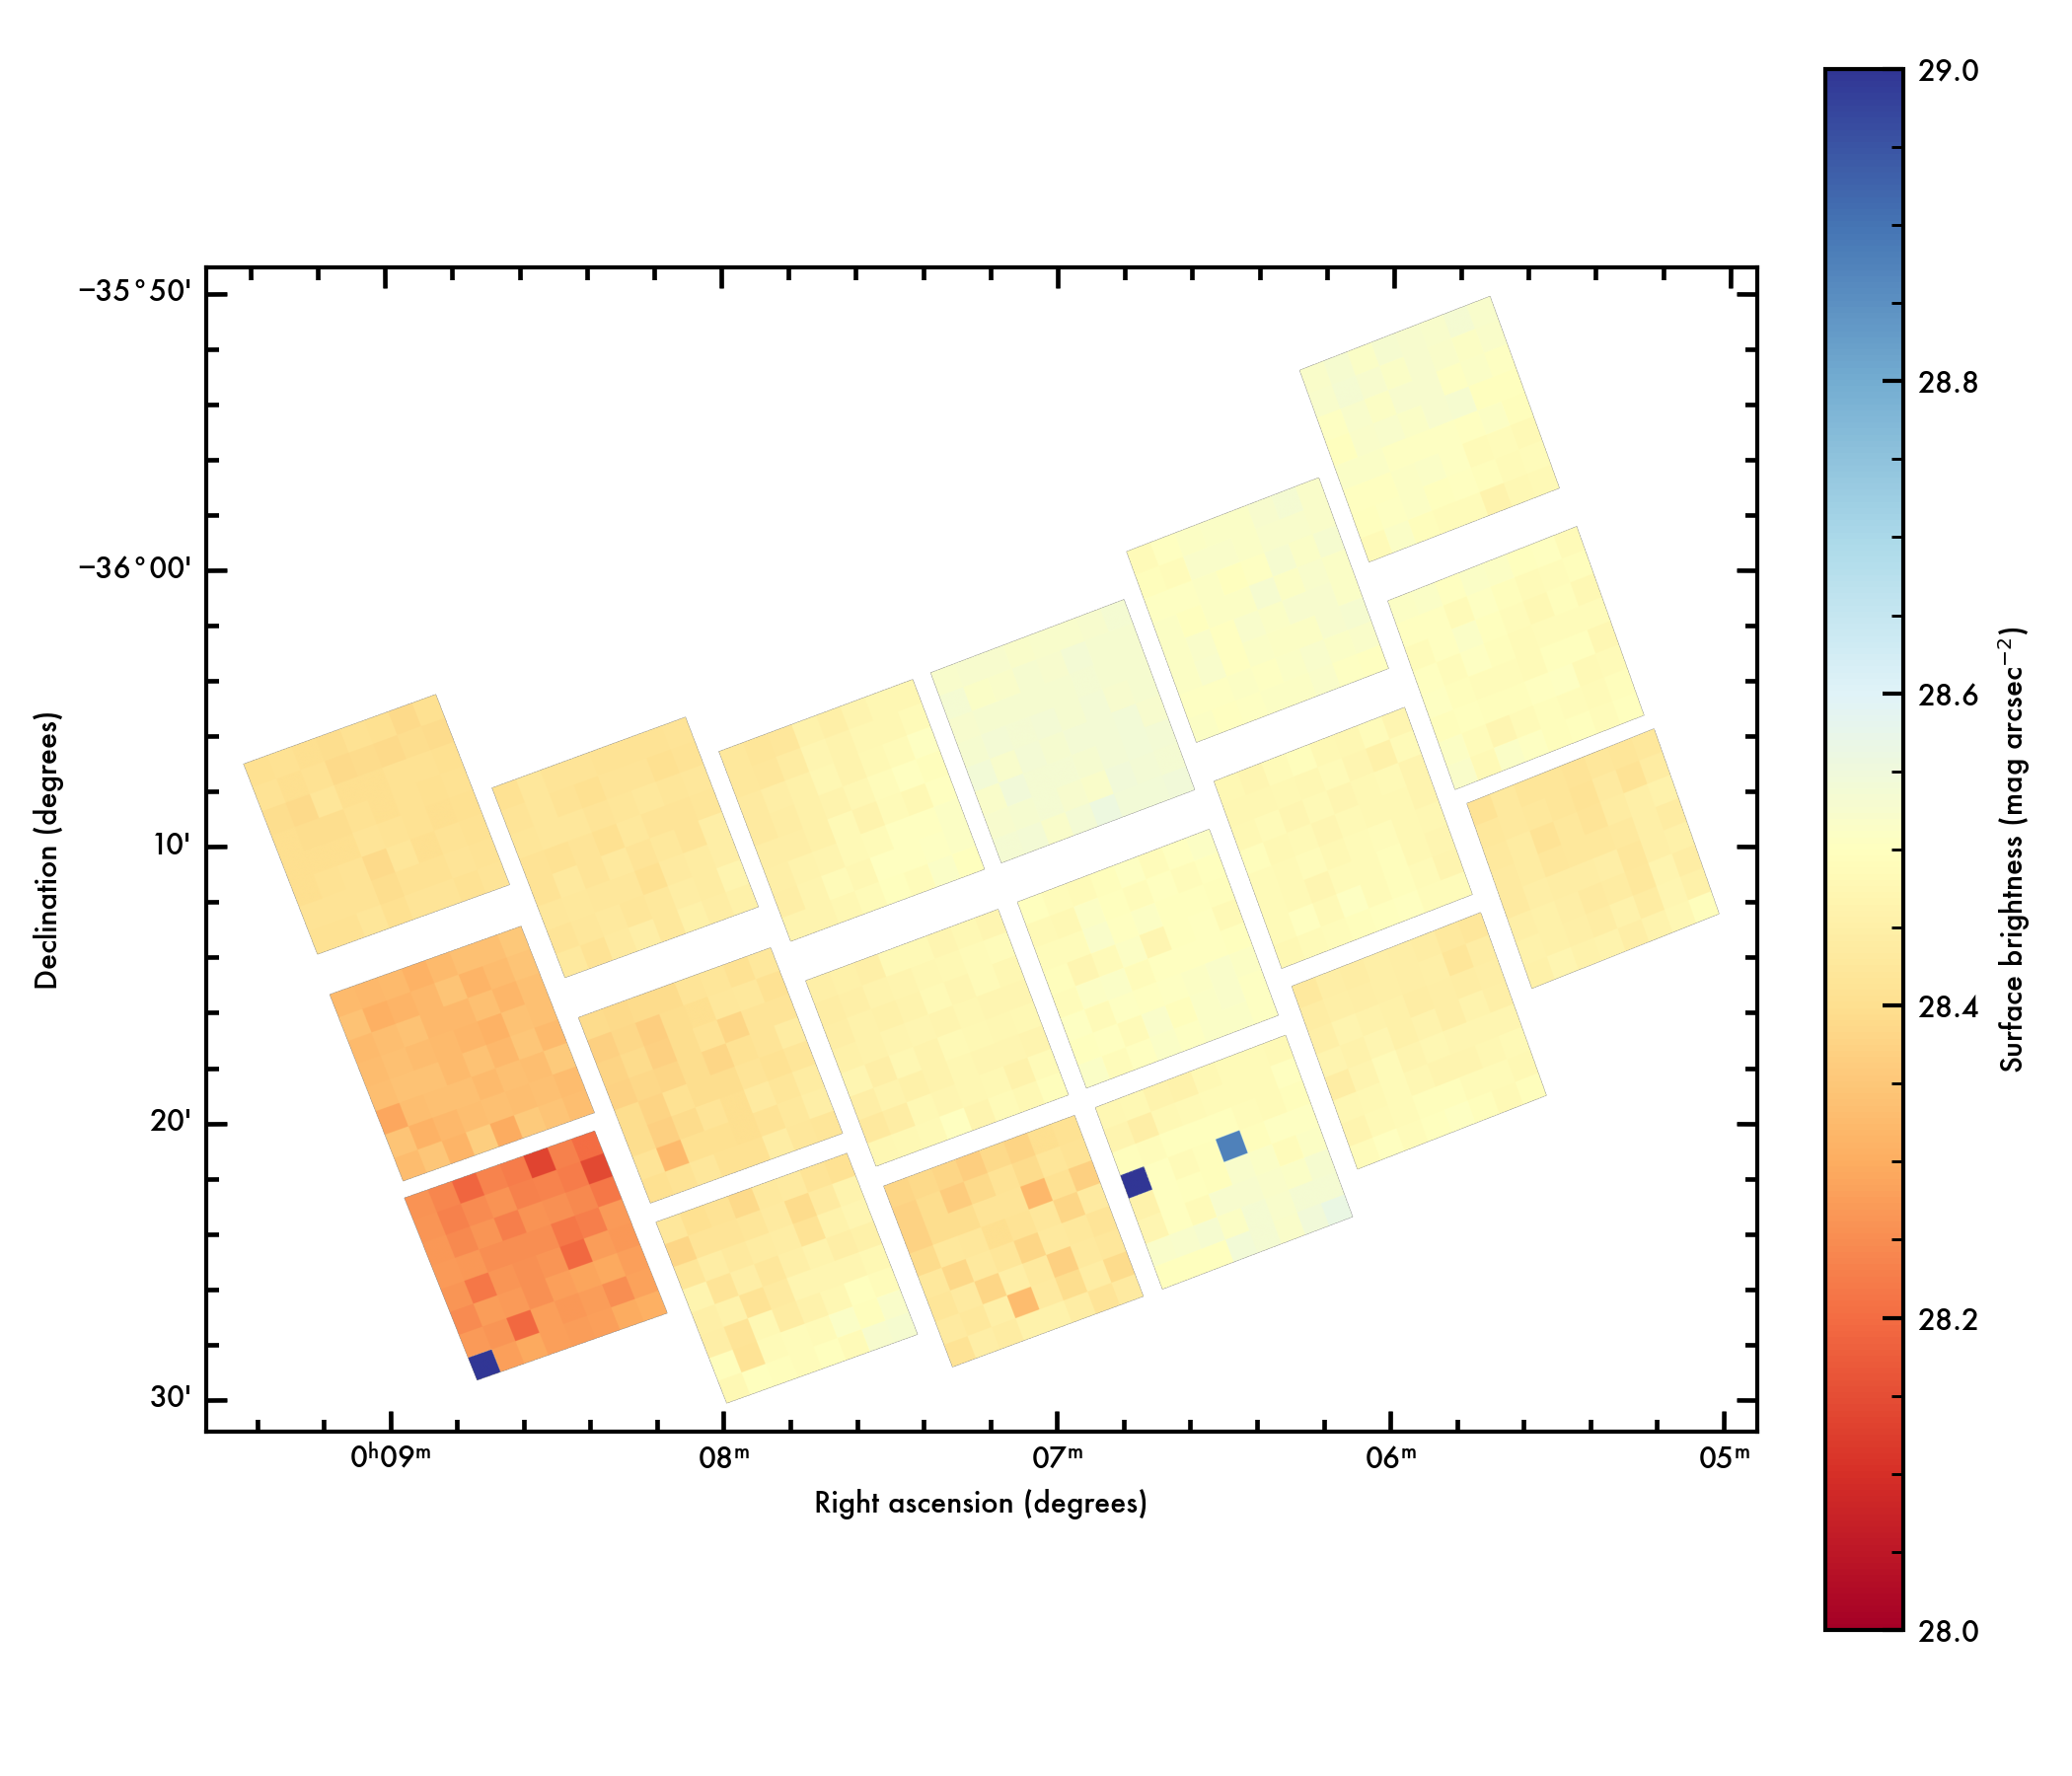
\includegraphics[trim={0 0 0 0}, clip, width=0.495\textwidth]{HWLAS77_WFI_F129_RA_001.810_DEC_-36.156_MJD_61577.00000_PA_020.57_stray_drz_scaled_fe2mu.png}
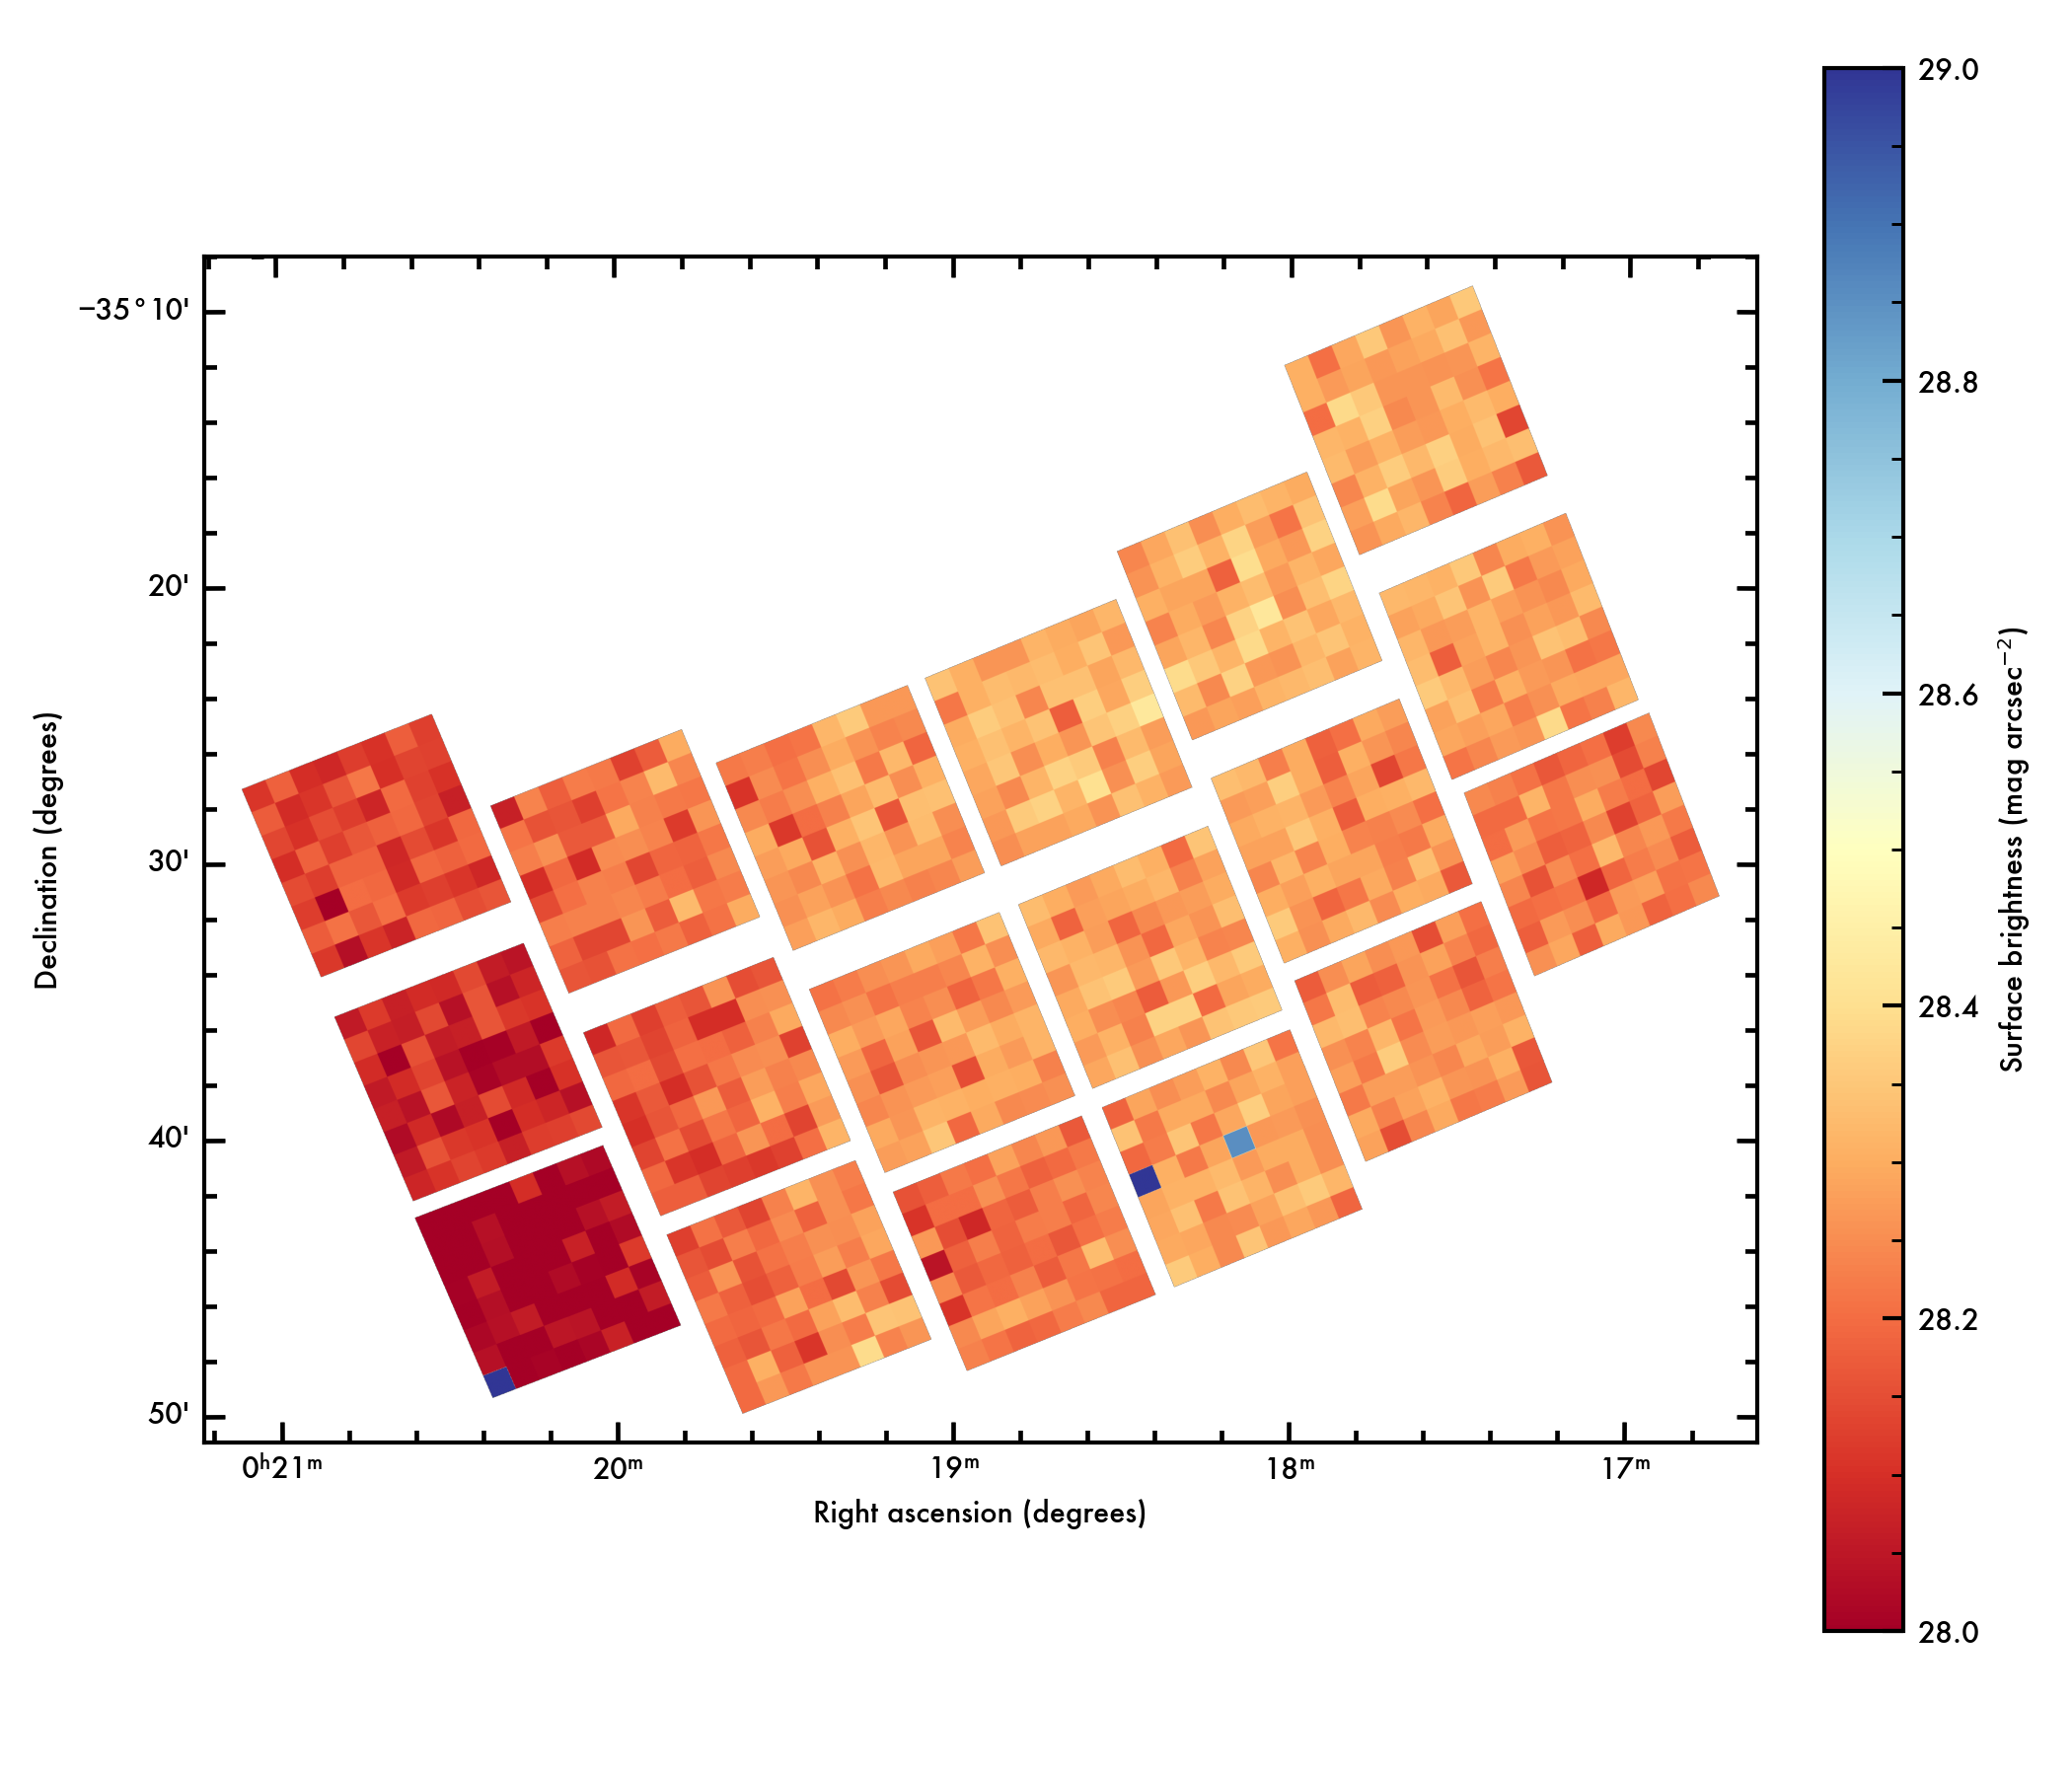
\includegraphics[trim={0 0 0 0}, clip, width=0.495\textwidth]{HWLAS77_WFI_F129_RA_004.733_DEC_-35.481_MJD_61577.00000_PA_022.24_stray_drz_scaled_fe2mu.png}

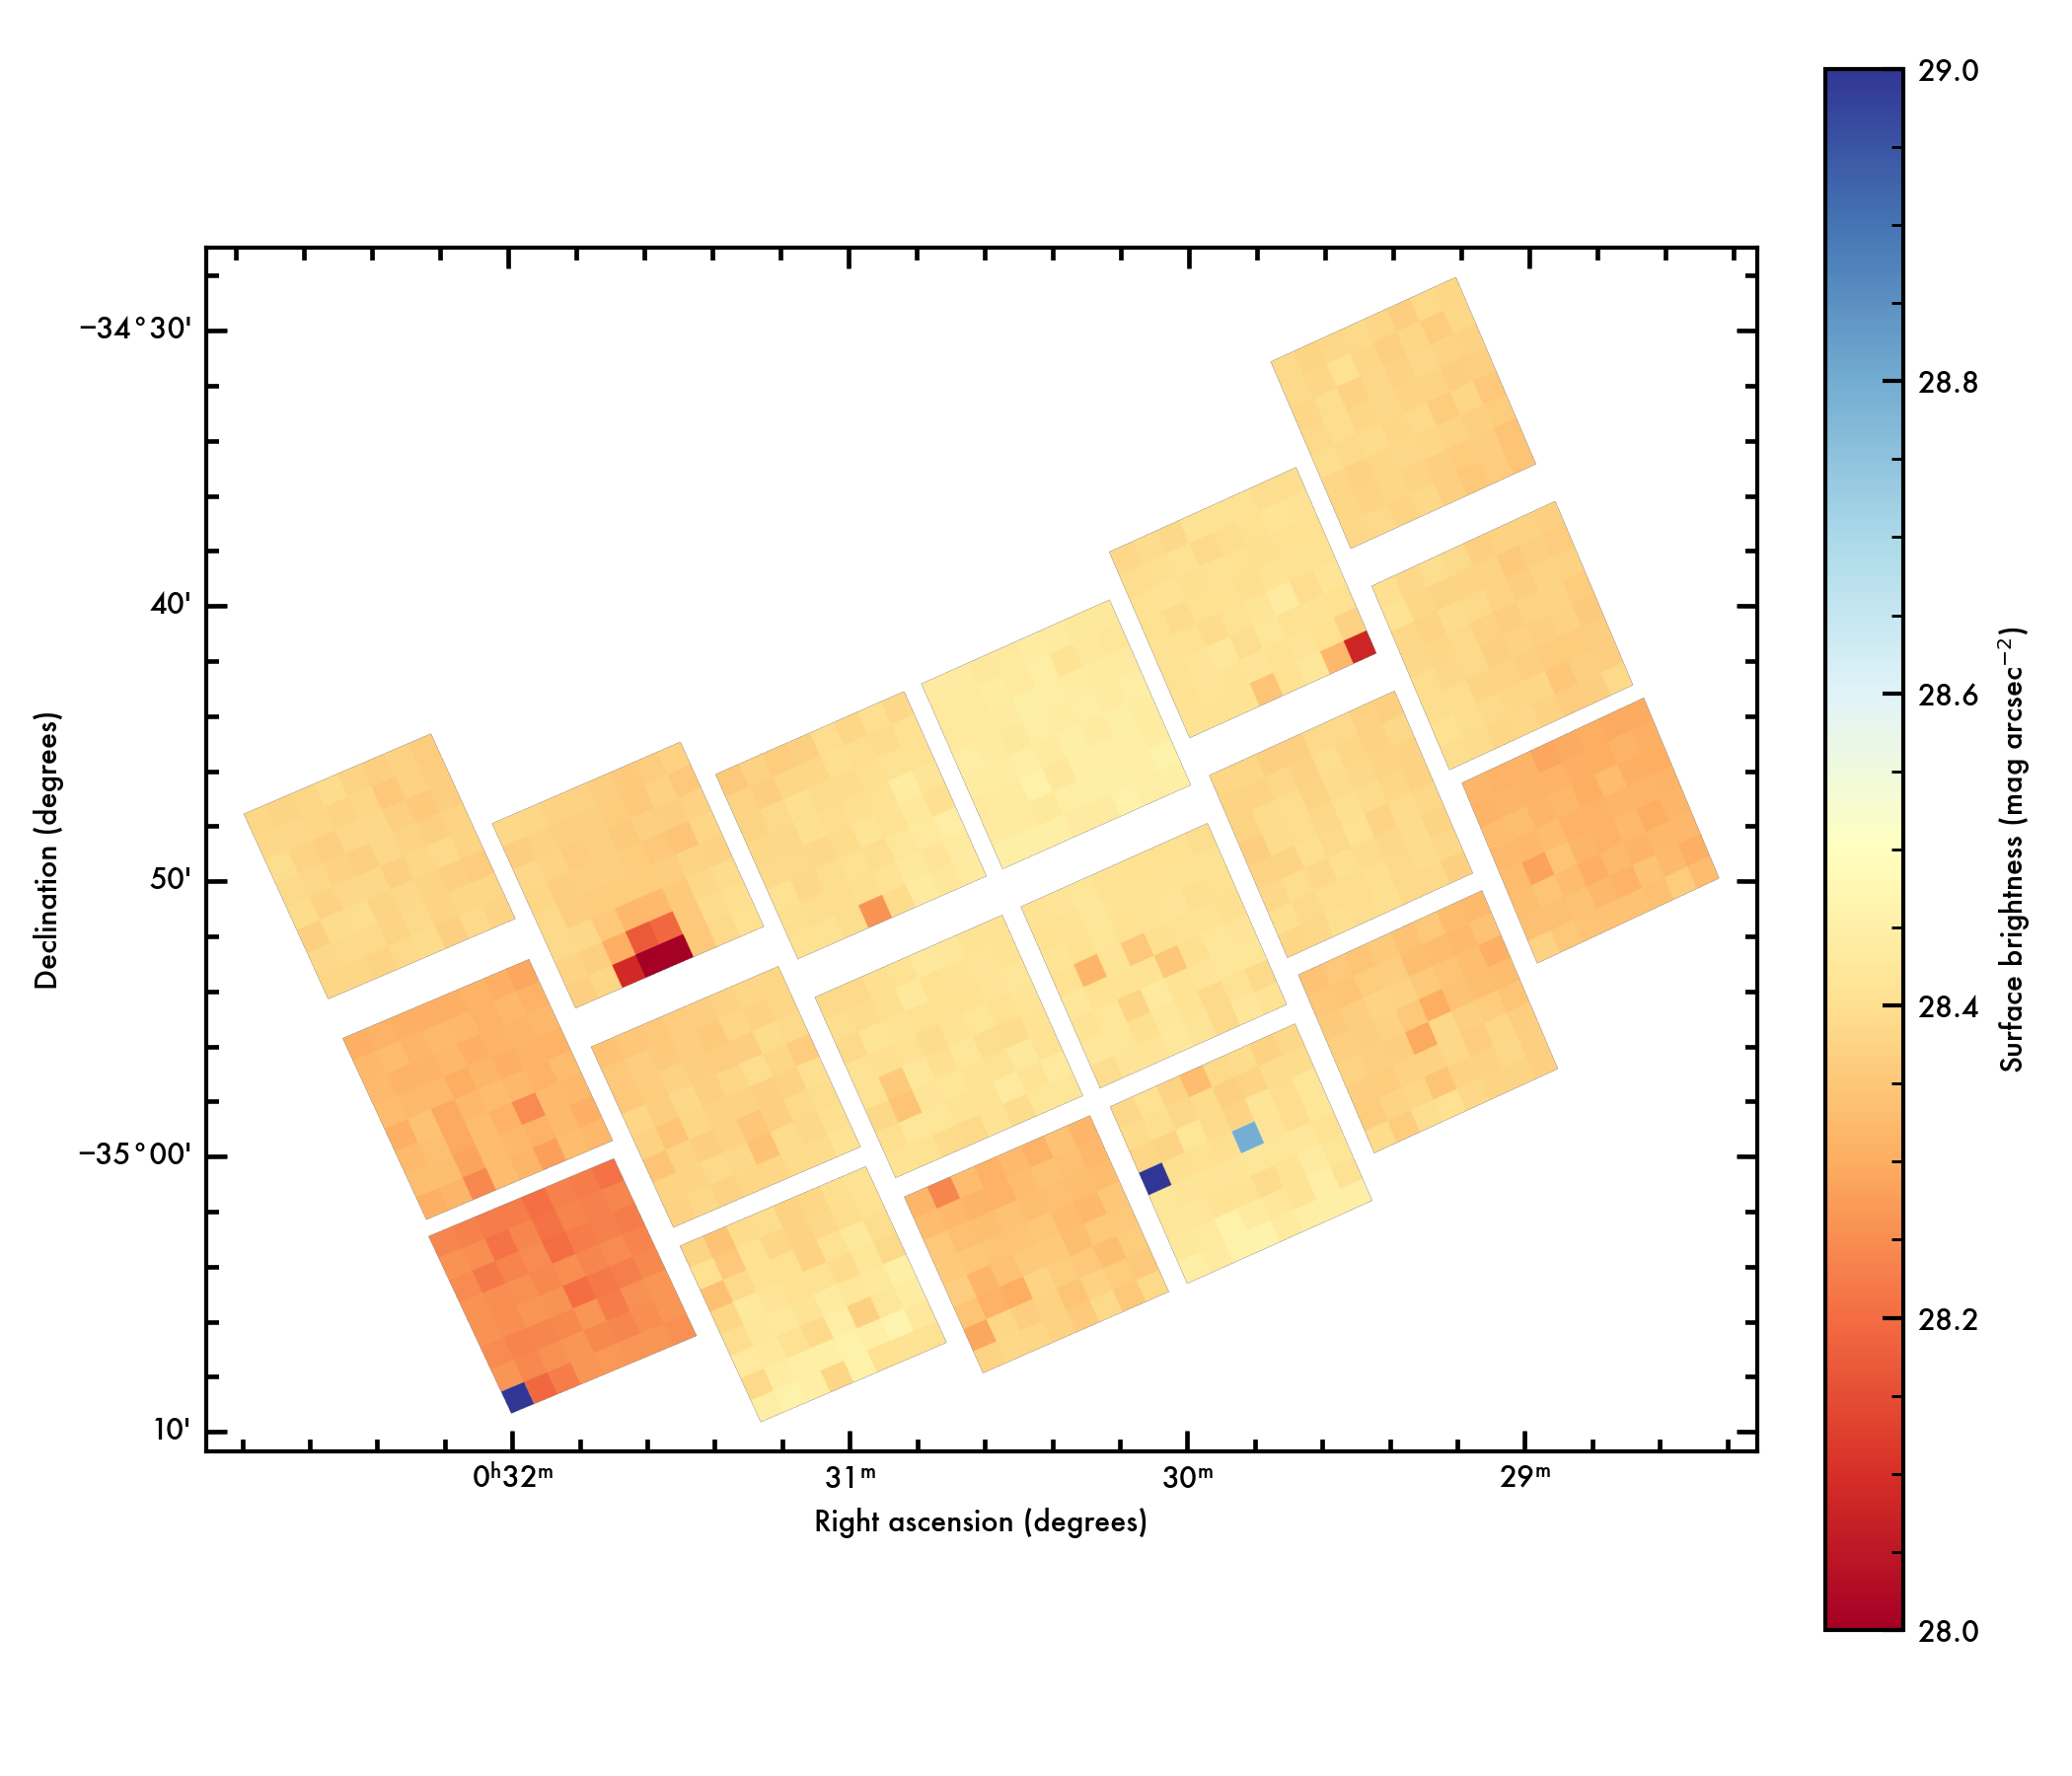
\includegraphics[trim={0 0 0 0}, clip, width=0.495\textwidth]{HWLAS77_WFI_F129_RA_007.656_DEC_-34.806_MJD_61577.00000_PA_023.88_stray_drz_scaled_fe2mu.png}
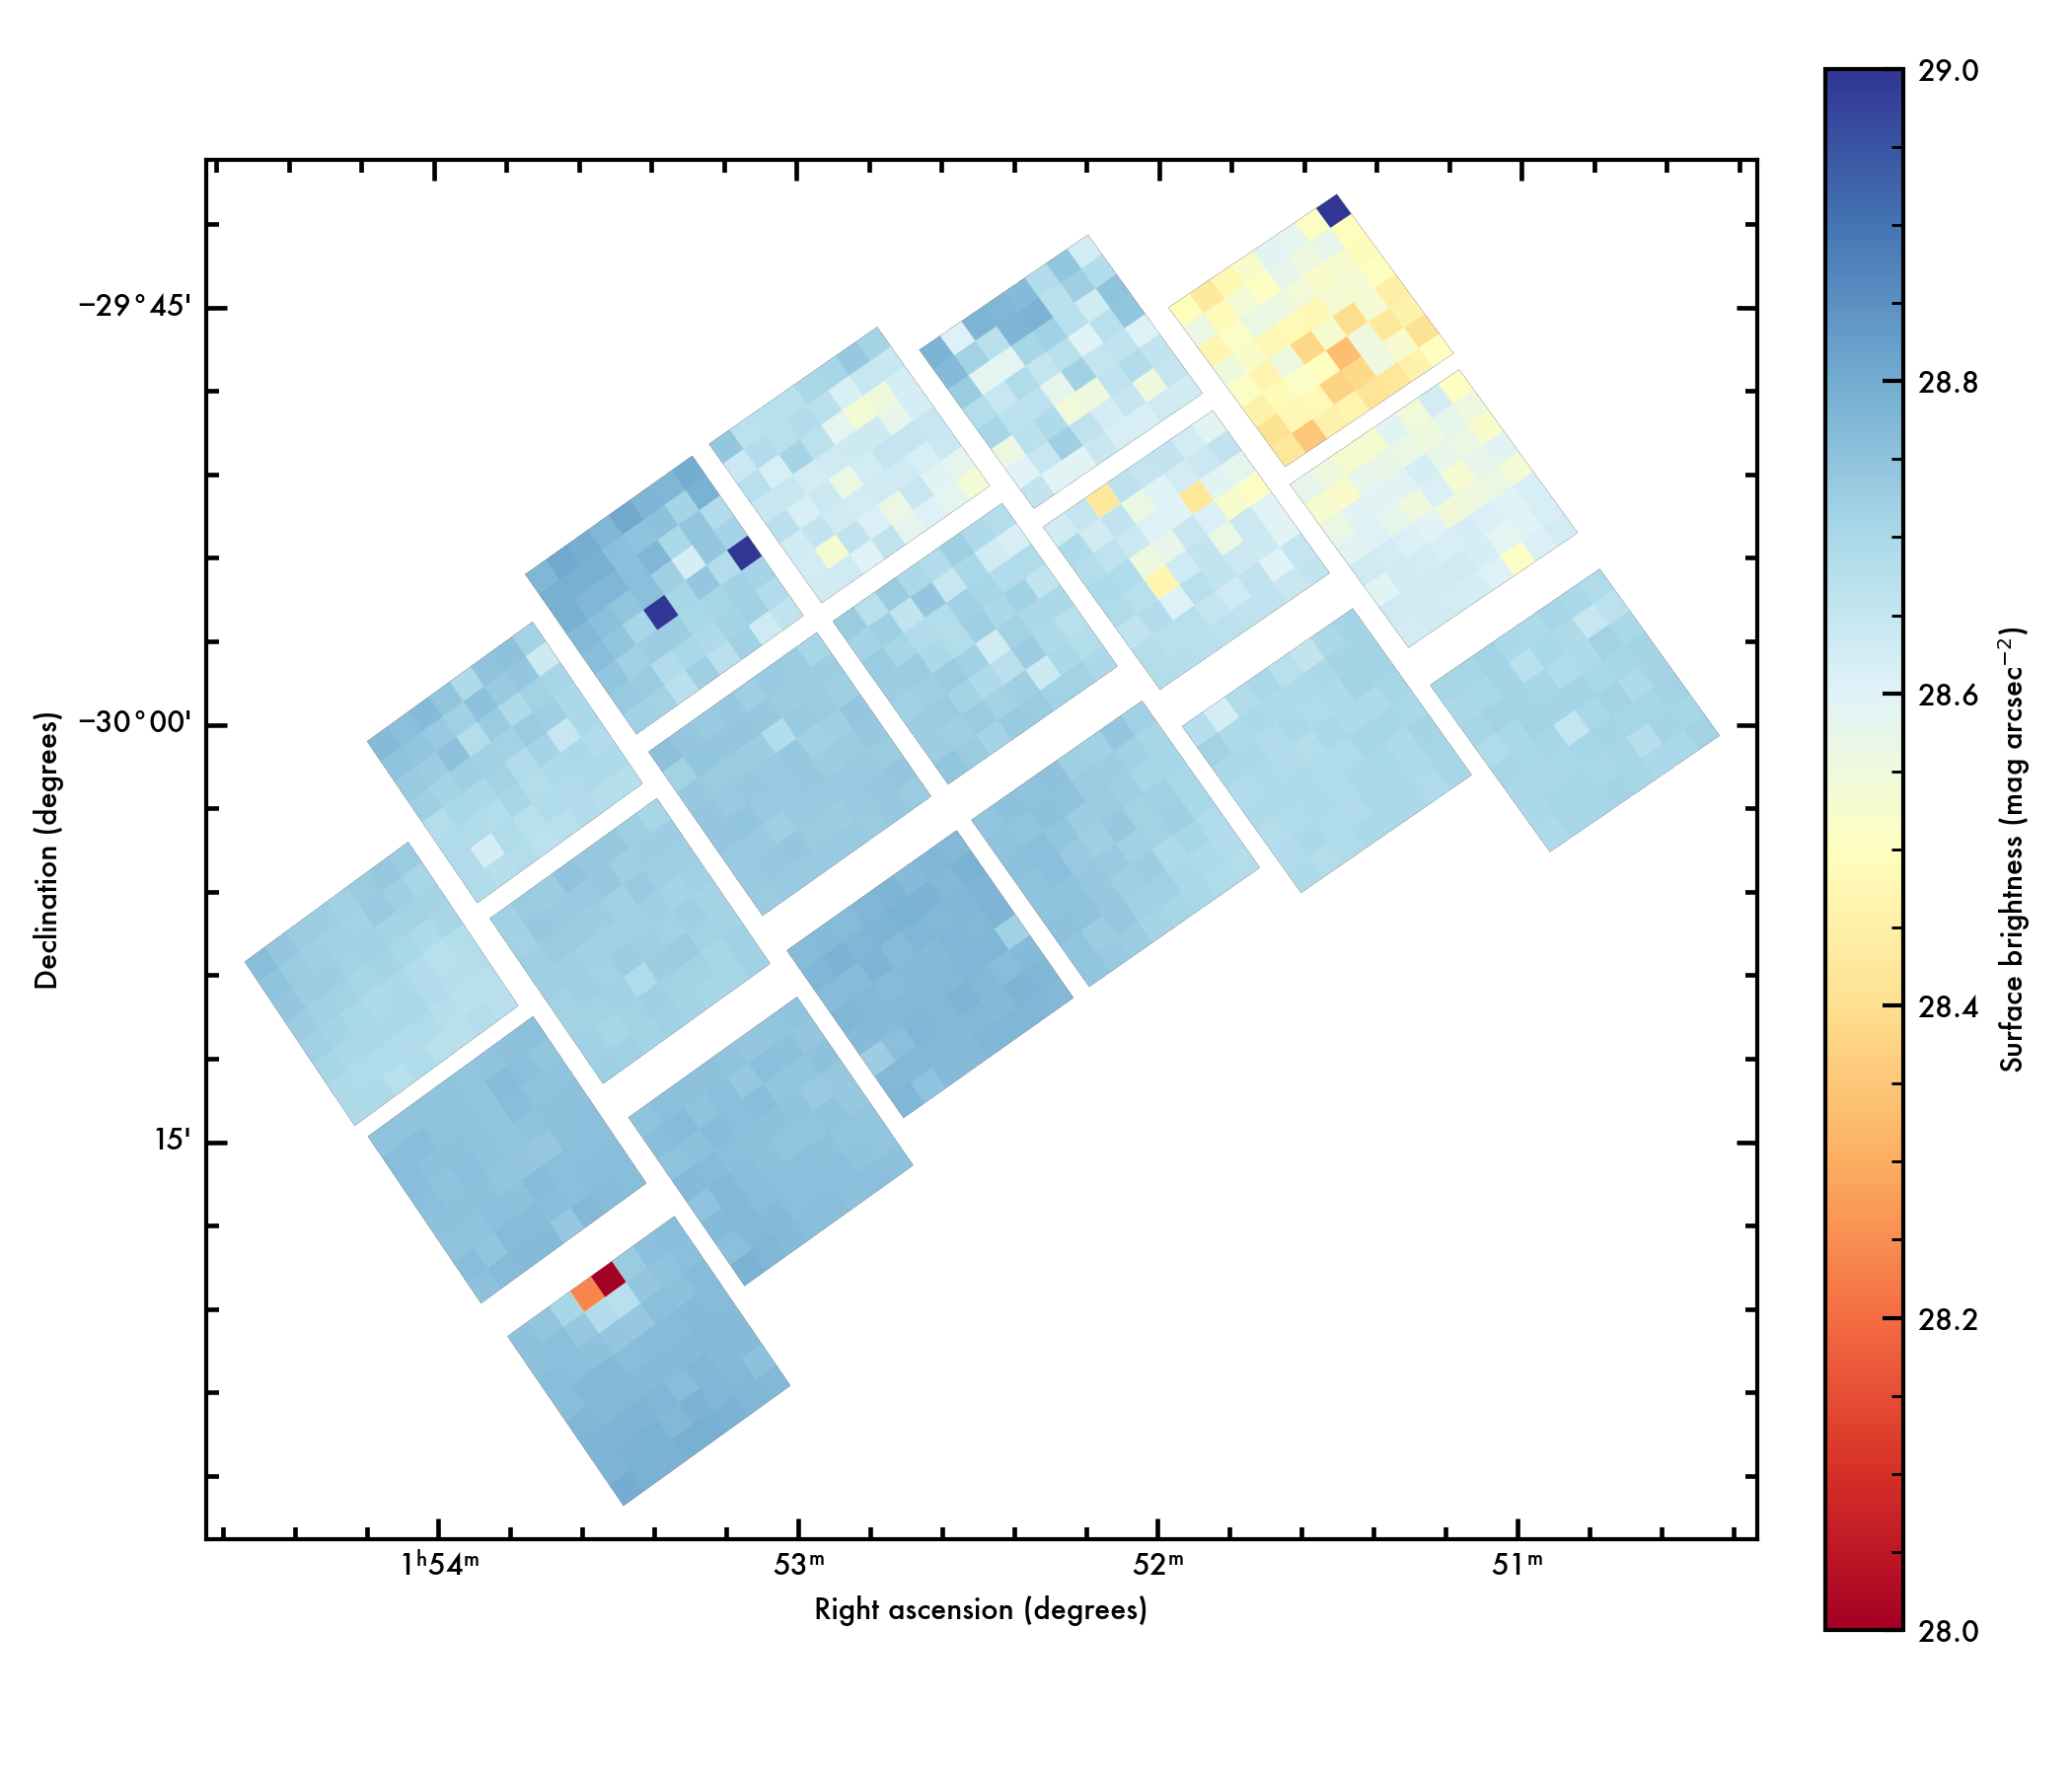
\includegraphics[trim={0 0 0 0}, clip, width=0.495\textwidth]{HWLAS77_WFI_F129_RA_028.118_DEC_-30.082_MJD_61577.00000_PA_-144.91_stray_drz_scaled_fe2mu.png}

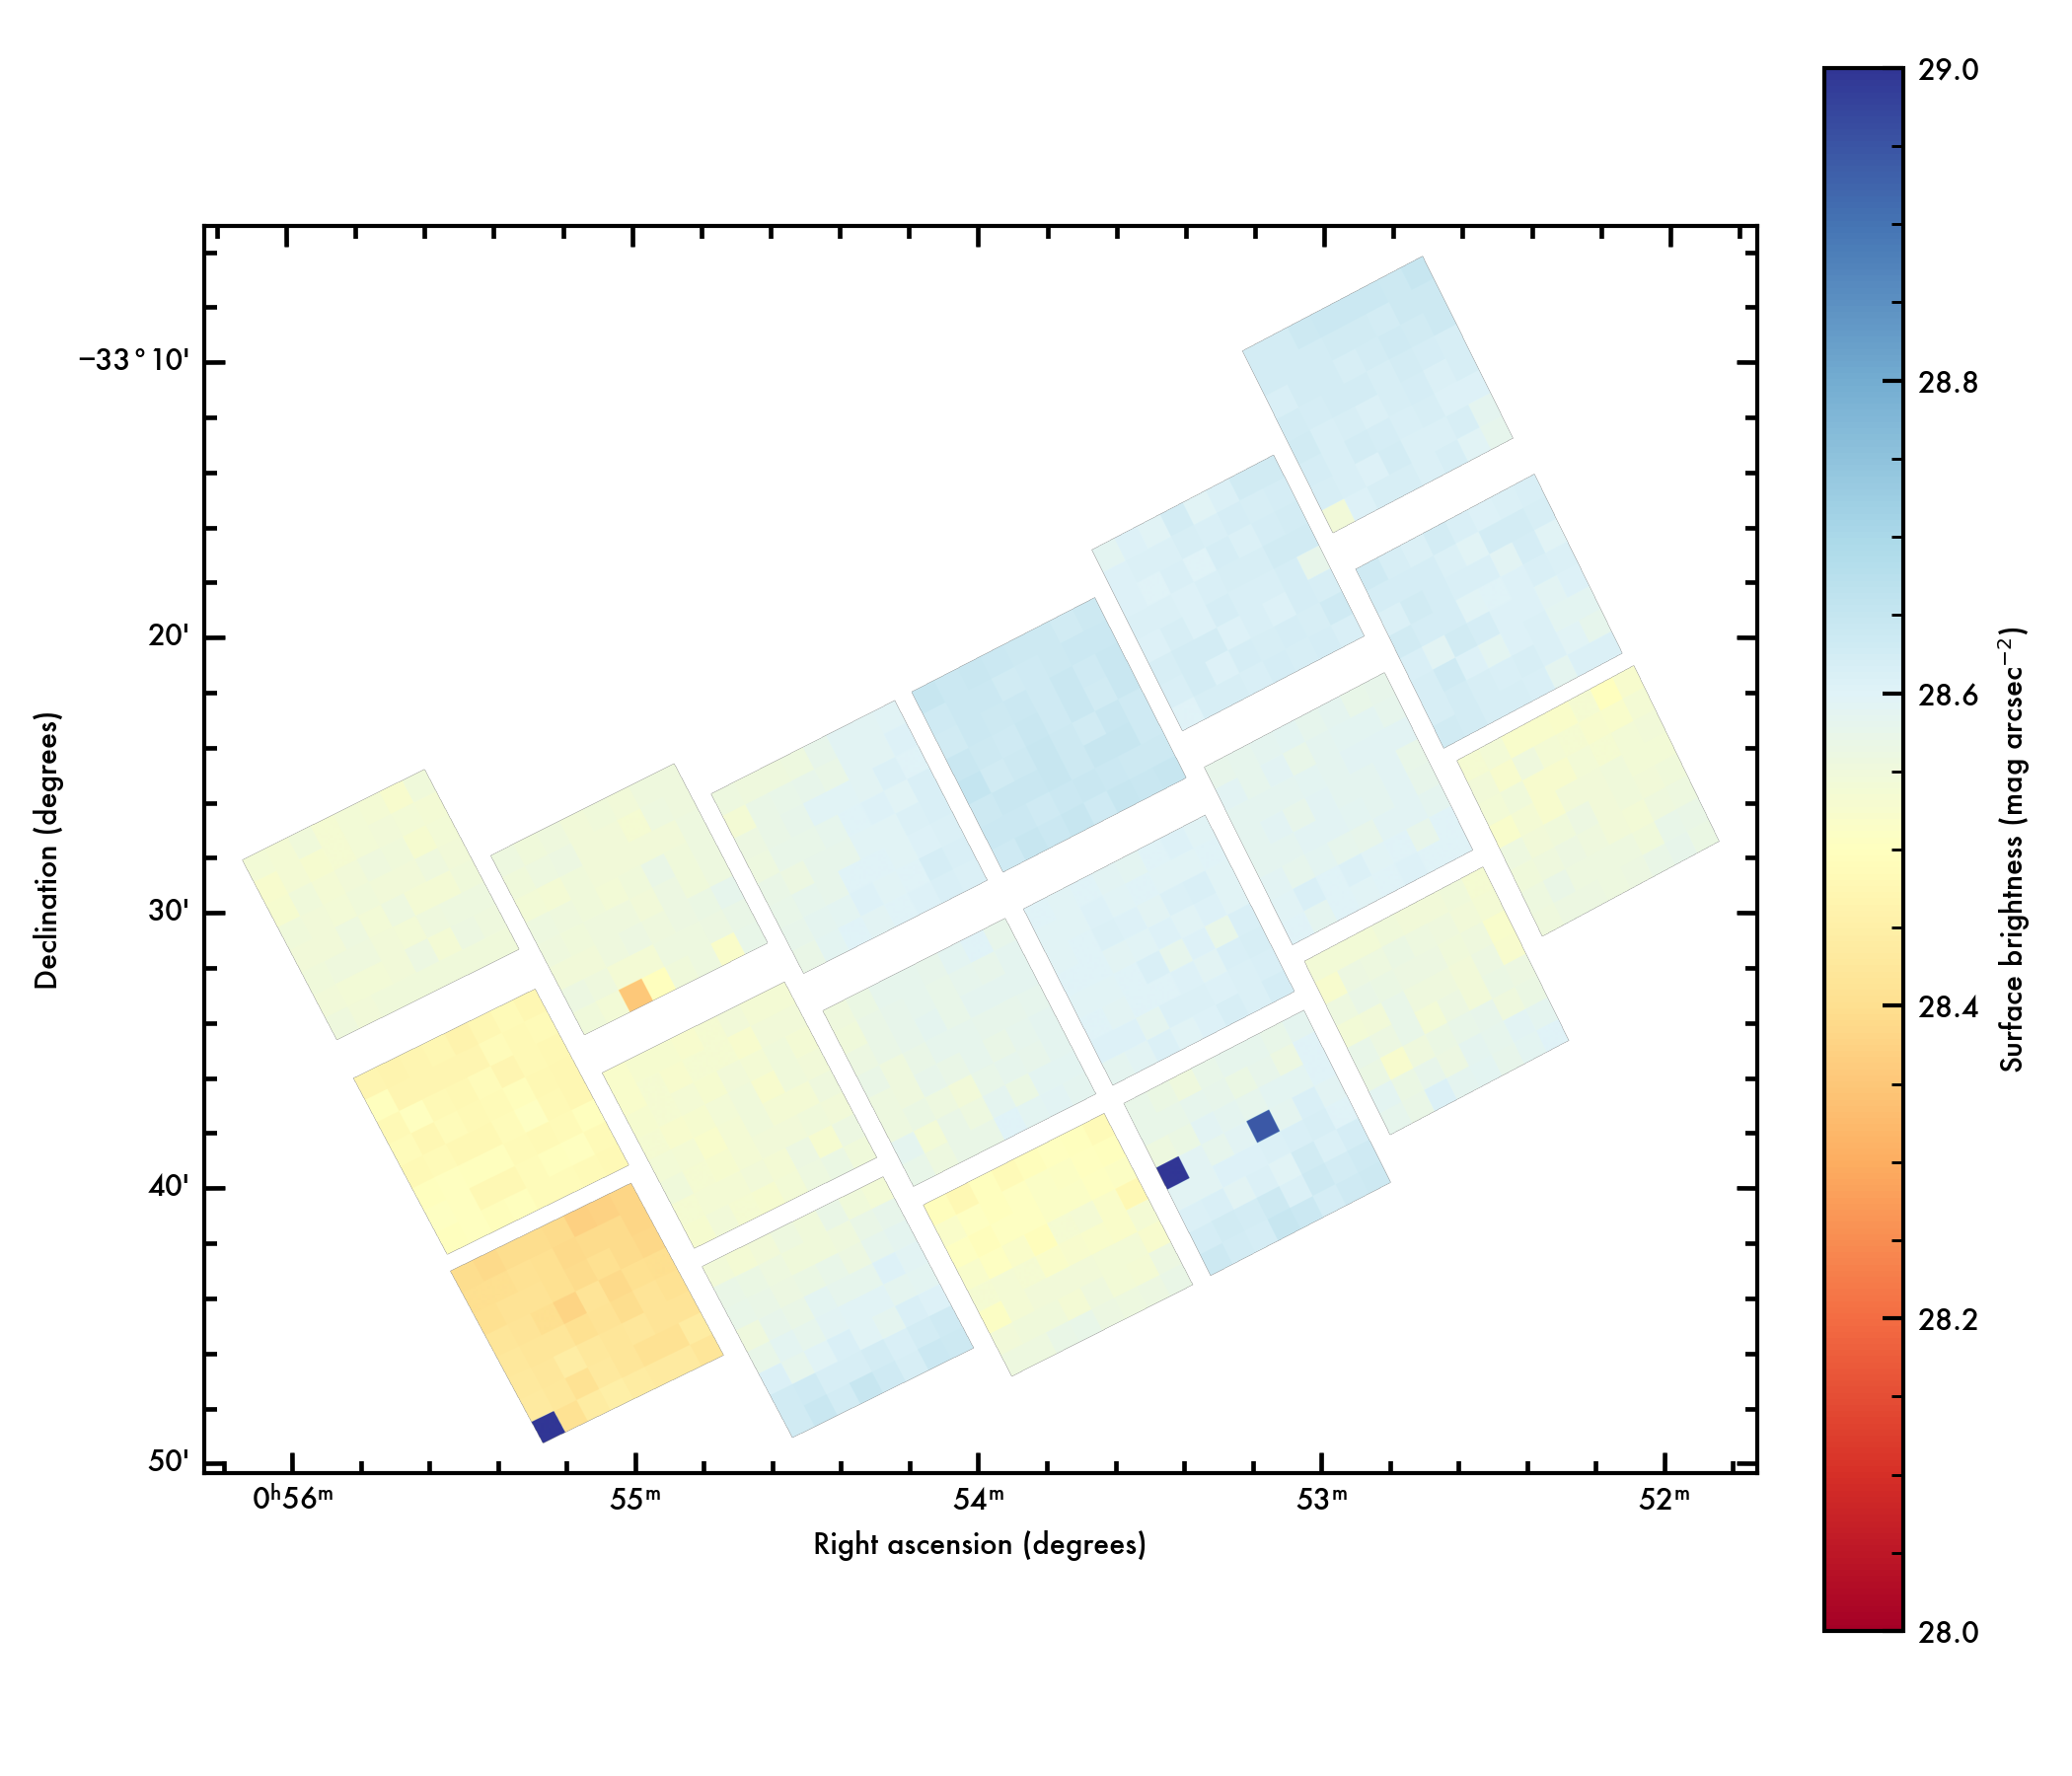
\includegraphics[trim={0 0 0 0}, clip, width=0.495\textwidth]{HWLAS77_WFI_F129_RA_013.502_DEC_-33.456_MJD_61577.00000_PA_027.09_stray_drz_scaled_fe2mu.png}
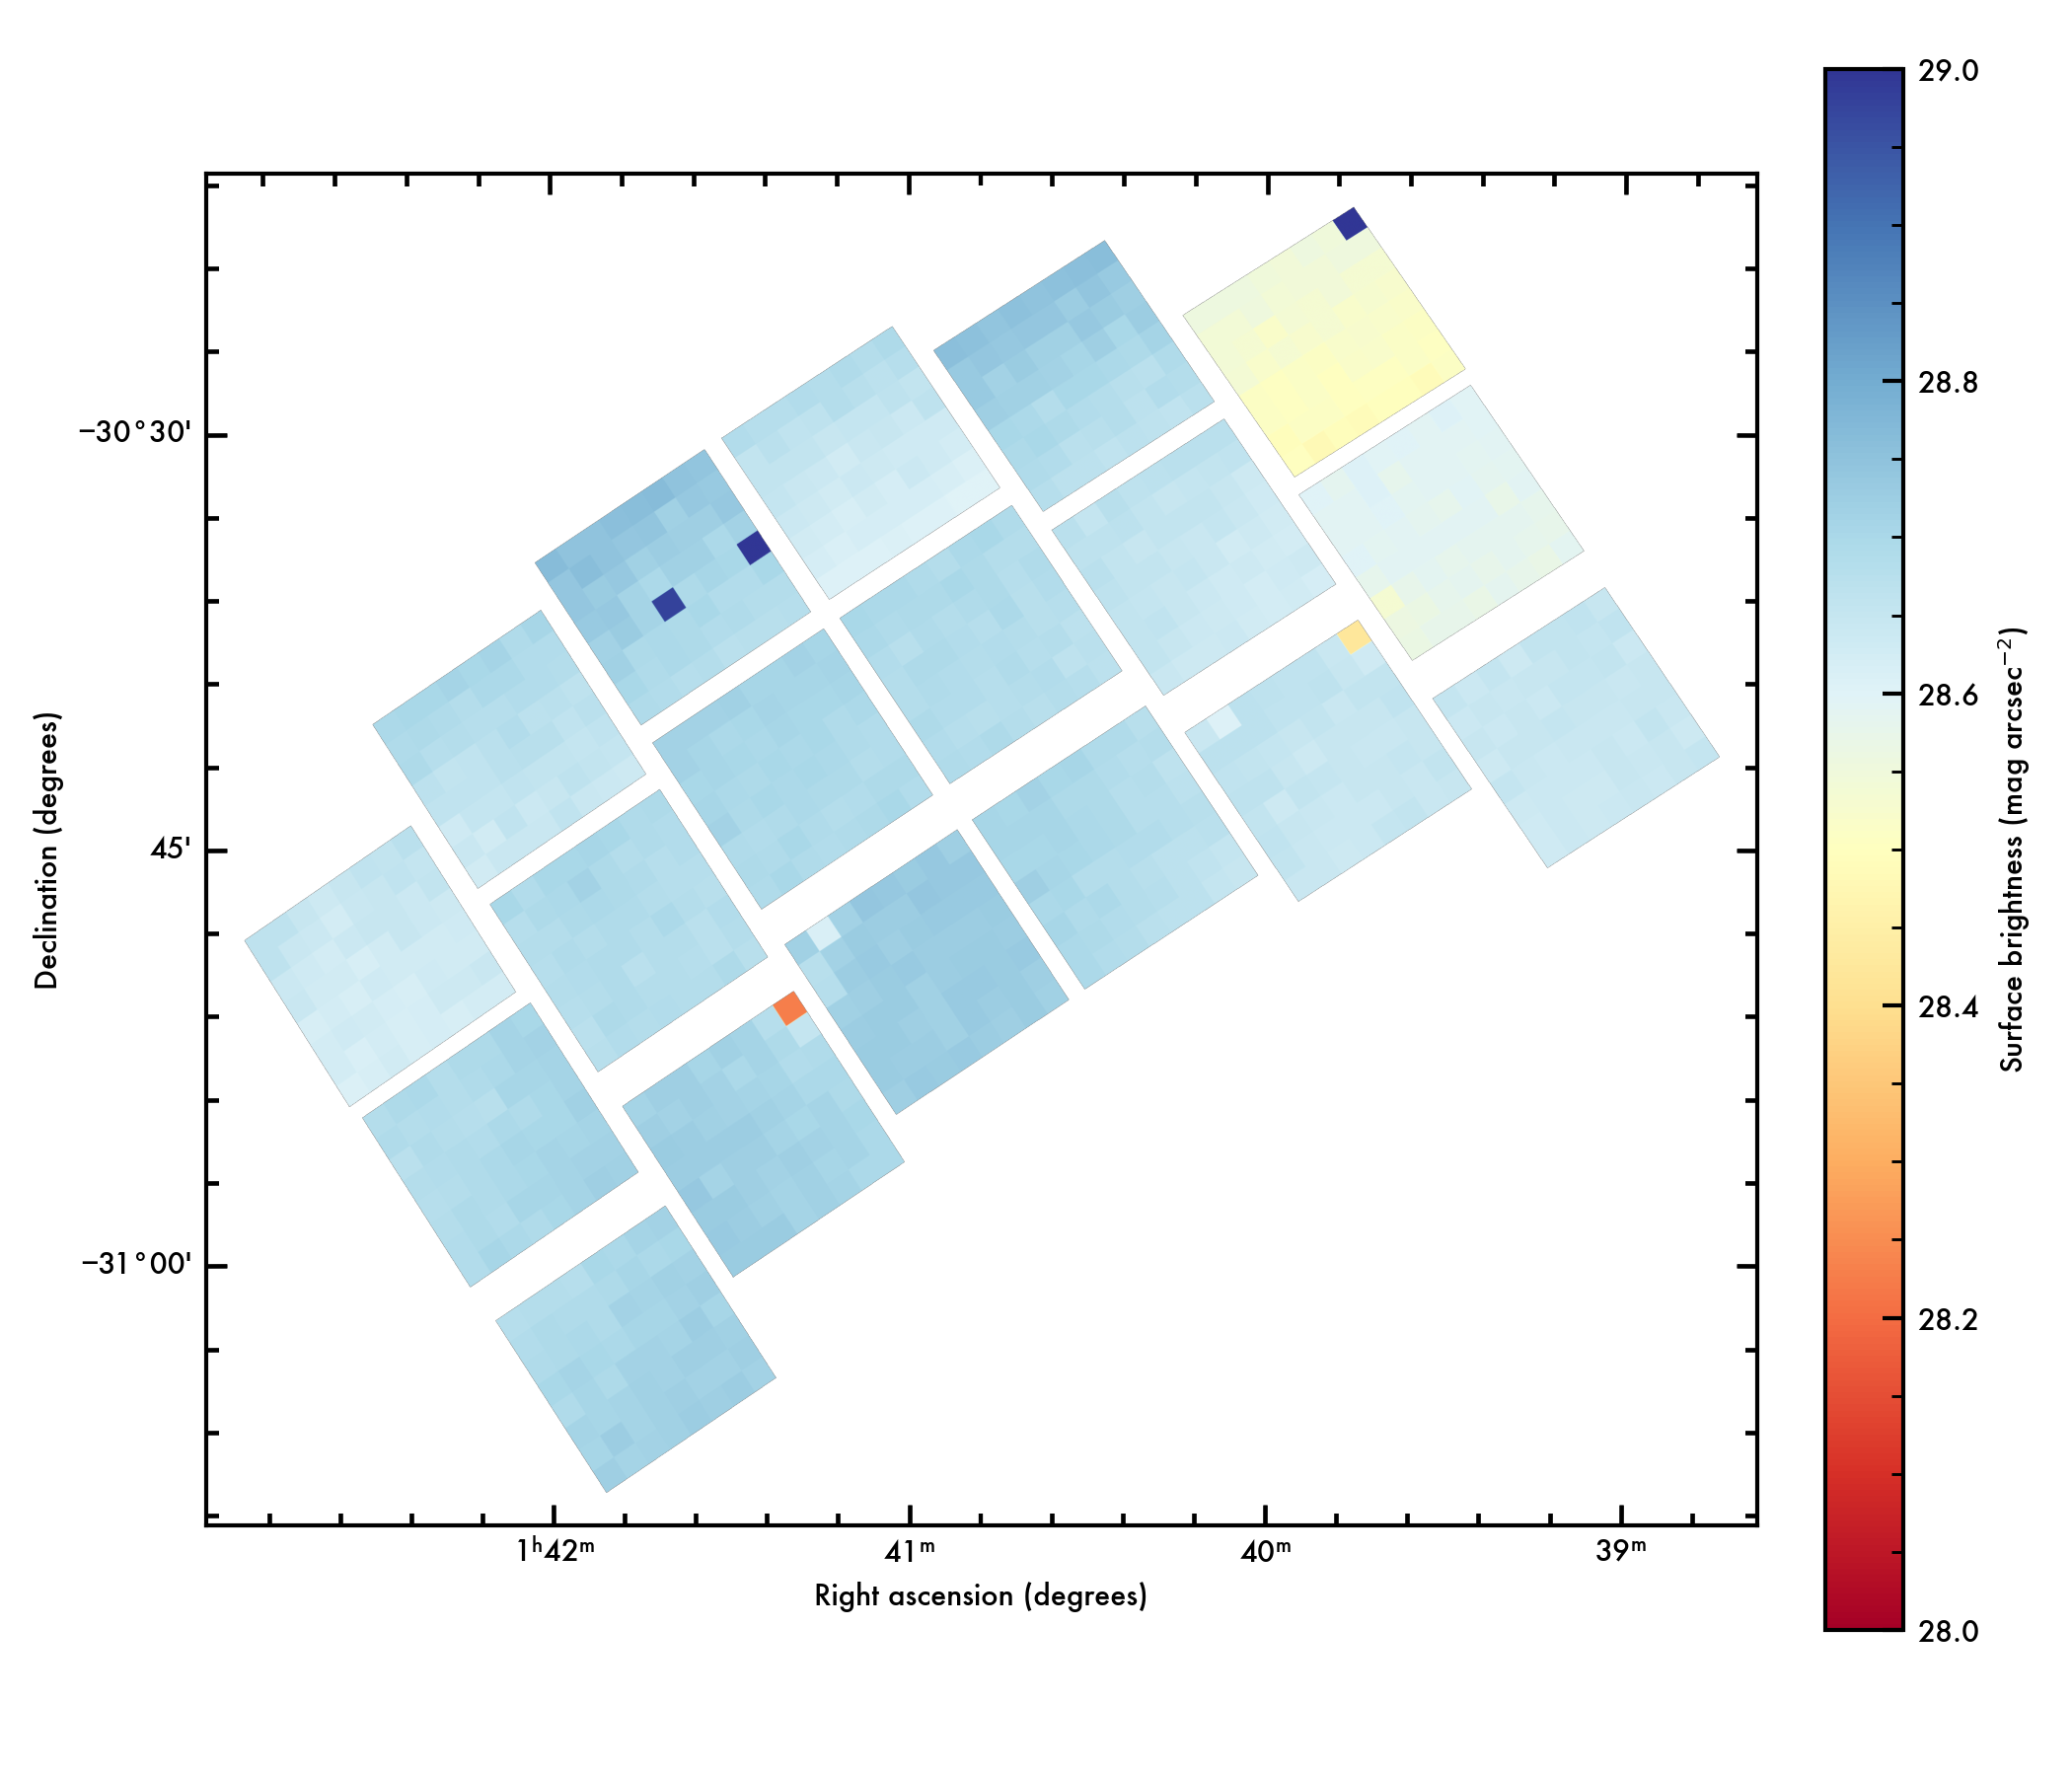
\includegraphics[trim={0 0 0 0}, clip, width=0.495\textwidth]{HWLAS77_WFI_F129_RA_025.194_DEC_-30.757_MJD_61577.00000_PA_-146.53_stray_drz_scaled_fe2mu.png}

\caption{Examples of stray-light background levels for the High Latitude Wide Area Survey as predicted by \texttt{ROSALIA}.} 
\label{fig:HWLAS_examples}
\end{center}
\end{figure*}


\section{The \texttt{ROSALIA} package} \label{sec:ROSALIA}

\texttt{ROSALIA} is available as a \texttt{Python} package\footnote{\texttt{pip install rosalia-wfi}: \url{https://pypi.org/project/rosalia-wfi/}} built to analyze the backgrounds on the Wide Field Instrument of Roman Space Telescope, combining detailed ray-tracing simulations with the all-sky photometric information from Gaia, 2MASS, WISE and JPL/Horizons. Available documentation \footnote{ReadTheDocs webpage: \url{https://rosalia.readthedocs.io/en/latest/}}describes the methodology to estimate the stray-light from out-of-field sources, as well as the interface to other packages like Galsim (PSF modeling of in-field stars), Zodipy \citep[Zodiacal light background estimations][]{2022A&A...666A.107S}. Contributions from the astronomical community can be submitted through its public repository \footnote{\texttt{Github ROSALIA:} \url{https://github.com/Borlaff/ROSALIA}}. The software is actively being upgraded with more tutorials and functionalities to support the Roman Cycle 1 and the commissioning activities.

\texttt{ROSALIA} is a Wide Field Science project funded through a NASA Grant (D.14 Roman 2022), as part of the ROSES/Nancy Grace Roman Space Telescope Research and Support Participation Opportunities.



\section{Summary}
\label{Sec:Summary}

The importance of low surface brightness studies has been highlighted by the 2020 Decadal Survey \citep{NAP26141}, emphasizing the need for effective data processing techniques beyond those of individual projects\footnote{2020 Decadal Survey, Section H.2.1 "Investment in Archives and Joint Analyses"}. The surface brightness limit of \emph{Roman}/WFI will depend on how well potential stray-light gradients are mitigated and/or avoided. The first analyses of \texttt{ROSALIA} under extreme conditions show that:

\begin{enumerate}
    \item Stray-light backgrounds can be produced by large scale features (\emph{Roman} Channel) or small scale structures (Dragon's Breath). 

    \item Small scale features can be efficiently suppressed by implementing small (20 arcsec) dithering shifts in the target.

    \item Large scale features produce dim patterns ($\mu_{\rm{S}}=27$ \magarc) even in the most extreme conditions (placing a 2 AB mag star on the Secondary leg region). The characteristic patterns produced when those regions are illuminated allows recognition and flagging on real images. 
\end{enumerate}

The expected stray-light levels on \emph{Roman}/WFI are extraordinarily dim $\mu = 25.0$ to 29.0 \magarc, showing an excellent efficiency of the Sun-shield and the optical blocking system. In the planning phase before \RST's launch, \texttt{ROSALIA} is serving as a figure-of-merit and advanced planning tool, allowing to optimize both calibration and science observations in the planning phase before launch, as well as providing valuable targets for Commissioning operations. \texttt{ROSALIA} will particularly benefit the High Latitude Imaging Survey (1700 deg$^2$), as it has one of the most stringent requirements on photometric uniformity for scales larger than the instrument FOV, and the Galactic Bulge Time Domain Survey, where small shifts can reduce the impact of Dragon's breath on the observations. Once during flight operations, \texttt{ROSALIA} will serve as an specialized calibration tool for the \RST\ observer community, enabling projects dedicated to the study of very extended ($>1$'), ultra-low surface brightness ($\mu\gtrsim29$ \magarc) structures in the Universe. 

\bibliographystyle{unsrtnat}
\bibliography{bibFile}{}


\end{document}